\section{The Photolyase Cryptochrome superfamily}\label{sec:PCSF}
Photolyases and cryptochrome are evolutionarily linked flavoproteins \parencite{conradPhotochemistryFlavoproteinLight2014}. Photolyases harvest light to repair DNA damage \parencite{sancarMechanismsDNARepair2016}. Cryptochromes were originally discovered to be blue light sensors regulating a vast array of functions \parencite{ahmadHY4GeneThaliana1993}, they are present both in plants and animals \parencite{meiEvolutionaryHistoryPhotolyase2015} and have since been discovered to serve a vast array of additional functions. Most, but not all cryptochromes are blue-light sensors. Cryptochromes and photolyases share a similar bilobial architecture made of a flavin adenine dinucleotide (FAD) binding C-terminal domain (pink Fig. \ref{fig:PCSF}) as well as an N-terminal Rossman folded domain (coloured lavender in Fig. \ref{fig:PCSF}, often referred to as \textalpha-\textbeta domain), able to bind an antenna chromophore. In some cryptochromes, the C-terminal domain is also capable of binding nucleotides \parencite{franzStructureBifunctionalCryptochrome2018}. In cryptochromes, these two domains (pink and lavender coloured Fig. \ref{fig:PCSF} (b)) combined are referred to as the photolyase homology region (PHr) In addition to those, cryptochromes feature an additional C-terminal extension (coloured orange in Fig. \ref{fig:PCSF} (b)) which can be of different lengths. The length of that domain is tightly linked to the various functions exhibited by cryptochromes \parencite{chavesFunctionalEvolutionPhotolyase2006}. In particular, the C-terminus of the \textit{Arabidopsis thaliana} cryptochrome is responsible for mediating the response to blue light \parencite{kongCterminalKinaseFragment2007}. 

\begin{figure}[H]
  \centering
  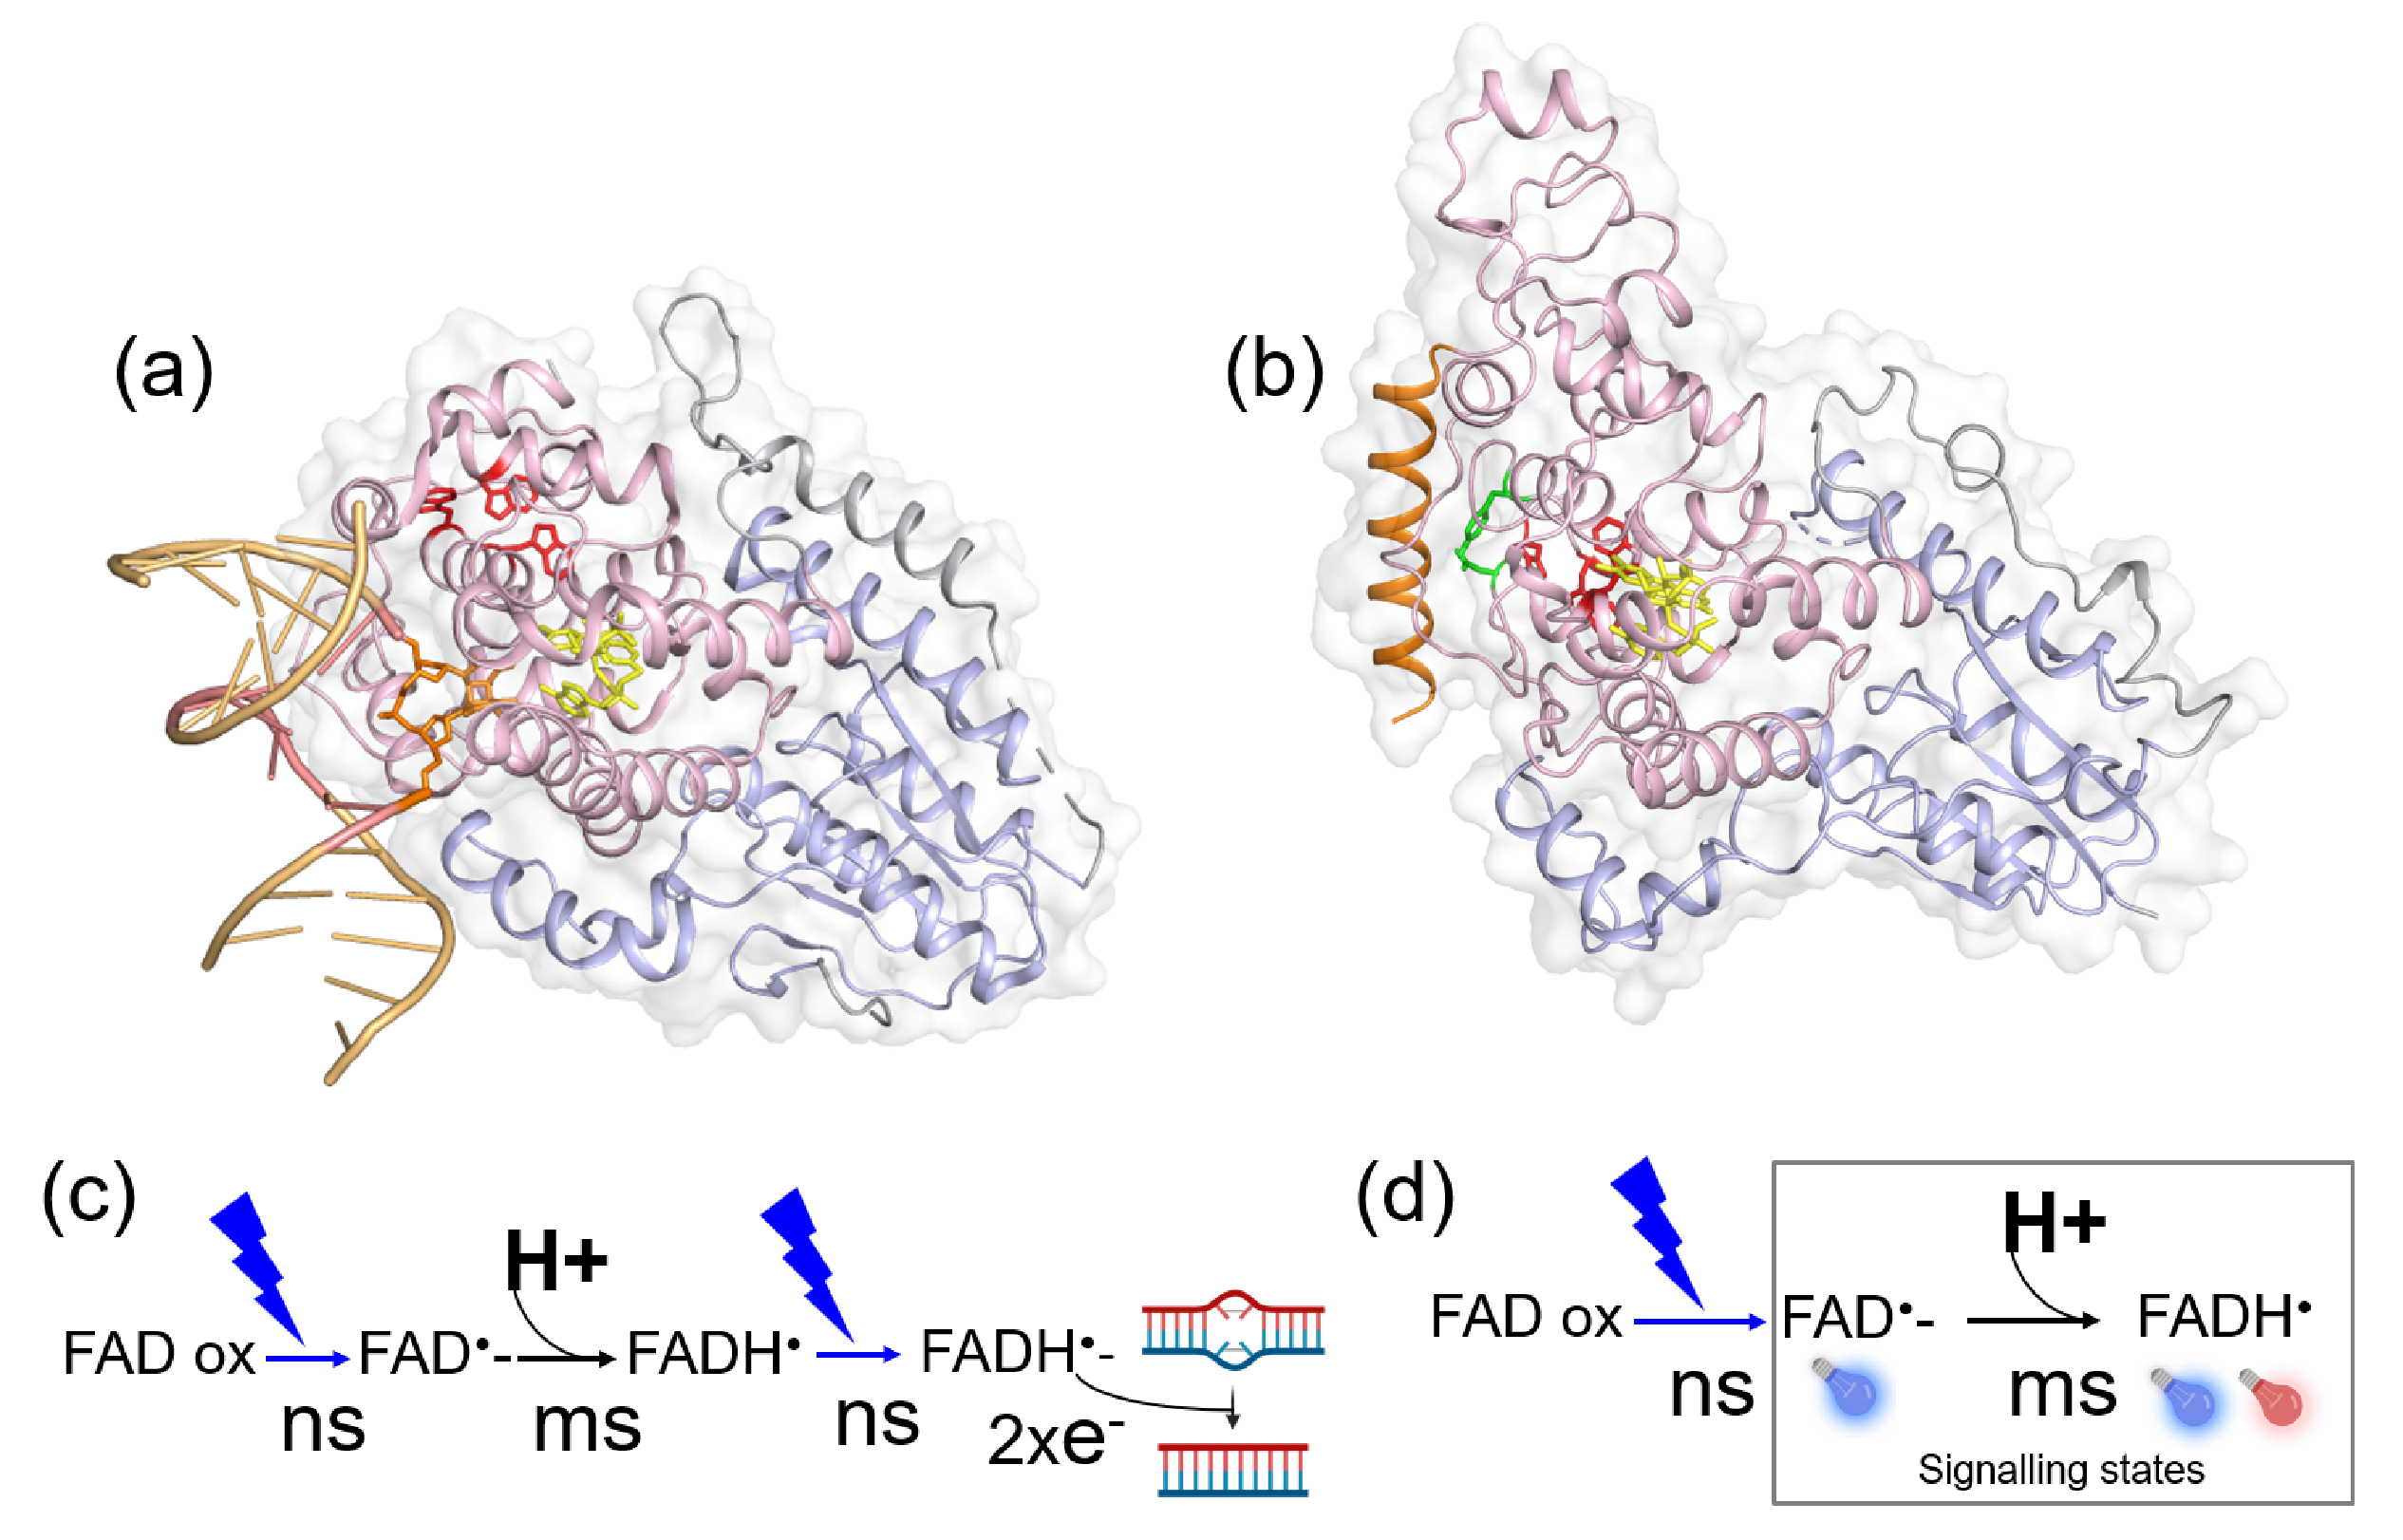
\includegraphics[width=\textwidth]{images/cracry/Photolyase_Cryptochromes.pdf}
  \hfill
  \caption{Overview of the Photolyase and Cryptochrome secondary structures and photoreactions. (a) Photolyase (Class II, CPD, \textit{Methanosarcina mazei}, pdb structure 7YEO) in complex with a DNA strand bearing a CPD type lesion. The N-terminal domain Rossman fold is coloured in lavender, the C-terminal domain is pink, the flavin cofactor is coloured yellow, and the DNA strand is orange. The electron transfer chain tryptophan triad is coloured red. (b) Cryptochrome (\textit{Chlamydomonas reinhardtii}, unpublished dark structure) N-terminal and C-terminal domains as well as the flavin cofactor and tryptophan triad are coloured identically as for (a). Additionally, the extra tyrosine forming the original tetrad of this cryptochrome is coloured green, as well as its proton donor. The C-terminal \textalpha-22 helix is coloured in orange. (c) Photoreaction of a photolyase: two subsequent photoreduction and protonation events are needed for DNA damage repair (d) Photoreaction of a cryptochrome with an oxidised ground state: A first photoreduction event happens, creating the semiquinone FAD containing signalling state, sensitive to blue light. This state can be further protonated to form a neutral semiquinone, sensitive to red light.}\label{fig:PCSF}
\end{figure}

In addition to their global architecture, Photolyases and Cryptochrome base their functions on the different redox states of their flavin cofactor. The ground state of all discovered photolyases is believed to be the oxidised state, the flavin cofactor must undergo two rounds of photoreduction by blue light to be catalytically active (Fig. \ref{fig:PCSF} (c), \cite{liuDynamicsMechanismsDNA2015}). Whether the flavin cofactor of cryptochromes is oxidised or semi-reduced (semiquinone) in their ground states is still up for debate \parencite{berndtNovelPhotoreactionMechanism2007, ozturkMechanismPhotosignalingDrosophila2014}. Although the recent discovery of a cryptochrome capable of signalling from both blue light and red light \parencite{beelFlavinBindingCryptochrome2012} suggests that both the oxidised flavin-containing and the semiquinone-containing cryptochromes could be physiological ground states, serving as photoreceptors for different wavelengths \parencite{kavakliPhotolyaseCryptochromeFamily2017}. In its ground state, the cryptochrome is photoreduced once, the change of polarity of the FAD sets in motion the signalling sequence of events. The signalling state can optionally be protonated, which extends its light sensitivity to red, and extends its lifetime \parencite{lacombatUltrafastOxidationTyrosine2019}.

The FAD is buried deep within the protein in both cryptochromes and FAD. Consequently, it cannot steal an electron from the solvent after excitation by a blue light photon. Instead, it takes it from a conserved tryptophan, and the electron-hole left by that transfer gets passed along an electron transfer chain formed by a conserved triad of tryptophans (red on Fig. \ref{fig:transferchain} \cite{liuDeterminingCompleteElectron2013, lacombatUltrafastOxidationTyrosine2019}). This triad (optionally completed by a fourth tryptophan \parencite{celliniStructuralBasisRadical2022} or tyrosine \parencite{franz-badurStructuralChangesBifunctional2019}, coloured green in Fig. \ref{fig:PCSF} (b)) carries the electron-hole until a solvent-exposed region, where it can be regenerated if an electron donor is present. after the first round of photoreduction, the semiquinone FAD is protonated by a nearby amino acid (teal on Fig. \ref{fig:transferchain} ) acting as a proton donor. 
\begin{figure}[H]
  \centering
  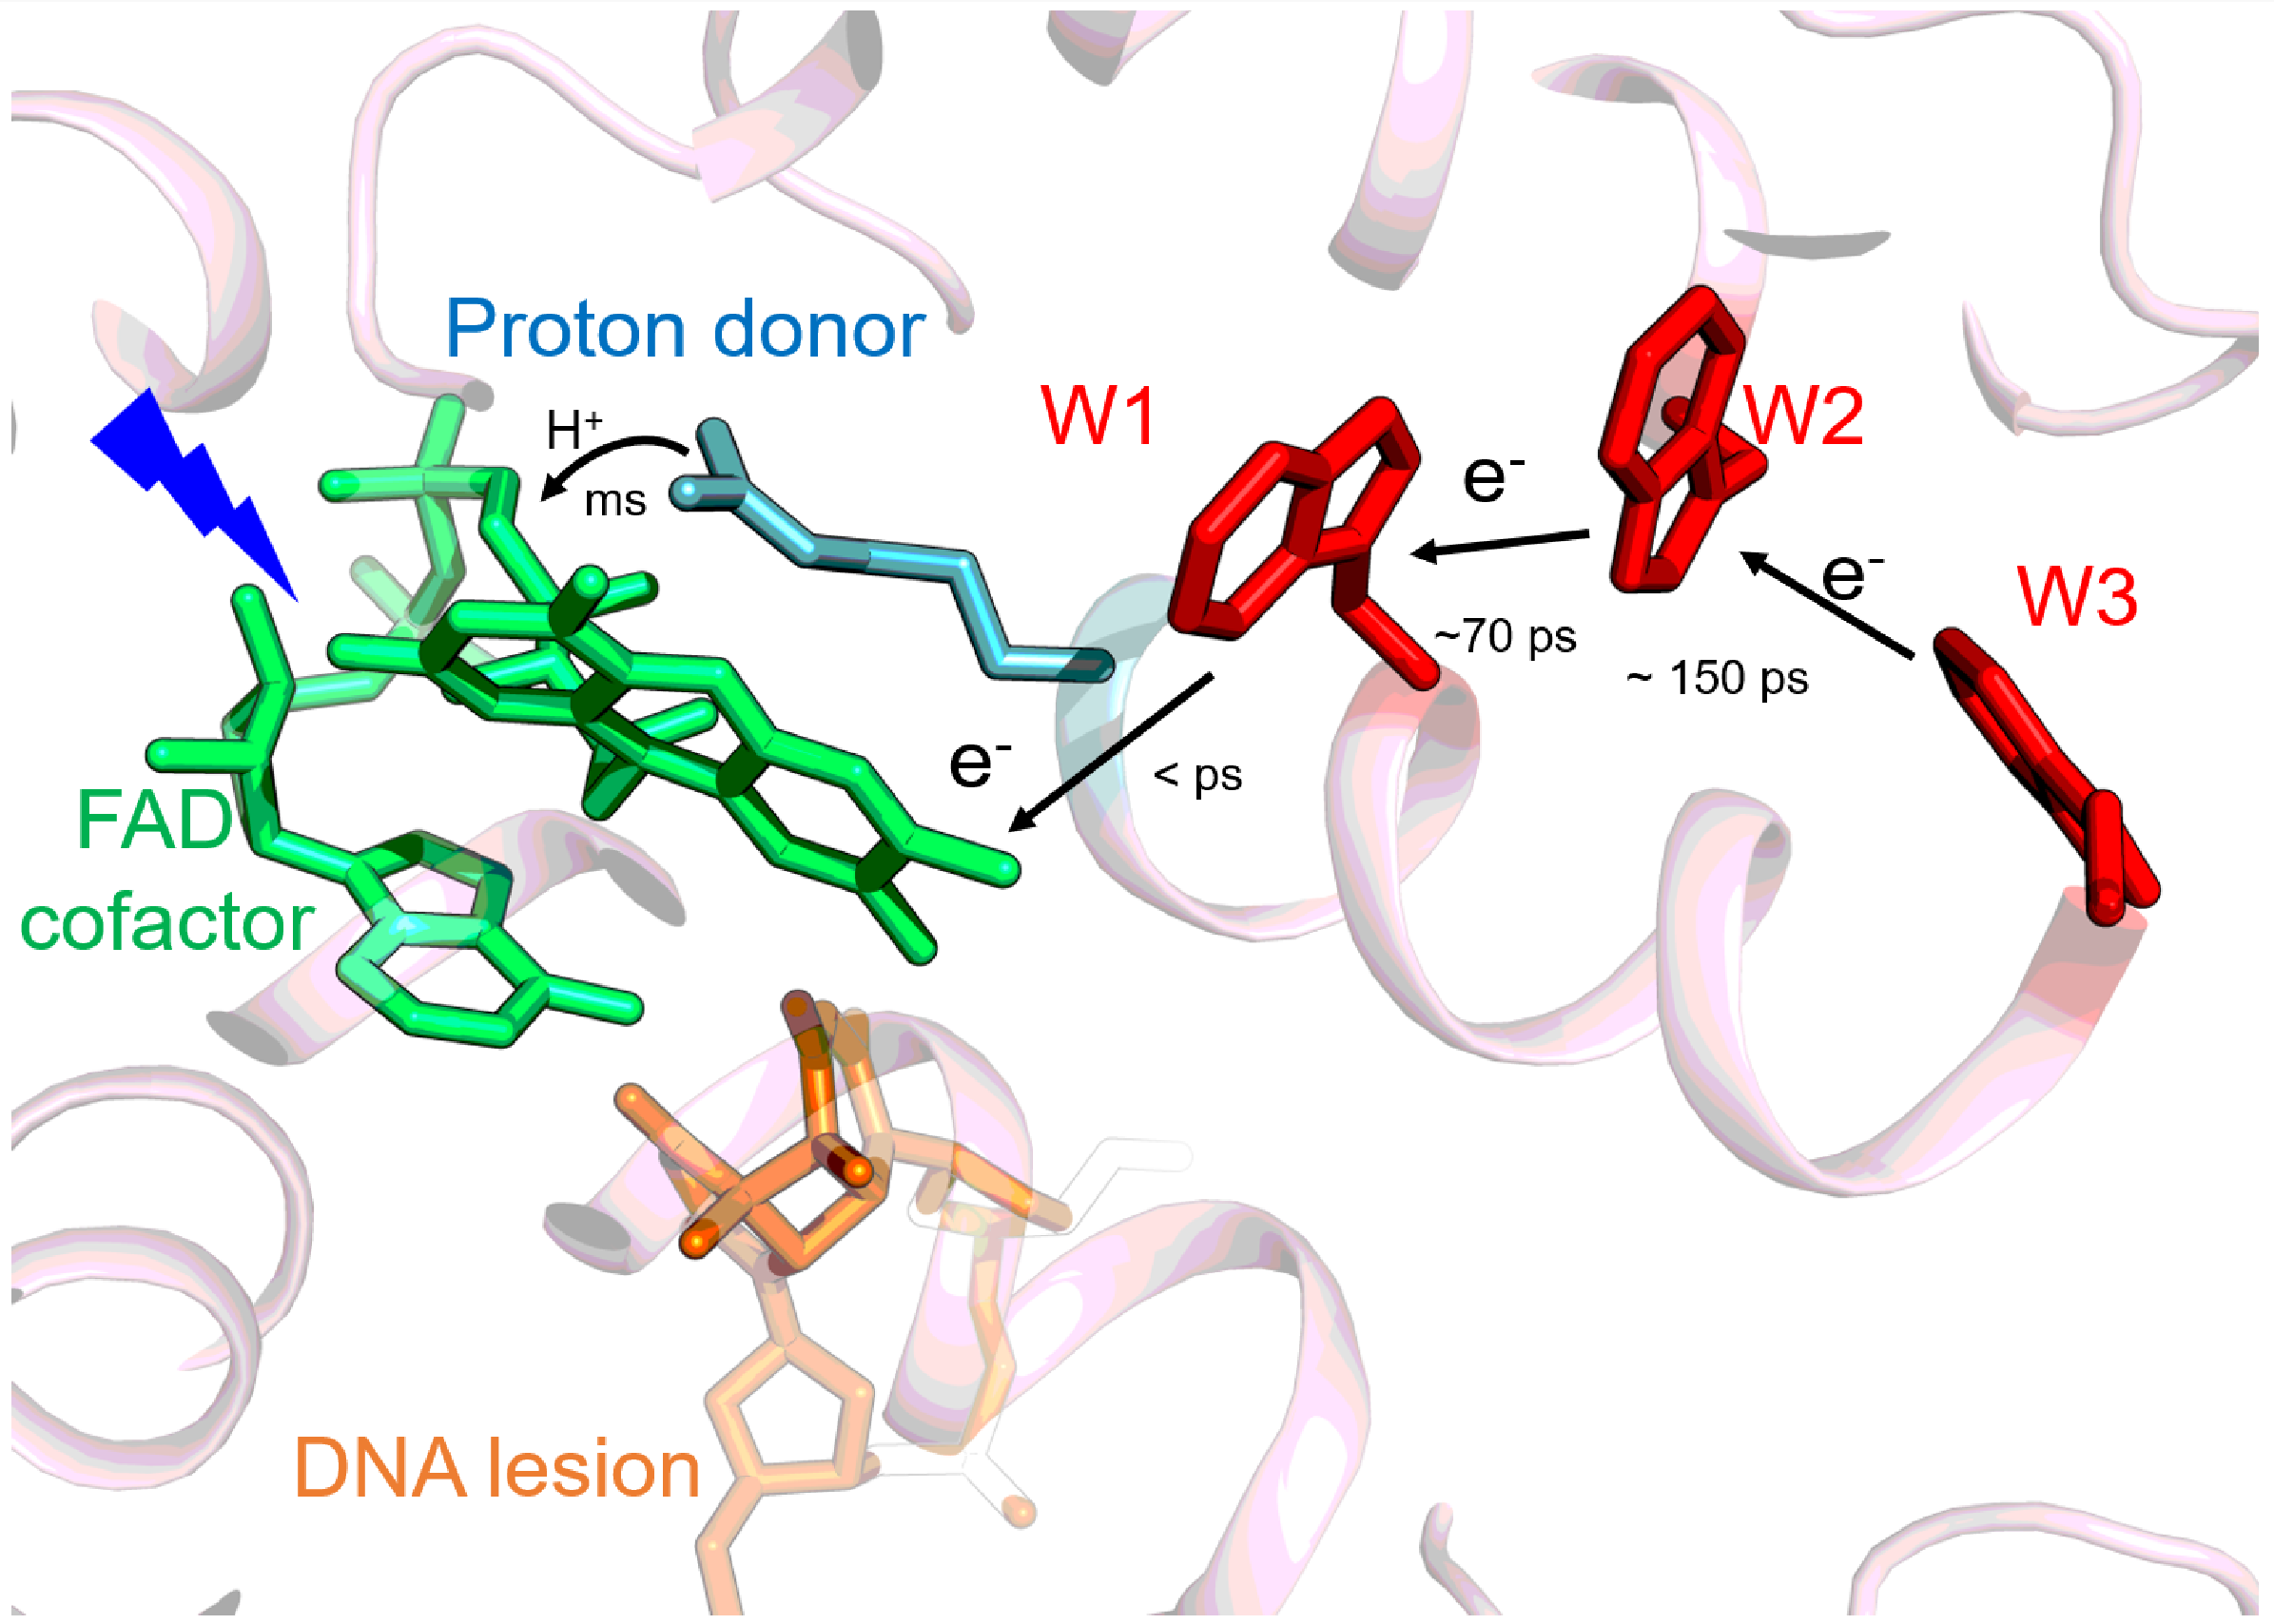
\includegraphics[width=\textwidth]{images/cracry/transfer_chain.pdf}
  \hfill
  \caption{Schematic representation of the Electron and proton transfer events underlying the photoreduction of cryptochromes and photolyases, using the structure of the Class II CPD photolyase of \textit{Methanosarcina mazei}. Less than a ps after it has absorbed a blue light photon, the FAD cofactor (green) steals an electron from a nearby tryptophan (red, W1). Several tens of ps later, W1 steals an electron from W2, and more than a hundred ps later, W2 steals an electron from W3 (all in red). W1, W2 and W3 are highly conserved in the photolyase and cryptochrome superfamily and form the electron chain triad. On the ms time scale, a nearby amino acid optionally gives a proton to the FAD (teal). }\label{fig:transferchain}
\end{figure}
Despite their drastically different functions, cryptochromes and photolyases share the same chassis, and framework of photoreduction scheme, followed by an electron transfer chain and a potential protonation. 

\subsection{Photolyases}

Exposure to UV damages the DNA in cells. UVB (315 - 280 nm) are most prone to creating DNA lesions \parencite{oakUVSkinPhotocarcinogenesis2018}. These lesions primarily occur in pyrimidine-rich segments of the cell's genome. The most abundant type of lesion present on a DNA strand after exposure to UV is Cyclobutane Pyrimidine Dimers (CPD) \parencite{oakUVSkinPhotocarcinogenesis2018}: two adjacent pyrimidine bases (thymine or cytosine) by their C5 and C6 atoms, forming a cyclobutane structure (Fig. \ref{fig:damagetype} (a)). Pyrimidine 6-4 pyrimidone photoproducts (6-4PP) are also created by exposure to UV: the two adjacent pyrimidine bases become linked covalently by their C4 and C6 atoms (Fig. \ref{fig:damagetype} (b)). These lesions bend the DNA strand and end up causing mutations down the line via replication errors. 

\begin{figure}[H]
  \centering
  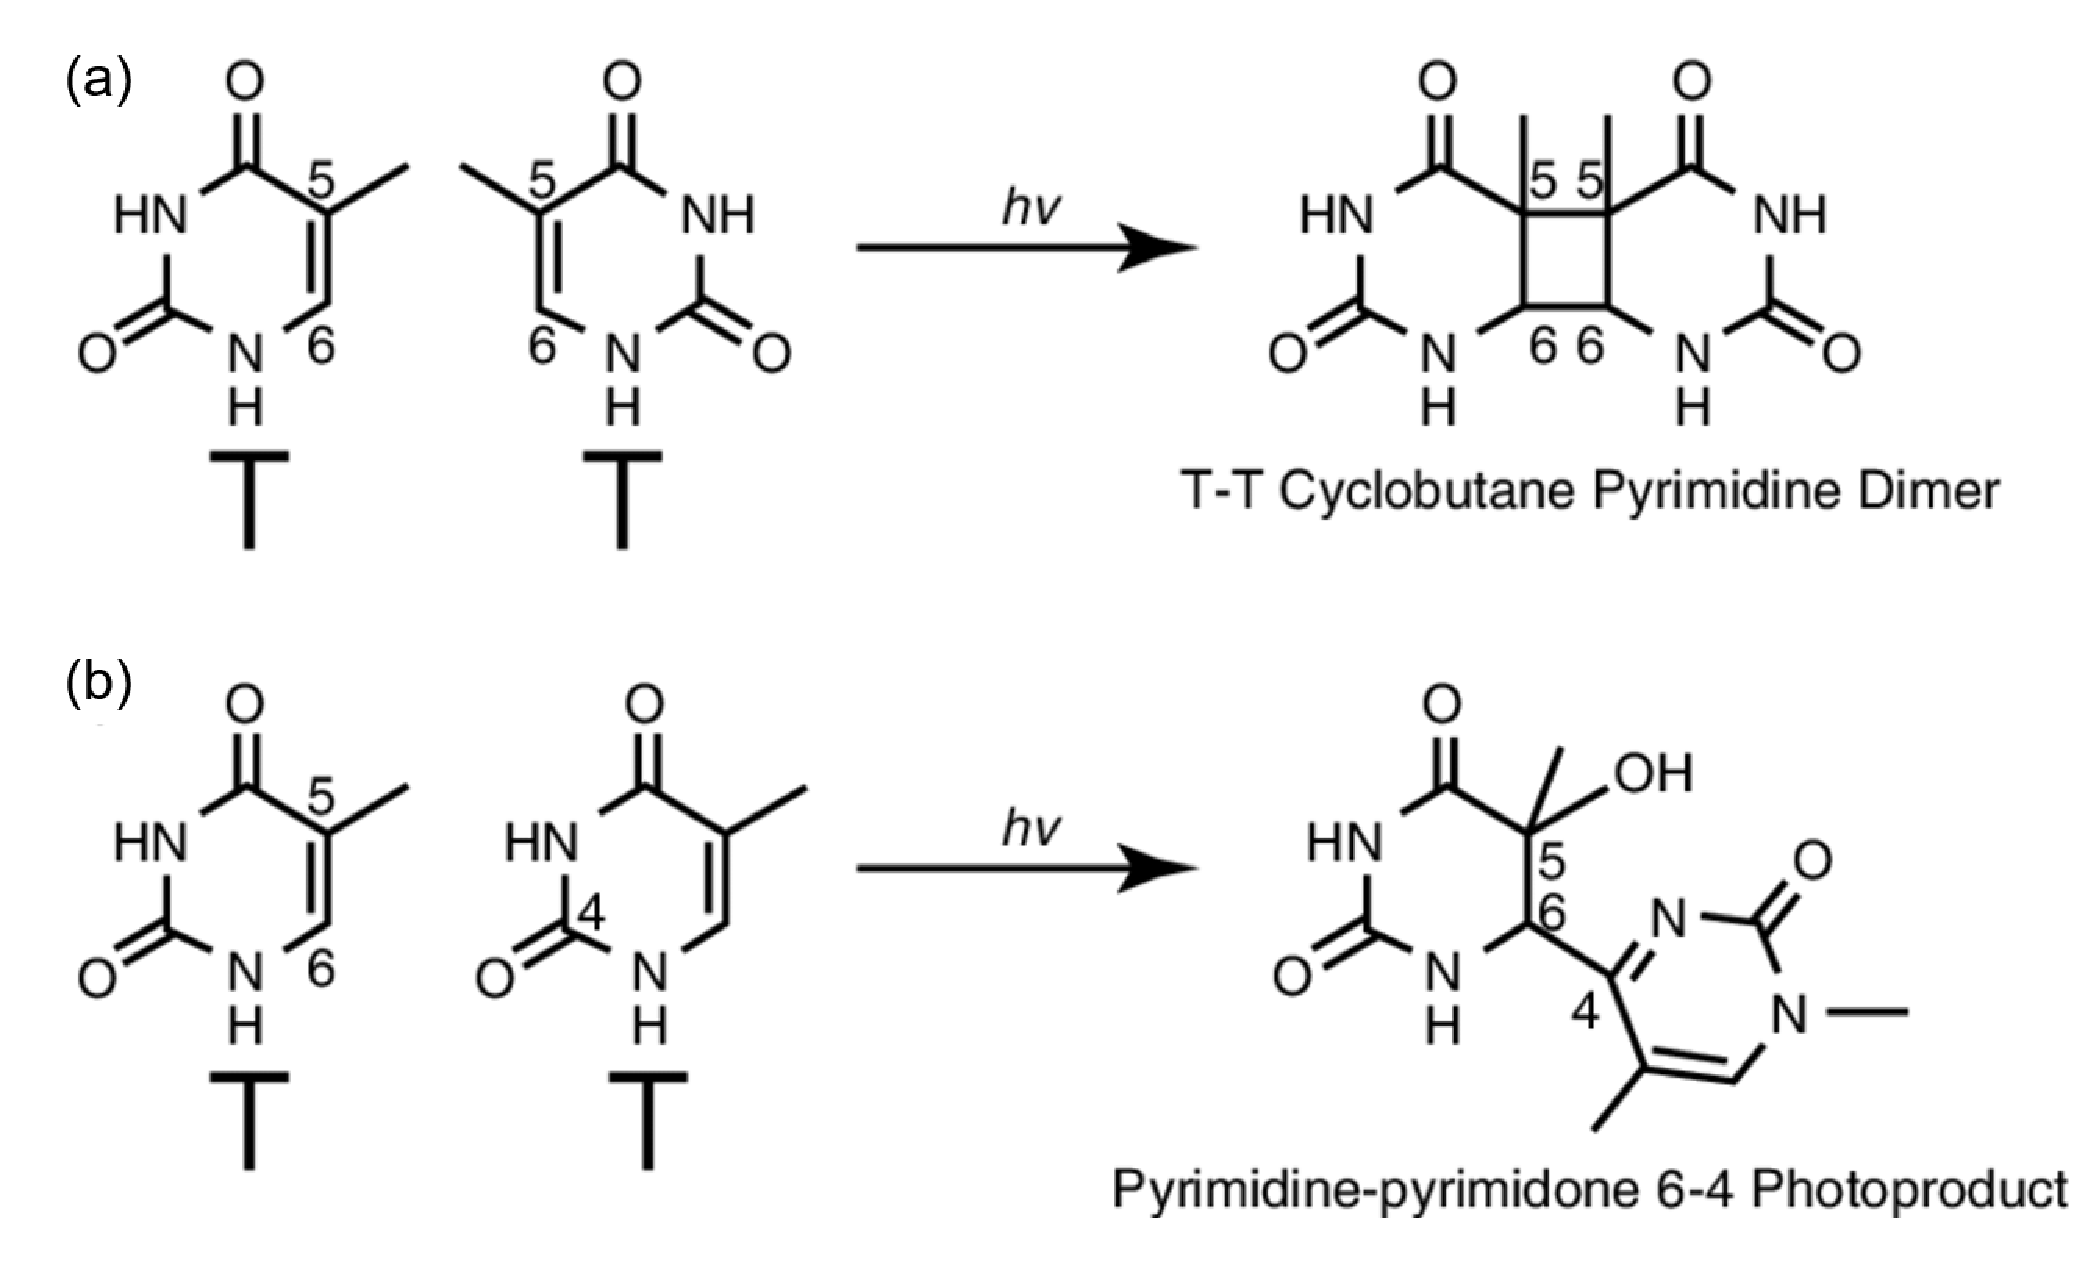
\includegraphics[width=\textwidth]{images/cracry/damagetypes.pdf}
  \hfill
  \caption{The main type of DNA lesion occurring on a DNA strand after exposure to UV. (a) Upon UV exposure, two following pyrimidine bases (here, thymine) become covalently bonded twice, by their respective C6 and C5 atoms, forming a cyclobutane pyrimidine dimer (b) Upon UV exposure, a covalent bond forms between the C6 atom of the first base and the C4 atom of the second base, forming a dimer called a 6-4 photoproduct. Reproduced from \parencite{oakUVSkinPhotocarcinogenesis2018}}\label{fig:damagetype}
\end{figure}
In humans, the mutations caused by these DNA lesions go on to be the leading cause of skin cancer \parencite{cadetUltravioletRadiationmediatedDamage2005}. Of note, humans use a complex enzymatic pathway, called nucleotide excision repair (NER) to repair DNA lesions. Most organisms use a more straightforward approach: a single protein powered by light, the photolyase, identifies and repairs the lesion. Photolyases are one of the three discovered photoenzymes, the only enzymes known to physiologically harvest light to catalyse chemical reactions \parencite{bjornPhotoenzymesRelatedTopics2018}. 

The existence of a light-powered DNA repair enzyme was first discovered in 1958 by Claud S. Rupert, when he realised that virus DNA which had been inactivated by exposure to UV radiation could be reactivated in the presence of a cell lysate of E. coli, and under visible light exposure \parencite{rupertPHOTOREACTIVATIONVITROULTRAVIOLET1958}. The enzyme responsible for this function was only later identified some 25 years later \parencite{sancarDNAPhotolyasesPhysical1990}. The first photolyase whose structure was solved with X-ray crystallography was the CPD photolyase of \textit{Escherichia coli} \parencite{parkCrystalStructureDNA1995}. The structure of a photolyase from \textit{Drosophila melanogaster}, capable of repairing 6-4PP was later solved \parencite{maulCrystalStructureMechanism2008}.

It was later determined that there were several families of CPD photolyases \parencite{meiEvolutionaryHistoryPhotolyase2015}. The \textit{E. coli} CPD photolyase previously mentioned belongs to the Class I subfamily, prevalent among prokaryotes. In Eukaryotes, the Class II CPD photolyase family is more present. The first structure of a Class II photolyase solved was that of \textit{Methanosarcina mazei} \parencite{kiontkeCrystalStructuresArchaeal2011}, revealing a more compact fold. A third subclass of photolyases was more recently identified \parencite{ozturkPurificationCharacterizationType2008}.

It is nowadays accepted that the common ancestor to the photolyase-cryptochrome superfamily was likely a Class I CPD photolyase \parencite{mullerStructuralBiologyDNA2009}. 

\subsection{Cryptochromes}\label{sec:cryptochrome_families}
Cryptochromes owe their cryptic name to the vast array of functions that they perform, their ubiquitous nature and the lack of knowledge of their mechanism. In 1993, a gene was identified as responsible for the elongation of the hypocotyl as a response to blue light in \textit{Arabidopsis thaliana} \parencite{ahmadHY4GeneThaliana1993}. It was later discovered that this gene encoded the first ever discovered blue-light sensor of plants, the cryptochrome. Cryptochromes were also identified in other plants, as responsible for flowering, as well as a variety of other functions\parencite{kavakliPhotolyaseCryptochromeFamily2017}. This already vast set of functions was extended by the discovery of cryptochromes in \textit{Drosophila melanogaster}, as photoreceptors regulating the circadian clock \parencite{emeryCRYDrosophilaClock1998,stanewskyCrybMutationIdentifies1998}. Mammals also feature cryptochromes, involved in the circadian clock \parencite{vitaternaDifferentialRegulationMammalian1999}. 

Animal cryptochromes (such as that of \textit{Drosophila melanogaster} share a strong homology with 6-4 photolyases, while plant cryptochromes are closer to Class I CPD photolyases \parencite{kavakliPhotolyaseCryptochromeFamily2017}. As a consequence, cryptochrome feature C-terminal domains (coloured orange on Fig. \ref{fig:PCSF} (b)) of extremely variable length (3 to 300 amino-acid long), which appear to be tightly linked to their function \parencite{partchRoleStructuralPlasticity2005}. This strong variability allows different cryptochromes to interact with different partner proteins, partially explaining how they can regulate seemingly unrelated functions \parencite{meiEvolutionaryHistoryPhotolyase2015}. A family of cryptochromes deprived of C-terminal (CRY-DASH, for \textit{Drosophila}, \textit{Arabidopsis}, \textit{Synechocystis}, and \textit{Homo}) domain was also identified \parencite{brudlerIdentificationNewCryptochrome2003}. Members of this family originate from a CPD photolyase, as is the case for plant cryptochromes, despite CRY-DASH being also present in animals \parencite{chavesCryptochromesBlueLight2011}. CRY-DASH cryptochromes have retained their ability to repair CPD DNA lesions, but only on single-strand DNA, and no longer on double-stranded DNA \parencite{selbyCryptochromePhotolyaseClass2006}. 

Many organisms possess several cryptochromes, as is the case for \textit{Arabidopsis thaliana} which possesses two plant-like cryptochromes (CRY1 and CRY2), and a CRY-DASH (CRY3) \parencite{kavakliPhotolyaseCryptochromeFamily2017}. Accordingly, a unique type of animal-like cryptochrome (animal-like cryptochrome) was more recently discovered in \textit{Chlamydomonas reinhardtii}, despite \textit{Chlamydomonas reinhardtii} already having a plant-like cryptochrome and two CRY-DASH \parencite{beelFlavinBindingCryptochrome2012}. CraCRY is sensitive to both blue and red light and has retained its 6-4PP repair function \parencite{franzStructureBifunctionalCryptochrome2018}. 

\chapter{The mechanism of DNA repair by the Class II CPD photolyase of \textit{Methanosarcina mazei}}\label{chap:MmCPDII}

\vspace{10mm}

\section{Studying photolyases with XFEL radiation}

Despite their fame as the first characterised photoenzyme and the number of crystal structures already determined \parencite{mullerStructuralBiologyDNA2009}, the mechanism of DNA repair by photolyases had not - until very recently \parencite{maestre-reynaVisualizingDNARepair2023a, christouTimeresolvedCrystallographyCaptures2023a}, been investigated with TR-MX. This is perhaps partially explained by their extreme sensibility to specific radiation damage in the form of photoreduction of the flavin by the X-ray beam \parencite{kortDNAApophotolyaseAnacystis2004}, which can go as far as eliciting DNA repair \parencite{meesCrystalStructurePhotolyase2004}.  This is why the study of DNA repair by photolyases is only achievable using the TR-SFX technique at an XFEL, where damage-free structures can be obtained. 

\section{Visualizing the DNA Repair Process by a Photolyase at Atomic Resolution.}\label{sec:prior_MmCPDII}
Only the scope, context and results of our DNA repair paper are summarised here.

The first step of the DNA repair mechanisms is photoreduction (Fig. \ref{fig:PCSF} (c)). Photoreduction of the Class II photolyase of \textit{Methanosarcina mazei} (\textit{Mm}CPDII) has been investigated by the collaboration network previously mentioned, before the beginning of this PhD \parencite{maestre-reynaSerialCrystallographyCaptures2022}, bringing the FAD cofactor of the photolyase to the fully reduced  FADH\textsuperscript{-} state. Once the photoreduction is over, DNA repair is possible upon an additional excitation, transiently bringing the FAD to the FADH\textsuperscript{•-}, which causes an electron to be transfered to the CPD. 

Based on extensive ultrafast spectroscopy studies \parencite{zhangPhotolyaseDynamicsElectrontransfer2017}, a mechanism for the repair of CPD has been proposed: First, a forward electron transfer from the reduced cofactor FADH\textsuperscript{-} produces the CPD radical anion (T<>T)\textsuperscript{•-}, where the excess electron may be shared between the two pyrimidines. The \(C5-C5'\) of the CPD is then cleaved first, producing (T\_T)\textsuperscript{•-}. after that is the \(C6-C6'\) bond cleaved too (this step is visible in visible on Fig. \ref{fig:DNArepair_schem} (b)), yielding (T+T)\textsuperscript{•-}. Finally, there is a transfer of one electron from the anionic radical thymine, back to the FAD cofactor, regenerating the FADH\textsuperscript{-} state and neutral thymine. One of the goals of this study was to catch these spectroscopic reaction intermediates to understand how the active site of the photolyase stabilises them. 

These intermediates were investigated via a time series from 100 ps to 10 ns time-domain (100, 250, 450, 650 ps; 1, 2, 3.35, 6, 10 ns), collected with a pump-probe scheme using the pulse of a fs laser as the pump on beamline ALVRA at SwissFEL.

Even bearing a CPD lesion, a double strand of DNA retains an interaction between adenosines and thymines pairs of opposing strands in the damaged region: the CPD lesion is still within the double stranded helix \parencite{parkCrystalStructureDNA2002} It is only when the strand is paired with a CPD photolyase that the CPD region flips out of double-stranded conformation to lodge within a specific groove (visible in Fig. \ref{fig:DNArepair_schem} (a), \cite{maestre-reynaTwistTurnRevised2018}). The mechanism underlying the transition from that regionally single-stranded repaired set of based to an annealed and freed-out double strand of DNA is unknown (the isomorphous \(F_{obs}(repaired\ bases) - F_{obs}(dark)\) map for lesion repair is represented over the ground state model in Fig. \ref{fig:DNArepair_schem} (b)). This is especially interesting as the photolyase has a much lower affinity for repaired DNA, indicating that it can recognise the lesion specifically, and kicks it out once the repair is over. That last step is visible in Fig. \ref{fig:DNArepair_schem} (c).

This unknown conformational mechanism was investigated by a second pump-probe time series spanning from 10 ns to 200 \textmu s (10, 100, 500 ns; 25, 200 \textmu s), collected at SACLA where the pump was the pulse of a ns laser.

\begin{figure}[H]
  \centering
  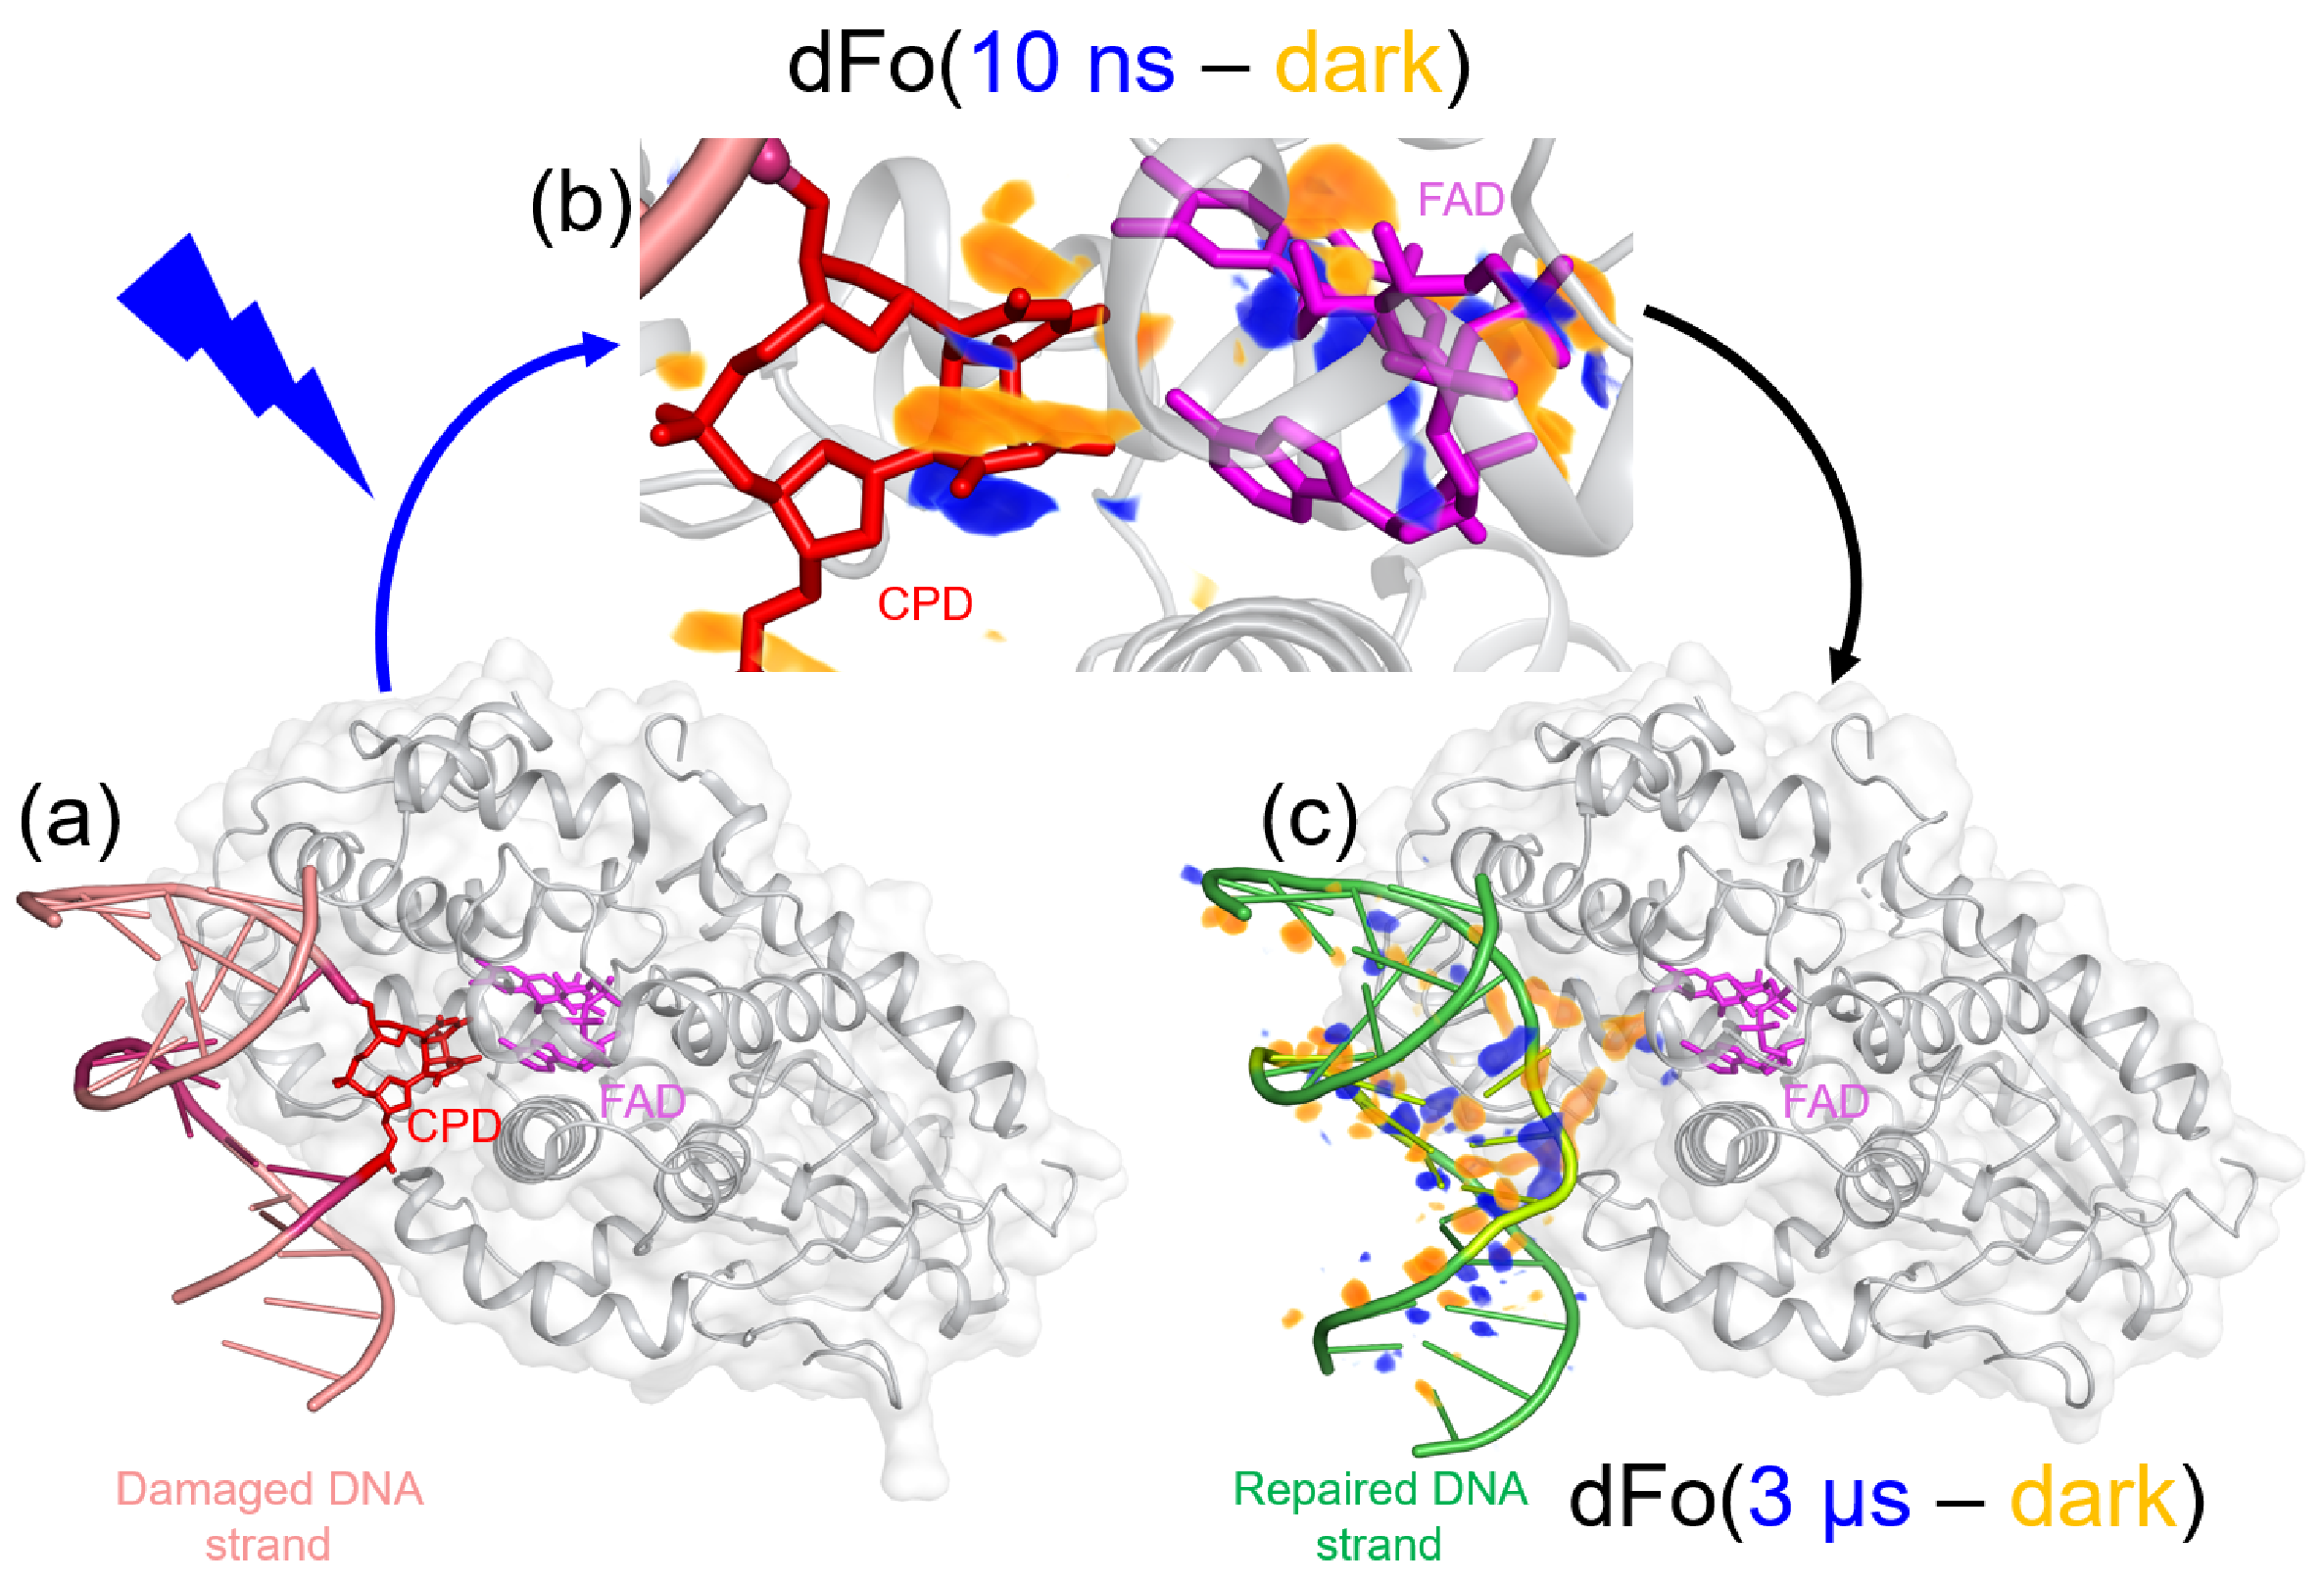
\includegraphics[width=\textwidth]{images/cracry/Science2023.pdf}
  \hfill
  \caption{Schematic representation of the reaction visualised via TR-SFX in \cite{maestre-reynaVisualizingDNARepair2023a}. (a) Dark \textit{Mm}CPDII structure with a fully reduced FADH- (magenta) in complex with a damaged DNA strand (rose) bearing a CPD (red). (b) Close-up view of the CPD pocket with overlaid \(F_{obs}(10 ns) - F_{obs}(dark)\) electron difference map (contoured at 3.5 \textsigma level, negative peaks in gold and positive peaks in blue). Colour codes same as before (c) Structure of \textit{Mm}CPDII with a repaired, annealed DNA double strand (green) exiting the protein complex, as evidenced by the overlaid \(F_{obs}(200 \mu s) - F_{obs}(dark)\) electron difference map (contoured at 3.5 \textsigma level, same colour scheme).}\label{fig:DNArepair_schem}
\end{figure}

The DNA repair mechanism can only be initiated when the FAD cofactor of the photolyase is fully reduced (FADH-). Therefore, the experiment required that crystals of fully reduced \textit{Mm}CPDII in complex with damaged DNA could be produced and maintained in a reducing (anaerobic) atmosphere, away from blue light, long enough to be brought in front of the beam. 

To meet that standard, \textit{Mm}CPDII crystals were grown no more than 12 hours before being shot with the X-ray beam. \textit{Mm}CPDII samples, frozen with 20 \% glycerol, were thawed, and gel-filtrated to remove the glycerol. The purified protein was then brought into an anaerobic chamber, after several cycles of de-gassing to remove any remaining 0\textsubscript{2}. Photoreduction was subsequently performed under blue light and with DTT (to serve as the electron donor needed to regenerate the last member of the electron chain between two rounds of photoreduction, see Fig. \ref{fig:transferchain}). 

Following photoreduction, the protein was kept under 650 nm safety light at all times so that it could be introduced to damaged DNA without the DNA repair process starting. The damaged DNA was mixed in the crystallisation condition, and \textit{Mm}CPDII was finally added. The mix was set to crystallise for 4 hours at 23 \degree C, which ensured a homogeneous crystal size from size to size. Ensuring homogeneous crystal size is paramount to light-activated pump-probe experiments, as it ensures that the fraction of the crystal which is activated remains stable from crystal to crystal and from crystal batch to crystal batch, see Section \ref{sec:twophoton} for a discussion on crystal size and light activation. 

Once ready, the crystal size was checked (\(50 \times 50 \times 50\) \textmu m\textsuperscript{3}, cube-shaped). The supernatant was discarded and the crystal slurry was embedded in a 1:9 ratio with a hydrophobic grease matrix (Superlube) to produce an emulsion containing the crystal. The emulsion was then loaded into the extrusion device \parencite{weierstallLipidicCubicPhase2014}, which was sealed in an anaerobic box until ready for collection. 

One of the challenges of time-resolved experiments is bridging the gap between the set of discrete time-points recorded, and a continuous kinetic model, with its identified intermediate steps. To bridge that gap, we performed twinned analyses: 
\begin{itemize}
  \item Isomorphous \(F_{obs}(time\ point) - F_{obs}(dark)\) maps were inspected and integrated over regions of interest, to make trends appear. This approach was inspired by the tool developed in \cite{wickstrandToolVisualizingProtein2020}.
  \item The series of isomorphous difference maps was analysed via SVD analysis, inspired by the approach proposed in \cite{schmidtApplicationSingularValue2003}.
\end{itemize}

That latter part is our main contribution to the article. 

\section{Analysis via SVD}
The series of 14 time points (9 time points collected at SwissFEL, 5 time points collected at SACLA) is presented in the main text of \cite{maestre-reynaVisualizingDNARepair2023a}. 

\subsection{The SVD analysis pipeline}\label{sec:SVD_Methods}
Singular value decomposition (SVD) of the series of isomorphous  \(F_{obs}(time\ point) - F_{obs}(dark)\) electron difference map  can serve to extract a meaningful sequence of events from time-resolved crystlallography data \parencite{schmidtApplicationSingularValue2003,rajagopalAnalysisExperimentalTimeresolved2004} . 

Each map, composed of electron density values at position (x,y,z) can be considered as a 3D matrix. For a time-point \(i\) and its corresponding electron density map of dimensions \((o,p,q)\), \(M_{i}\) is reduced to a vector \(V_i\) of length \(n = (o+1)\times(p+1)\times(q+1), \) by stacking points, first along the z-axis, then the y axis as follows: \[[(x_0,y_0,z_0);(x_0,y_0,z_1);...;(x_0,y_0,z_q); (x_0,y_1,z_0);...;(x_0,y_p,z_q);...;(x_o,y_p,z_q)]\] (Fig. \ref{fig:SVD_dimensional reduction}). \((o,p,q)\) are determined by resolution because the resolution in most CCP4 programs determines the sampling rate of maps in the real space. 

\begin{figure}[H]
  \centering
  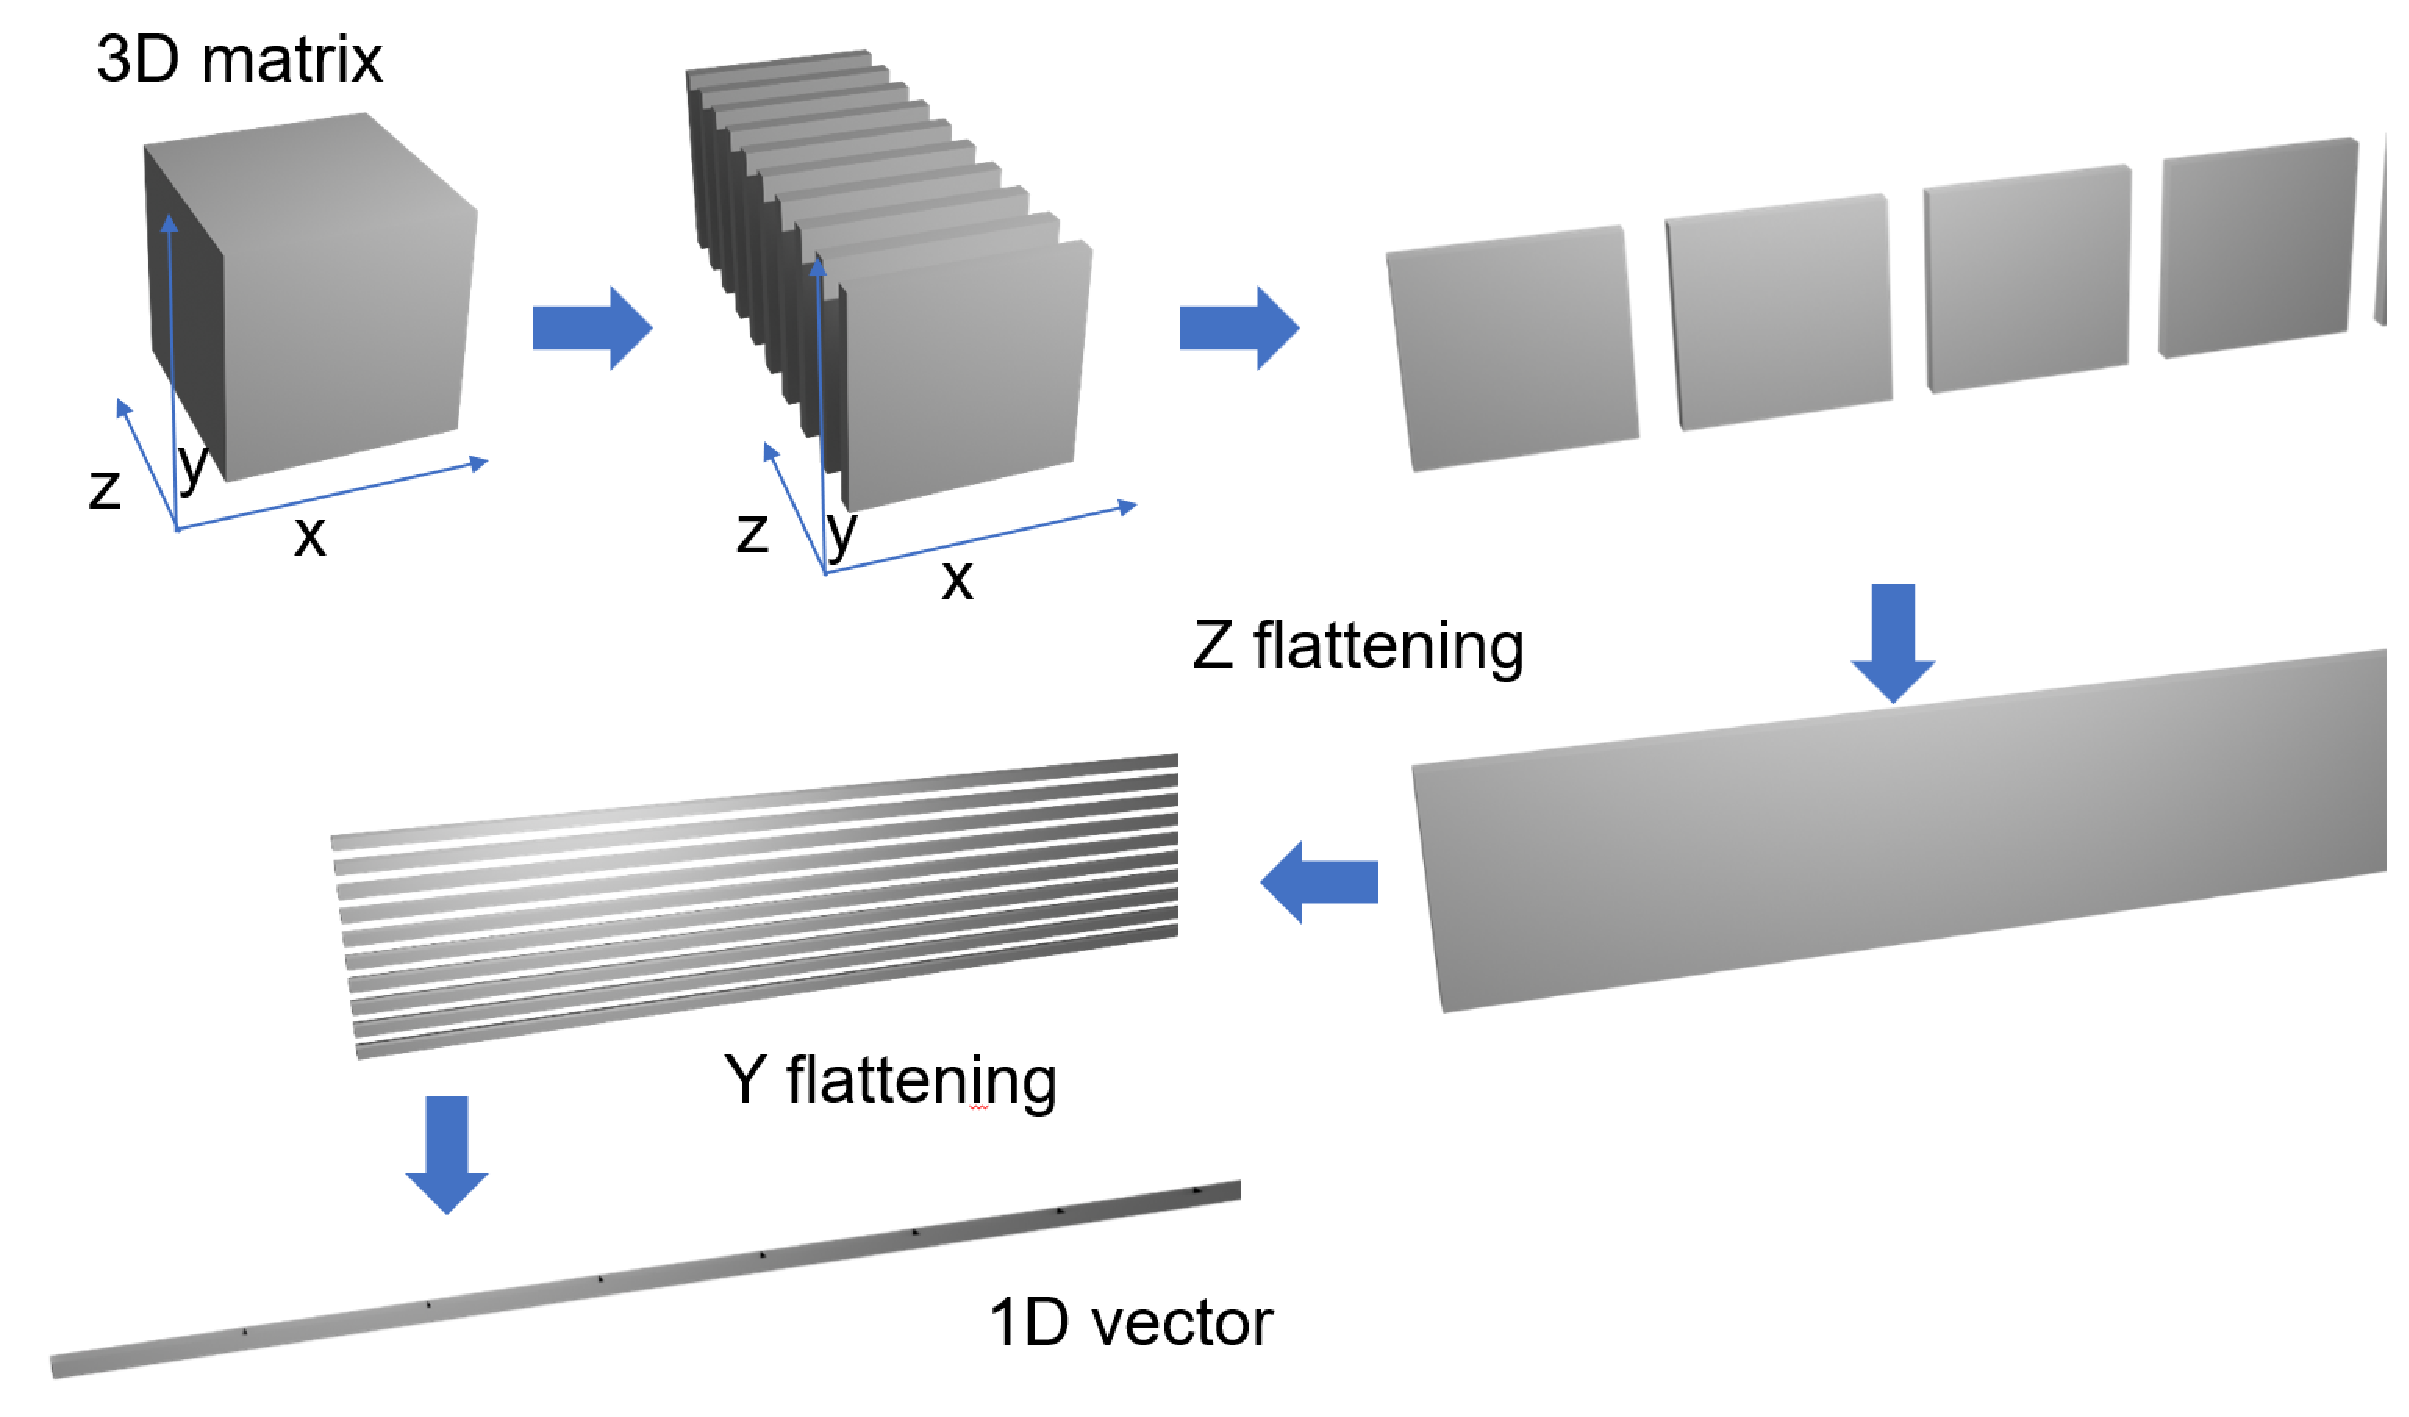
\includegraphics[width=\textwidth]{images/cracry/SVD_flattening.pdf}
  \hfill
  \caption{Schematic representation of the dimensional reduction process through which the isomorphous difference electron density maps are turned into one-dimensional vectors. An electron density map is a 3-D matrix, containing electron density values corresponding to points in the Unit-cell. To reduce it to a 1-D vector, the map is first sliced along the \(Z\) axis, and then all sheets created this way are stacked along the Y axis. after that, the long rectangle obtained is sliced along the \(Y\) axis, and all small vectors produced this way are stacked after the other to produce \(Vi\)}\label{fig:SVD_dimensional reduction}
\end{figure}


Because of that, all of the isomorphous \(F_{obs}(time\ point) - F_{obs}(dark)\) difference electron density maps deconvoluted had to be calculated at the same resolution so that the points in real space at which the electron density is sampled matched from one dataset to the other. The resolution of datasets in each series differs significantly (2.15 \AA\ for the ps-ns series, 2.42 \AA\ for the ns-\textmu s series). This is why the two series of isomorphous \(F_{obs}(time\ point) - F_{obs}(dark)\) difference electron density maps obtained during the ps-ns (SwissFEL) and ns-\textmu s (SACLA) experiments were analysed separately. This is also the reason for dropping the 10 ns time point dataset recorded in SACLA from the analysis of the ns - \textmu s series, as it contains the same information as the 10 ns dataset from SwissFEL and reaches a much lower resolution. 

The resolution was chosen as the lowest of each series. Difference maps were calculated for the entire asymmetric unit \footnote{It was suggested during the review process that the maps analysed should be limited to the region of interest. However the sequence of events produced by the SVD decomposition of local maps was the same, and therefore, we chose to apply the more straightforward global map approach.}. 

The isomorphous \(F_{obs}(time\ point) - F_{obs}(dark)\) difference electron density maps were calculated in Phenix \parencite{liebschnerMacromolecularStructureDetermination2019}, then converted from mtz to ccp4 format using the FFT implementation of the CCP4 suite \parencite{agirreCCP4SuiteIntegrative2023}. The maps were then opened within Python using the MRCfile package \parencite{burnleyRecentDevelopmentsCCPEM2017}.  The electron density values are stored in numpy arrays, then 'flattened' using the procedure described in Fig. \ref{fig:SVD_dimensional reduction}. The resulting input matrix is decomposed using the implementation of SVD in the DASK python package, which is more lightweight and able to deal with larger matrices without running out of memory. 

For each series, a matrix \(A\) was composed of the m successive Mi vectors (\(m = 9\) for the ps-ns series, and \(m = 4\) for the ns-\textmu s series). The \(m \times n\) matrix \(A\) was decomposed into the product of three matrices: \(A=U\times \Sigma \times V\). \(U\) is a \(n \times n\) unitary (square and of rank n) matrix. \(\Sigma\) is a \(n \times m\) rectangular matrix with singular values along the diagonal with decreasing importance from left to right. \(V\) is a unitary \(m \times m\) matrix. The columns of \(U\) are left Singular Vectors (lSV) representing time-independent structural elements in decreasing importance. The row i of \(V\) is a right singular vector (rSV), and represents the magnitude of each lSV in map E\textsubscript{i}. Each lSV vector can be transformed back into an electron density map lSV for visualization. Each map M\textsubscript{i} is a linear combination of time-independent maps lSV, whose scalar is the product of the singular values (diagonal terms in matrix \(\Sigma\)) and the corresponding magnitude (each coordinate rSV\textsubscript{i} in matrix V). 

Each lSV was examined in Coot \parencite{emsleyFeaturesDevelopmentCoot2010} to assess its structural significance. Based on this assessment and the significance of the time-dependent amplitude of the associated scalar, the first two lSVs were retained in the ps-ns series (Fig. \ref{fig:SwissFEL_SVD_MmCPDII}), as well as the first three lSVs in the ns-\textmu s series (Fig. \ref{fig:SwissFEL_SVD_MmCPDII}). All other lSVs are considered as noise features. Here, significant scalar magnitudes over time can be consulted in Fig. \ref{fig:SwissFEL_SVD_MmCPDII} (a) and Fig. \ref{fig:SACLA_SVD_MmCPDII} (a) for the ps-ns and ns-\textmu s series, respectively. Significant lSV time-independent maps for the ps-ns series are represented in Fig. \ref{fig:SwissFEL_SVD_MmCPDII} (b), and for the ns-\textmu s series in Fig. \ref{fig:SACLA_SVD_MmCPDII} (b) and (c). 

The original difference electron density map can be recomposed for any given time point 'i' by summing the structural components (lSV), scaled by their singular value (SV) and time factor (rSV) for that particular time point: \(Map_i=\sum_{j=1}^{n} rSV_{i,j} \times SV_{j} \times lSV_{j}\) where \(lSV_{i}\) comes from \(U\), \(SV_{i}\) comes from \(\sigma\) and \(rSV_{i,j}\) comes from \(V\) for that time-point and n is the number of rSV in \(V\). Notably, because scalars can adopt both positive and negative values, the polarity of the lSV map can switch according to its time-dependent scalar.

Individual components produced by the decomposition are \textbf{not necessarily} reaction intermediates. In the vast majority of cases, it is their combination which produces reaction intermediate states. 

This analysis was performed by in-house developed Python scripts (available at \url{https://github.com/ncara/SVD}), adapted from an implementation of SVD as a difference map noise filter \parencite{dodsUltrafastStructuralChanges2021}.

\subsection{Analysis} \label{sec:SVD_MmCPDII}

\subsubsection{CPD repair in three steps, visualized in the ns-ps TR-SFX series}
Despite originating from difference electron density maps calculated for the two monomers contained in the unit cell of \textit{Mm}CPDII, which contained noise-like peaks scattered around the unit cell, the signal of both lSV0 and lSV1 is limited to the region of the FAD and the CPD. This demonstrates the remarkable de-noising power of SVD analysis, which is already well documented \parencite{schmidtApplicationSingularValue2003, dodsUltrafastStructuralChanges2021, vallejosAppraisingProteinConformational2024}. 

rSV0 exhibits an approximately steady growth over the ns-ps time series (Fig. \ref{fig:SwissFEL_SVD_MmCPDII} (a)). In contrast, rSV1 exhibits 3 plateaus, from 100 to  650 ps, then \textasciitilde null from 1 to 3.35 ns, and finally negative from 6 ns onward. It appears that rSV0 represents the steady progress of the repair while rSV1 represents its modulation into three distinct steps. 

Accordingly, lSV0 presents a large negative electron density peak encompassing both the C5-C5' and one side of the C6-C6' bond while lSV1 features a positive peak on the C6-C6' and the bottom of the second base (Fig. \ref{fig:SwissFEL_SVD_MmCPDII} (b)), partially cancelling the signal contained in lSV1. Additionally, lSV0 presents a positive peak on the right side of the right base of the CPD, as well as negative peaks on the carbonyls of the left base of the CPD. 

Three steps can therefore be made out. From 100 to 650 ps, lSV2 cancels part of the signal of lSV0, and negative density is concentrated on the C5-C5' bond and the top part of the right base. At 100 ps, the CPD barely features any signal, as rSV0 is still weak, a negative electron density peak on the C5-C5' appears and increases in intensity with the growth of rSV0, showing that the transfer from the population from (T<>T)\textsuperscript{•-} to (T\_T)\textsuperscript{•-}. This validates that the initial electron transfer from the FAD to the CPD has happened, and that breakage of the C5-C5' bond occurs first, as proposed by ultrafast spectroscopy (discussed in Section \ref{sec:prior_MmCPDII}). But the information provided by TR-SFX here goes further: the left base of the CPD remains in place during this state (lSV1 contains positive peaks in the exact positions of the negative peaks of lSV0, on the carbonyls of the left base). The right base, however, is twisted, with its top part pushed away from the CPD while its bottom part is held in place by the intact C6-C6' bond. 

In the second step, only lSV0 is relevant: both C5-C5' and C6-C6' are covered by negative difference electron density. This suggests that C5-C5' and C6-C6' breakage has happened. Additionally, the long, vertical positive peak of lSV0 suggests that the right base of the CPD is no longer twisted, and is being separated from the left base (Fig. \ref{fig:SwissFEL_SVD_MmCPDII} (b)). This means that either species (T T)\textsuperscript{•-} or (T T) exist. 

In the last step, the polarity of lSV1 is reversed, and its signal now coherently builds into that of lSV0. The combined negative difference electron density on the C6-C6' bond and the lower region of the right base suggest that it is no longer twisted, having reached a planar conformation, positioned on the left side of the elongated positive peak of lSV0 (Fig. \ref{fig:SwissFEL_SVD_MmCPDII} (b)). Interestingly, the negative peaks on the carbonyls of the left base suggest that they match the movement of the first base and that they both engage in planar stacking. This element, as well as the loss of the twisted geometry of the right base, means that the electron transfer has happened and that the right base is no longer an anionic radical, allowing it to stack with the left base. 

\begin{figure}[H]
  \centering
  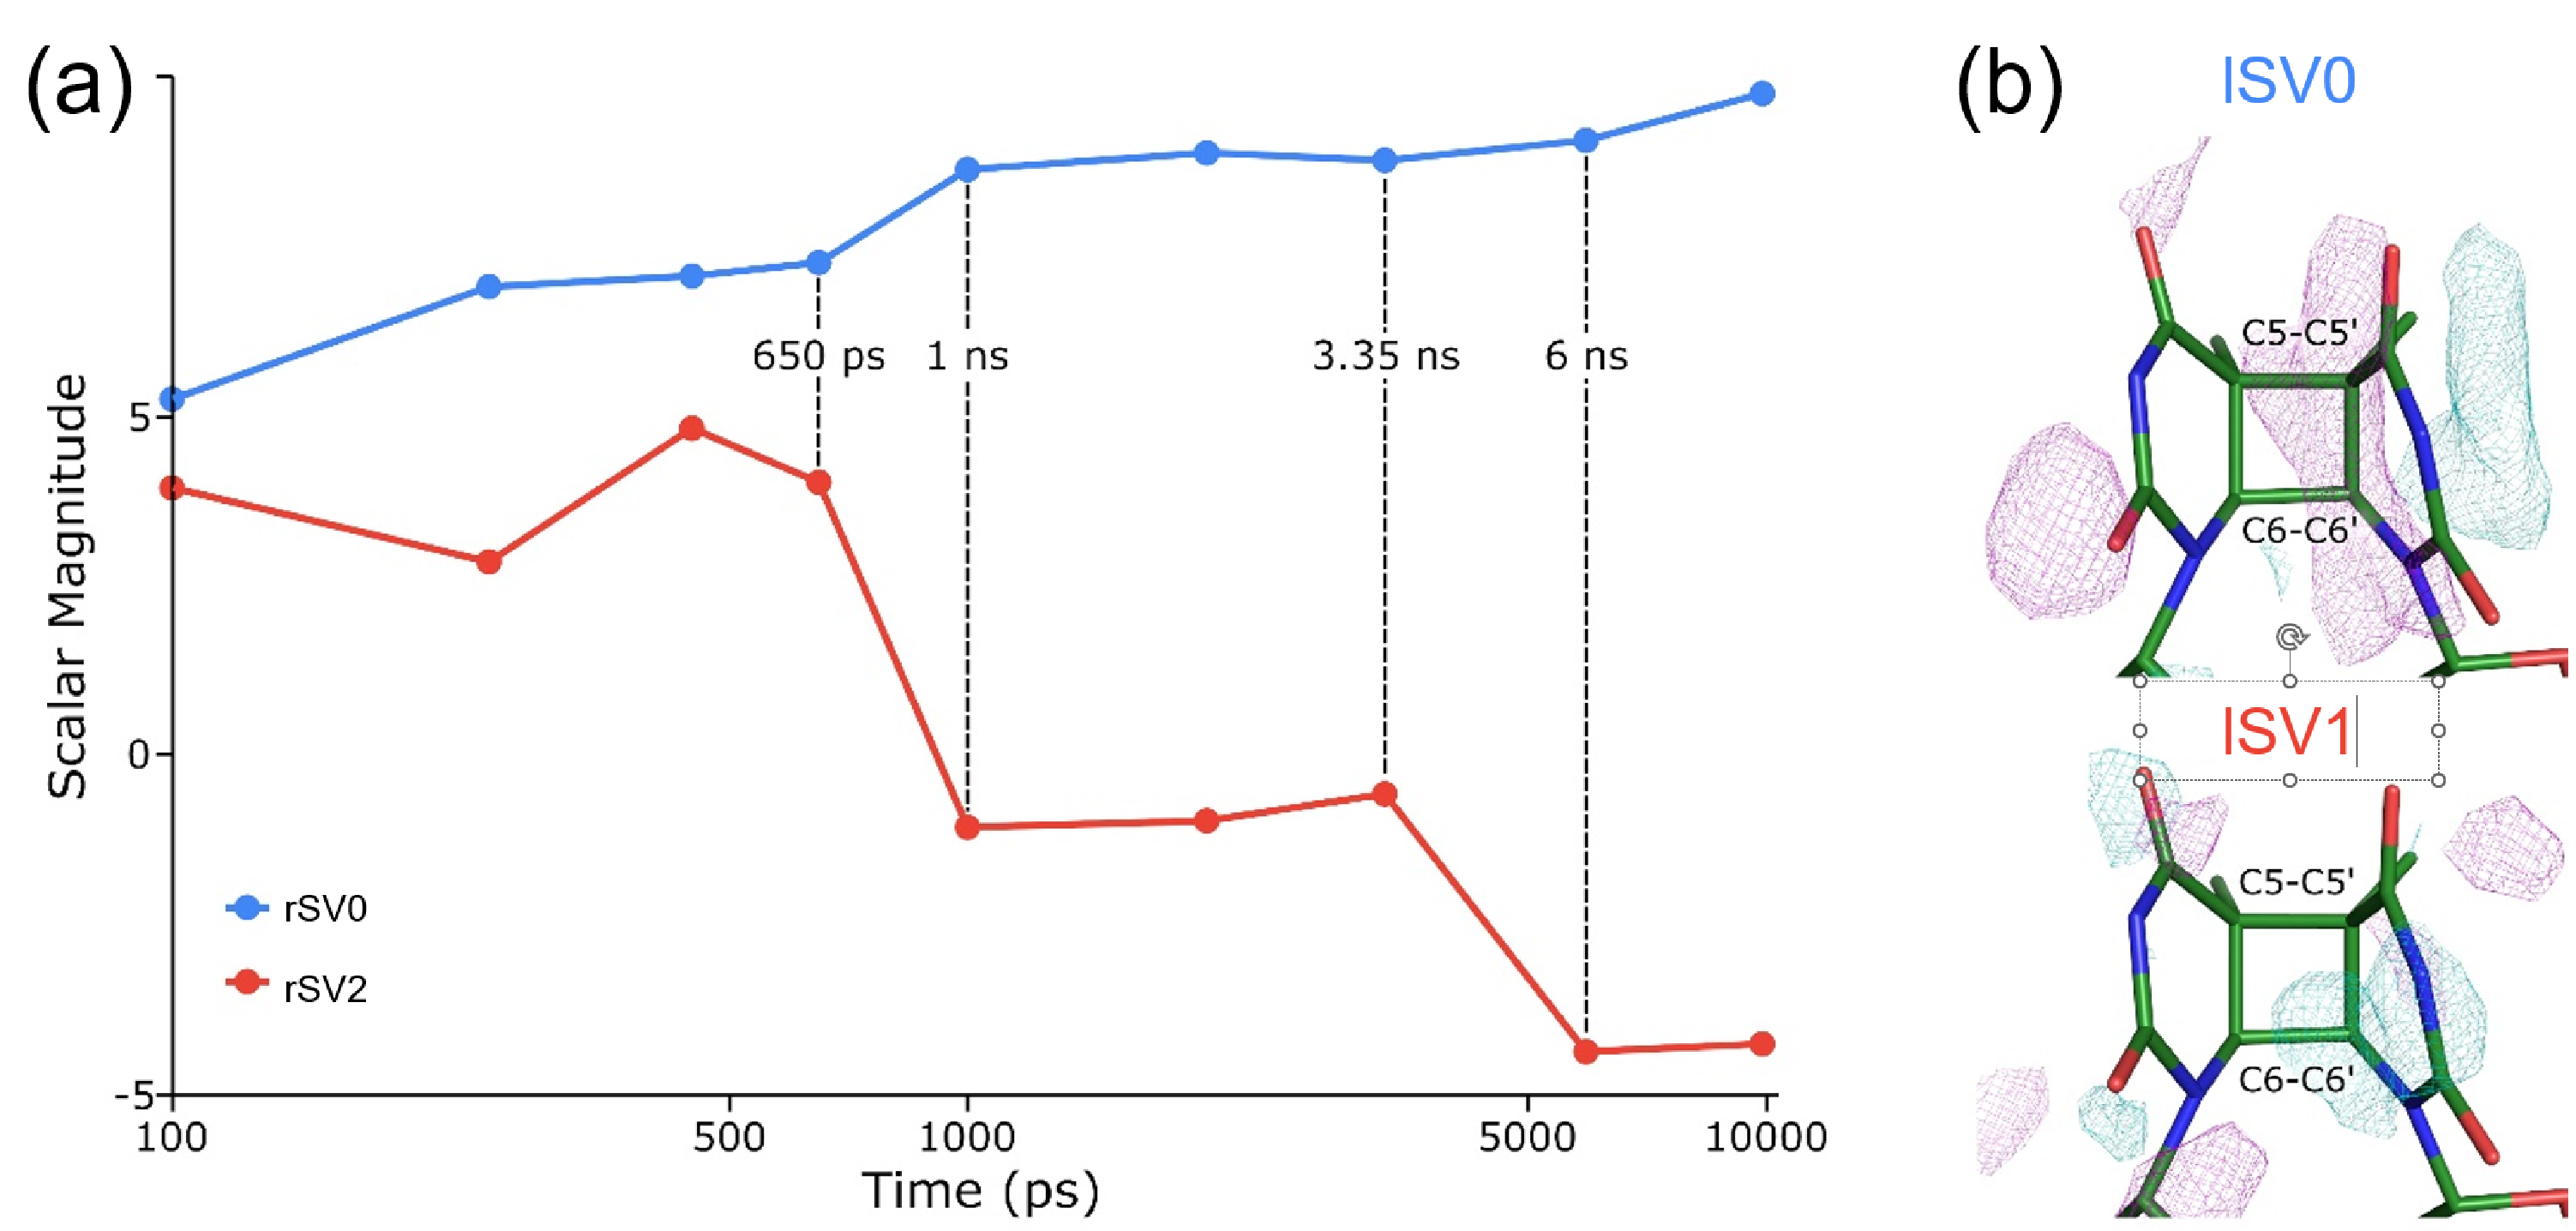
\includegraphics[width=\textwidth]{images/cracry/SwissFEL_SVD.pdf}
  \hfill
  \caption{Deconvolution of the first series of maps (ps - ns) collected at SwissFEL. (a) Time-dependent scalar (rSV) of the two relevant components for that series (SV0 in blue, SV1 in red) plotted over time. Three broad stages can be distinguished: SV0 and SV1 are positive, from 100 to 650 ps; SV0 is positive and SV1 is \textasciitilde null, from 1 to 3.35 ns and SV0 is positive and SV1 is negative, from 6ns onward. (b) Time-independent structural elements (lSV) of the two most prominent features. lSV0 features a negative peak encompassing both the C5-C5' and C6-C6' bonds and spanning over the left base of the CPD, as well as a positive peak on the side of the left base. lSV1 features a positive peak on the C6-C6' bond and the lower portion of the second base of the CPD. Reproduced from the supplementary material of \cite{maestre-reynaVisualizingDNARepair2023a}}\label{fig:SwissFEL_SVD_MmCPDII}
\end{figure}

\subsubsection{DNA release and annealing visualised by the ns-\textmu s TR-SFX series}

Whereas the ps-ns series was dominated by two components, the ns-\textmu s series presented three significant components (Fig. \ref{fig:SACLA_SVD_MmCPDII}). As was the case for the lSVs of the first series, both lSV0 and lSV2 contain signal restricted to the CPD and FAD region (Fig. \ref{fig:SACLA_SVD_MmCPDII} (c)). However, the second time-independent structural component, lSV1, contains negative difference electron density spanning all over the damaged strand of the DNA fragment (purple in Fig. \ref{fig:SACLA_SVD_MmCPDII} (c)). 

Between 100 ns and  500 ns, rSV0 is the strongest scalar (in absolute value), while rSV2 is negligible and rSV1 is moderate but negative (Fig. \ref{fig:SACLA_SVD_MmCPDII} (a)). At 25 \textmu s, rSV0 and  rSV1 are positive, while the rSV2 scalar is negative. The summation of the signal contained in lSV1 and lSV3 results in a pronounced signal around the CPD, while the relative weakness of rSV2 indicates that the rest of the DNA strand has not been strongly affected yet. Finally, at 200 \textmu s, rSV1 has overtaken even rSV0 as the dominant vector (Fig. \ref{fig:SACLA_SVD_MmCPDII} (a)), resulting in an intense signal around the DNA. The 'pendulum swing' (positive, negative, and positive again) behaviour of rSV3 suggests that it is a modulating factor, while both rSV0 and rSV1 display clear trends (decreasing and increasing from 500 ns on, respectively).

lSV0 contains mostly negative difference electron density, spanning over the entire cyclobutane portion of the CPD, as well as the lower part of the right base, and the carbonyl of the left base (Fig. \ref{fig:SACLA_SVD_MmCPDII} (b)). lSV1 contains negative peaks over the position of the bases, and lSV2 contains one large negative electron density peak spanning over the C5-C5' and C6-C6' bonds, as well as the top carbonyl of the right base. The electron density peaks of lSV0 and lSV1 do not overlap, which indicates they complement each other. However, the signal of lSV3 overlaps with that of lSV0, which confirms that lSV3 is a modulating factor of lSV0.

Again, three distinct states can be distinguished: between 100 and 500 ns, the negative electron density peak contained in lSV0 coupled by the positive peaks produced by the reversed polarity of lSV1 (Fig. \ref{fig:SACLA_SVD_MmCPDII} (b)), reproduce the signal observed at 10 ns, the end of the SwissFEL series. This indicates that the bases are lingering in their stacked conformation, similar to what was observed at the end of the first series. 

At 25 \textmu s, lSV0 decreases in intensity and is partially cancelled by a negative lSV2, and completed by a weakly positive lSV1. The resulting pattern is a thin positive peak, diagonally crossing the cyclobutane in the same position as the negative peak of lSV2 (Fig. \ref{fig:SACLA_SVD_MmCPDII} (b)). It is surrounded on both sides by negative peaks corresponding to the margin of the main peak of lSV0 and negative peaks of lSV1. This corresponds to an intermediate in the flip-back movement of the bases, where the former left base of the CPD is now diagonally crossing the former position of the cyclobutane, and the right base is lower, re-integrating into the strand. This intermediate was refined via structure factor extrapolation and is presented in the main text of \cite{maestre-reynaVisualizingDNARepair2023a} (Fig. \ref{fig:CraCRY_Cter} D).

Finally, at 200 \textmu s, the leading signal is lSV1, indicating that the damaged strand of DNA is no longer twisted to integrate the CPD into the annealing bubble of the photolyase (evidenced by the negative electron density visible on the DNA strand in Fig. \ref{fig:SACLA_SVD_MmCPDII} (c)). It is completed by the global negative electron density from positive lSV0 and lSV1, covering the entire position formerly occupied by the CPD. 

\begin{figure}[H]
  \centering
  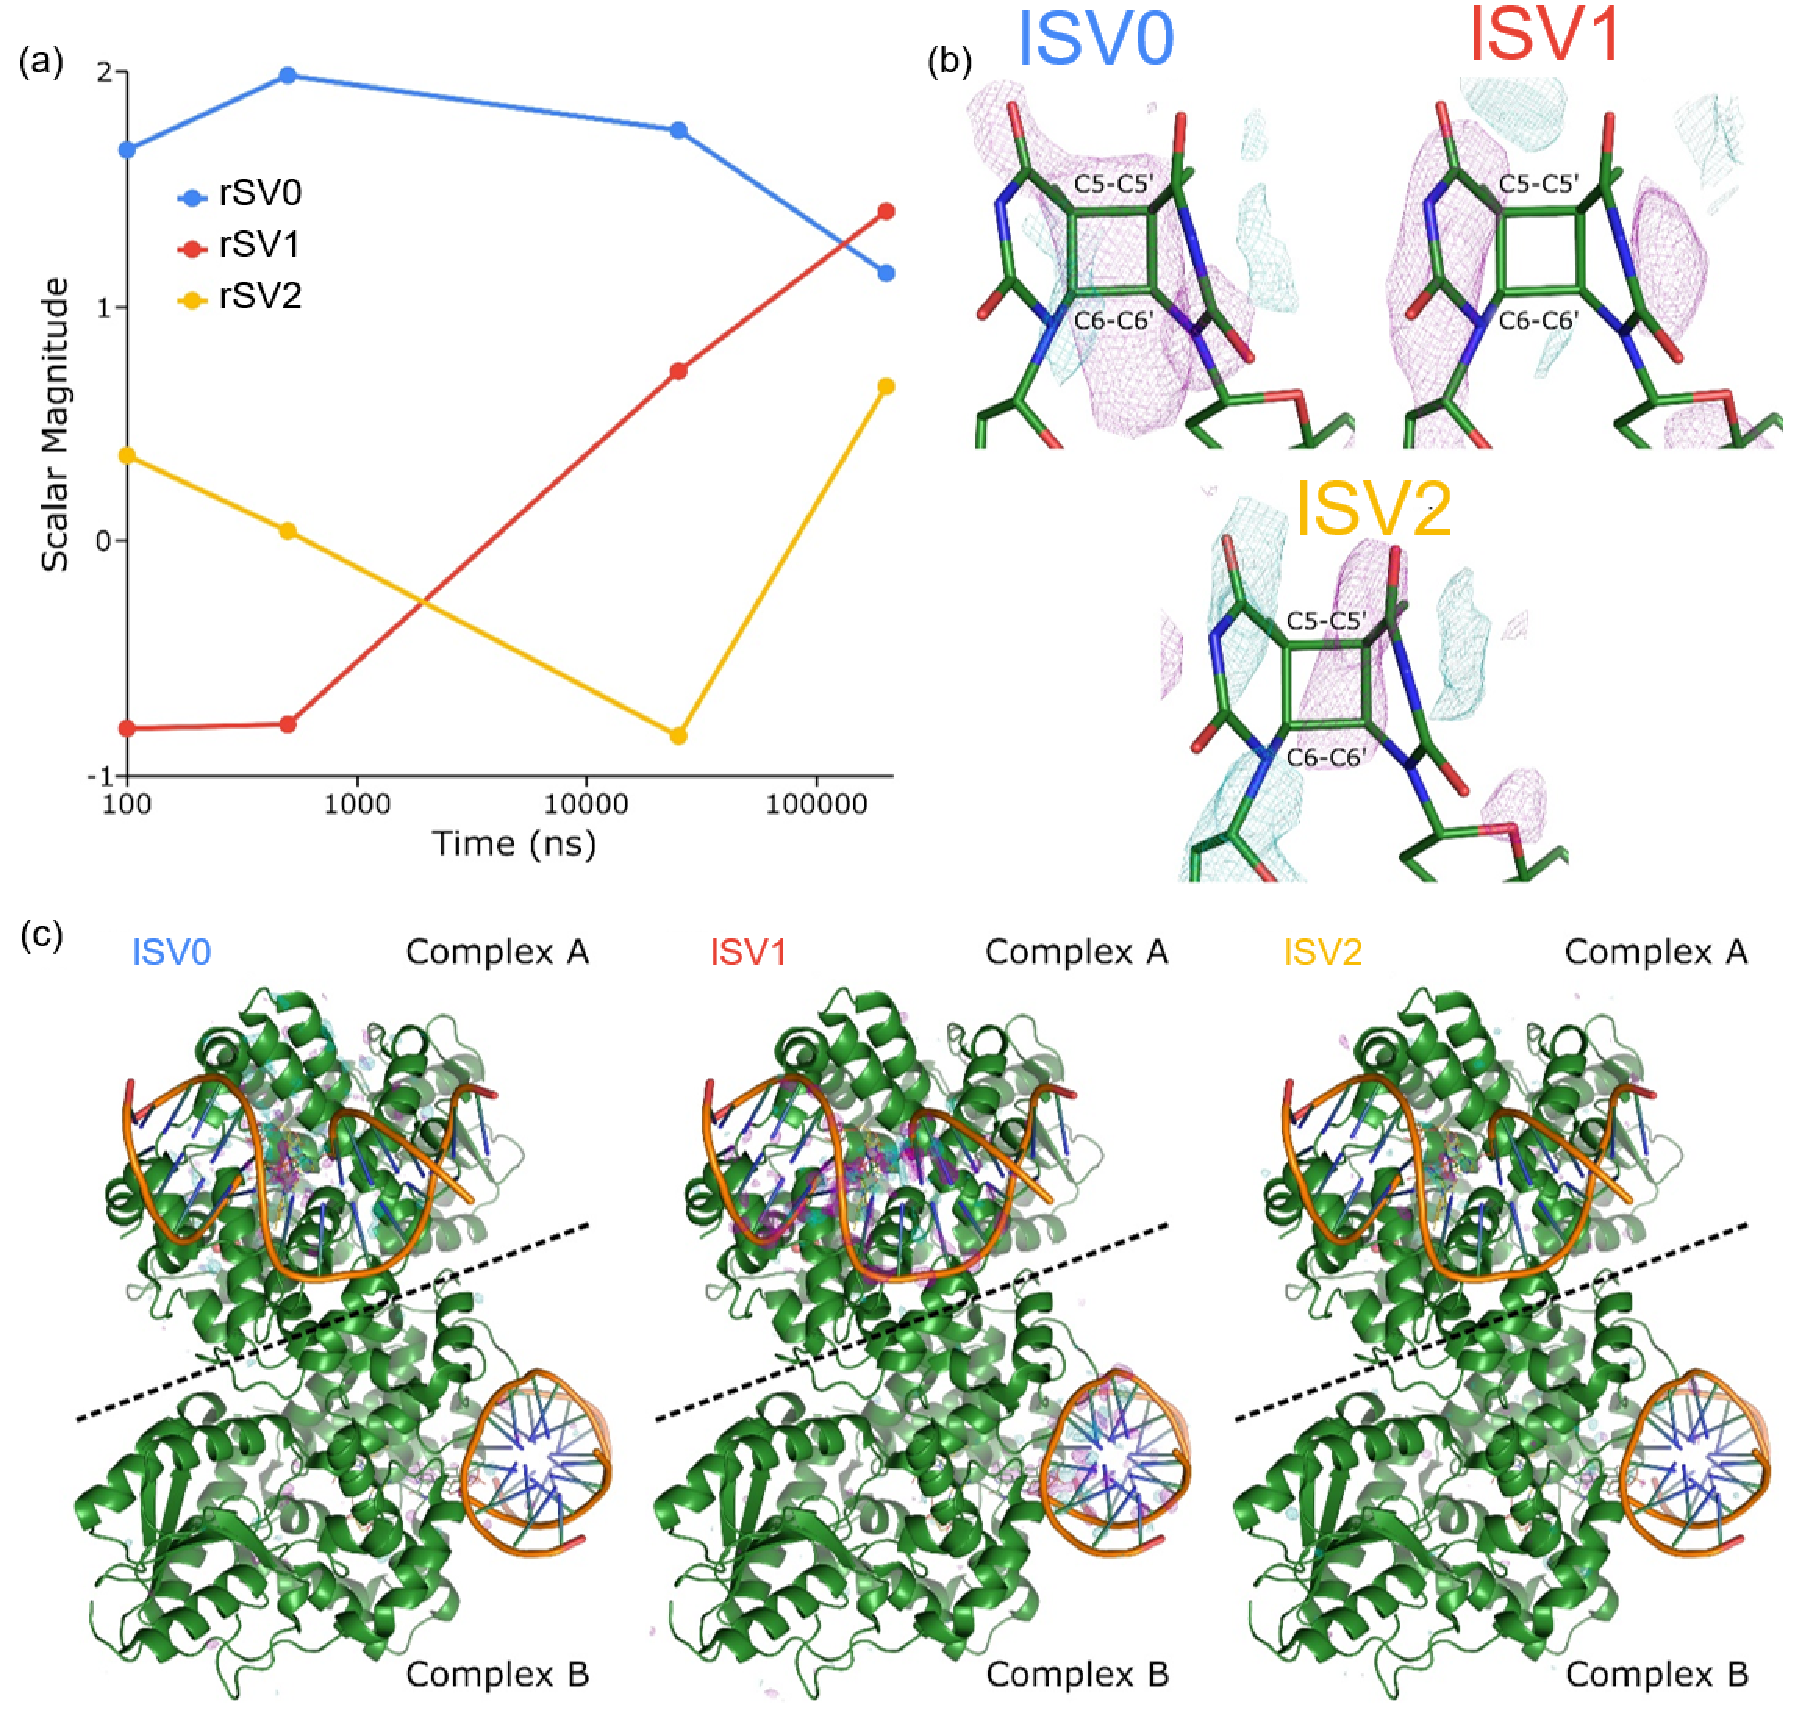
\includegraphics[width=\textwidth]{images/cracry/SACLA_SVD.pdf}
  \hfill
  \caption{Deconvolution of the second series of maps (ns - \textmu s) collected at SACLA. (a) Time-dependent scalar (rSV) of the three relevant components for that series (SV0 in blue, SV1 in red and SV2 in yellow) plotted over time. Three broad stages can be distinguished: SV0 and SV1 are positive, from 100 to 500 ns; SV0 is positive, SV1 is negative and SV2 is \textasciitilde null, at 25 \textmu s, SV0 is positive, SV1 is \textasciitilde null and SV2 is negative, finally, at 200 \textmu s all three lSV are positive and lSV1 overtakes both lSV 0 and lSV2. (b) CPD-centered view of the time-independent structural elements (lSV) of the three most prominent features in the decomposition. lSV0 features a negative peak encompassing the entire cyclobutane, and lSV1 contains negative peaks over each side of the CPD. lSV2 features a negative peak spanning both the C5-C5' and C6-C5' bonds as well as the carbonyl on top of the second base. It also contains positive beaks on the side of the first base. (c) overview of lSV0, lSV1 and lSV2 over the entire unit cell, evidencing that the signal is concentrated on the CPD and the FAD cofactor for lSV1 and lSV2, while lSV1 also features negative peaks over the entire damaged region of the damaged strand in the DNA fragment. Reproduced from the supplementary material of \cite{maestre-reynaVisualizingDNARepair2023a}}\label{fig:SACLA_SVD_MmCPDII}
\end{figure}

Here, SVD analysis was able to validate that the rupture of the C5-C5' bond precedes that of C6-C6' bond. Further, it allowed us to identify a novel long-lived intermediate where both repaired, neutral bases are engaged in co-planar stacking. 

It was also able to identify that the conformational mechanism underlying the release of the DNA strand after repair happens via a three-step mechanism, as well as suggest the structures of the steps (stacking, flip-back, release). 

The presentation of the analysis here focused on the CPD, but the SVD analysis was able to correlate the conformational changes of the FAD with that of the CPD and link the conformation of key amino acids in the CPD pocket with the stabilisation of the intermediates of DNA release identified. 

SVD analysis constitutes a scaffold on which a kinetic model can be built. Because they can switch polarity, the rSV are difficult to translate to occupancies of an intermediate state. However, they can be used to validate the trends identified by integrating difference density. Indeed, difference density integration can produce drastically different results depending on the size and the shape of the integration volume, and validating it with a more global, less subjective method proved important to convince readers of the validity of the model we proposed. 

\chapter{The early steps in signalling from a bifunctional cryptochrome, traced by TR-SFX and TR-\textit{ic}OS}\label{chap:CraCRY_TR-SFX_1}


\noindent  Only my contributions to the study, put into context, will be discussed in this chapter.
\vspace{10mm}

In addition to the study of DNA repair by \textit{Mm}CPDII, the collaboration network described in Section \ref{sec:prior_MmCPDII} studied the photoreaction of the novel animal-like cryptochrome of \textit{Chlamydomonas reinhardtii} (CraCRY) described in Section \ref{sec:cryptochrome_families}.

\section{The animal-like cryptochrome: multi-functionality governed by the redox state of the flavin cofactor}

As mentioned in Section \ref{sec:cryptochrome_families}, cryptochromes are flavin-binding, signalling proteins. They belong to the same overarching family as photolyases and evolved from 6-4 photolyases as animal-like (animal-like cryptochrome) and Class II CPD photolyases as plant-like (pCRY, CryP) and DASH-type CRYs \parencite{meiEvolutionaryHistoryPhotolyase2015}. 

While photolyases catalyze light-driven DNA repair \parencite{sancarMechanismsDNARepair2016, essenLightdrivenDNARepair2006}, CRYs modulate plant growth, regulate circadian rhythms \parencite{chavesCryptochromesBlueLight2011}, and act even as magnetoreceptors \parencite{ritzResonanceEffectsIndicate2004, horeRadicalPairMechanismMagnetoreception2016, xuMagneticSensitivityCryptochrome2021}. As evolutionary transitional forms, some CRYs like the animal-like cryptochrome from \textit{Chlamydomonas reinhardtii} (CraCRY) act as photoreceptors \parencite{beelFlavinBindingCryptochrome2012, petersenWorldAlgaeReveals2021, zouAnimalCryptochromeControlsChlamydomonas2017} and have retained their DNA repair capabilities \parencite{franzStructureBifunctionalCryptochrome2018}. 

The biological function performed by photoreceptor cryptochromes depends on light-driven electron transfer to their FAD chromophore \parencite{kavakliPhotolyaseCryptochromeFamily2017, chavesCryptochromesBlueLight2011, brettelReactionMechanismsDNA2010}. The electron transfer pathway leading to the semi-reduced FAD cofactor in CraCRY is presented in Fig. \ref{fig:CraCRY_photoreaction}. CraCRY uses a tetrad of four aromatic residues (Fig. \ref{fig:CraCRY_photoreaction} (b), \cite{franzStructureBifunctionalCryptochrome2018, nohrExtendedElectronTransferAnimal2016,oldemeyerEssentialRoleUnusually2016}) for FAD photoreduction and subsequent formation of the signalling-relevant FADH\textsuperscript{•} state \parencite{beelFlavinBindingCryptochrome2012}, as opposed to the triad of residues used by the vast majority of cryptochromes and photolyases (Fig. \ref{fig:transferchain}). Like in other PCSf members of the animal-like cryptochrome/6-4 photolyase branch \parencite{martinUltrafastFlavinPhotoreduction2017,timmerTrackingElectronTransfer2023}, these residues (CraCRY: W399, W376, W322 visible in green and Y373 coloured in teal in Fig. \ref{fig:CraCRY_photoreaction} (b)) form a 22 \AA\ long electron transfer pathway from the surface of the C-terminal photolyase homology region (PHr, corresponding to the combined pink and blue subdomains, as well as their linkers in Fig. \ref{fig:PCSF} (b), \cite{meiEvolutionaryHistoryPhotolyase2015}) domain towards the FAD chromophore (coloured yellow in Fig. \ref{fig:CraCRY_photoreaction} (b)). 

Ultrafast spectroscopic studies on CraCRY showed that photoexcited FAD\(^\ast\) abstracts an electron from its neighbour within <0.4 ps, W399 (Fig. \ref{fig:CraCRY_photoreaction} (a), \cite{lacombatUltrafastOxidationTyrosine2019}). The resulting electron-hole at W399•+ (red in Fig. \ref{fig:CraCRY_photoreaction} (b)) then hops via aromatic residues of the electron transfer pathway towards Y373 (green in Fig. \ref{fig:CraCRY_photoreaction} (b)), with the slowest step being proton-coupled electron transfer (PCET, Fig. \ref{fig:CraCRY_photoreaction} (a)). PCET (\texttau=0.8 ns, Fig. \ref{fig:CraCRY_photoreaction} (a)) involves electron transfer between W322 and Y373 and concomitant PT within the hydrogen-bonded D321/Y373 pair (both green in Fig. \ref{fig:CraCRY_photoreaction} (b),\cite{lacombatUltrafastOxidationTyrosine2019}).  Thus, a FAD\textsuperscript{•–}/Y373\textsuperscript{•} radical pair is formed in less than a nanosecond, via an electron chain a full 22 \AA\ long. 

\begin{figure}[H]
  \centering
  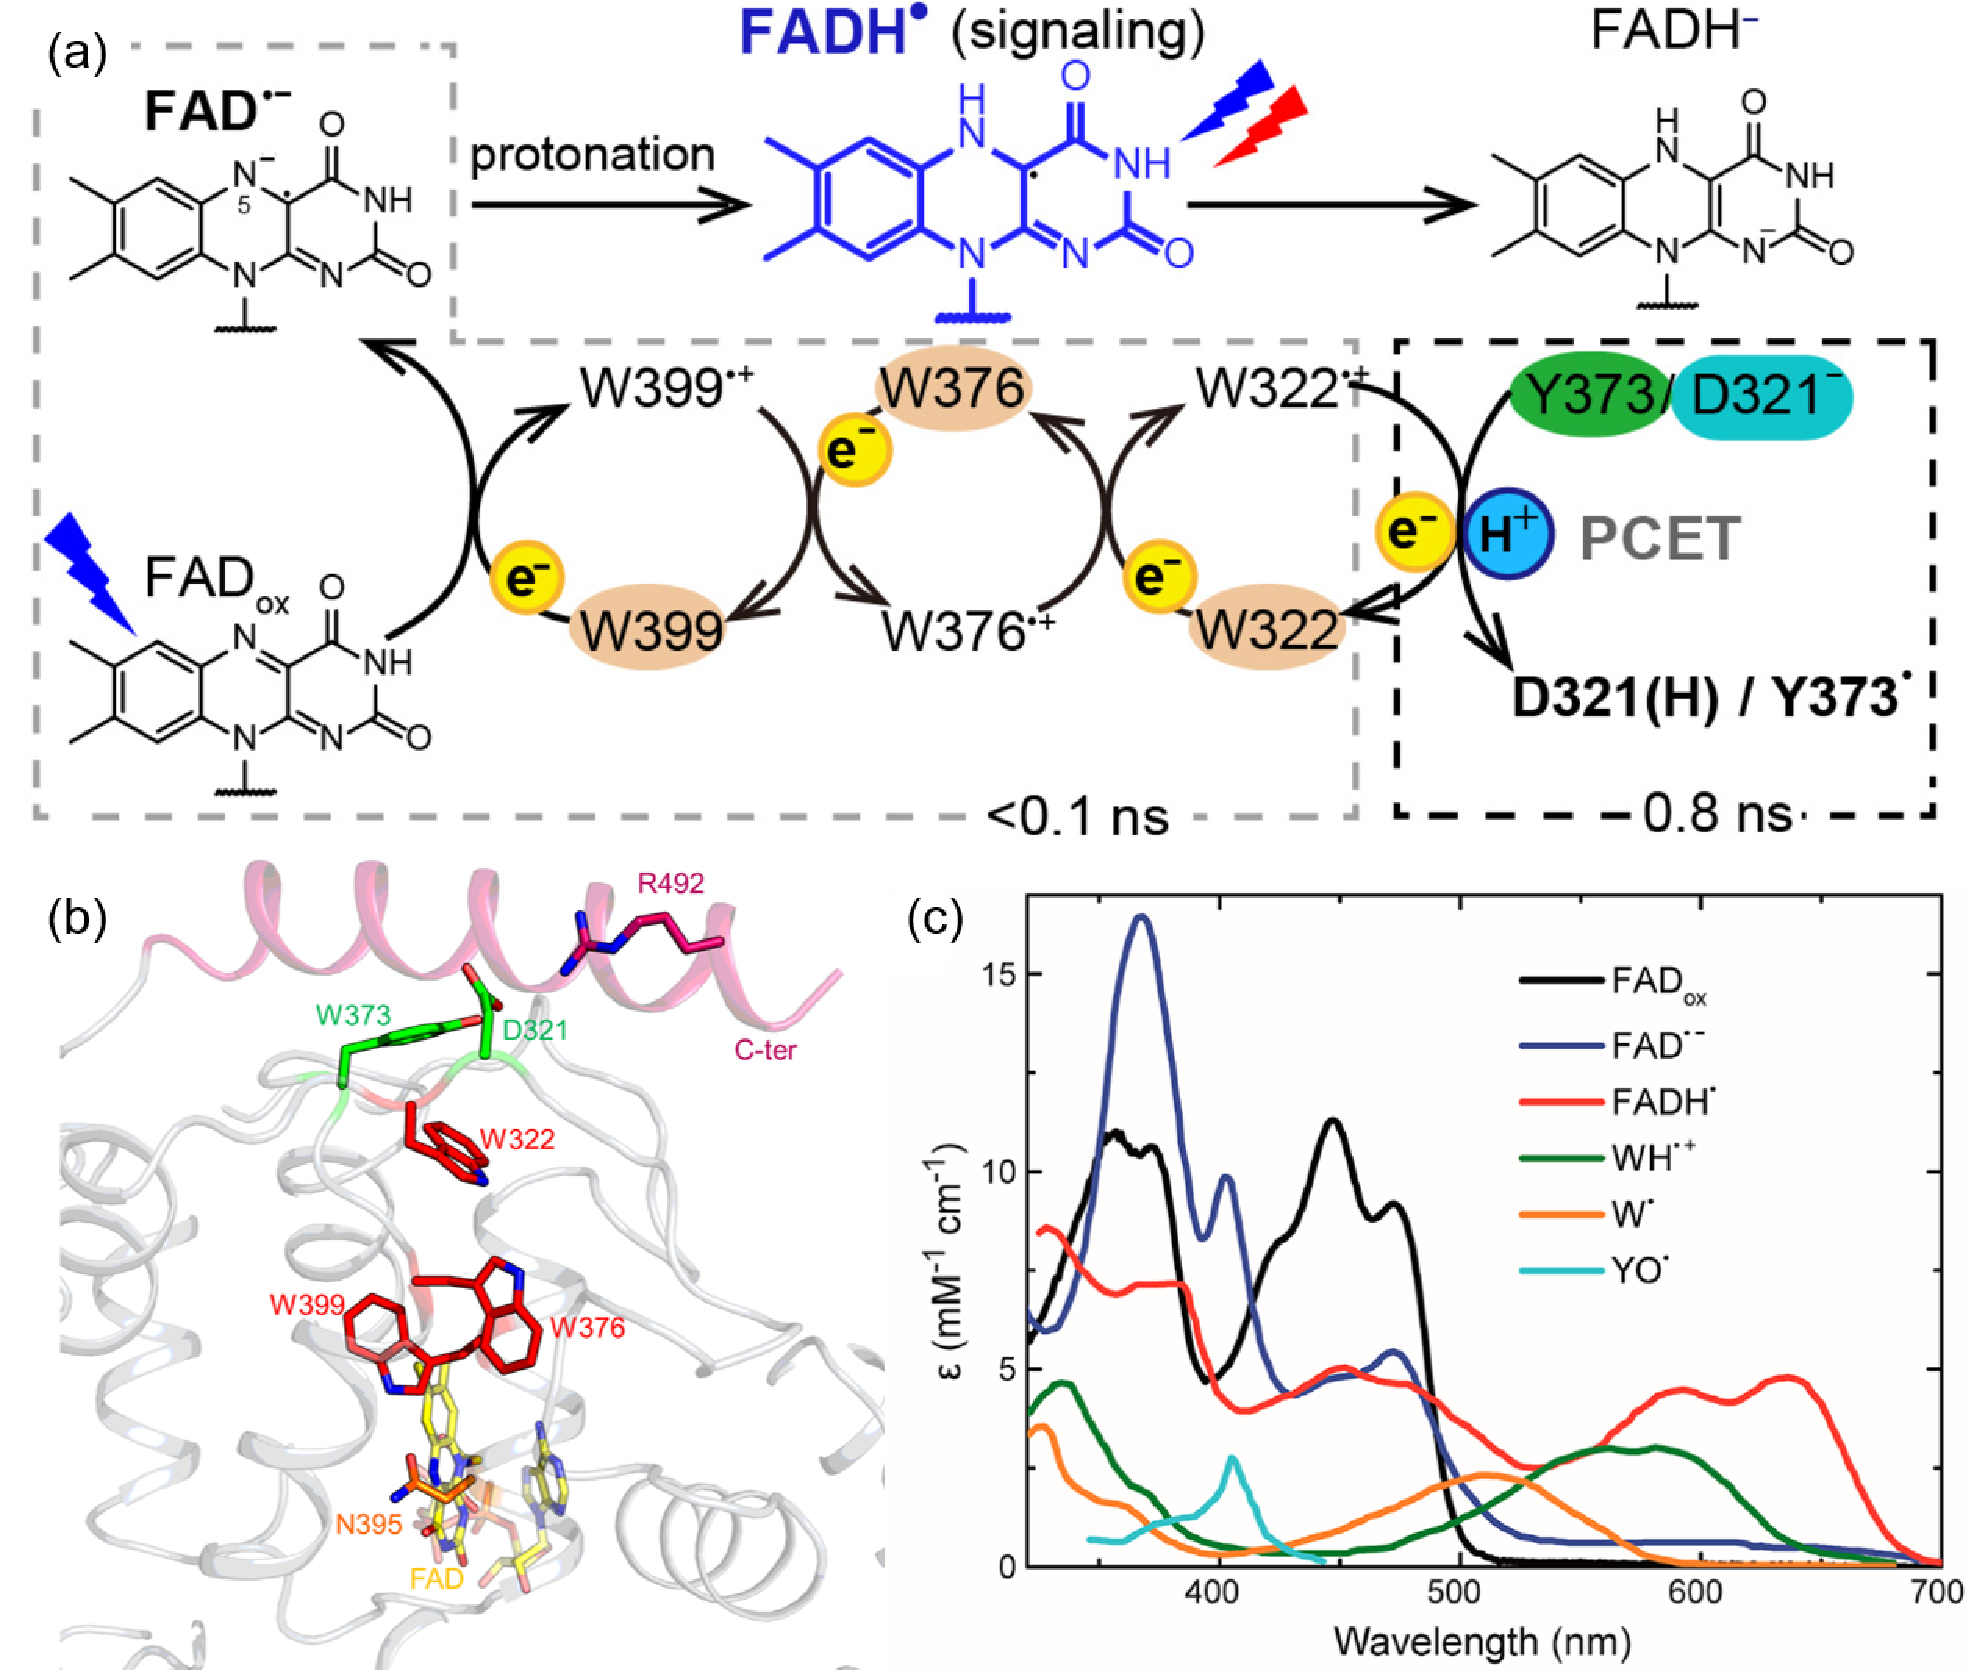
\includegraphics[width=\textwidth]{images/cracry/Photocycle_CraCRY.pdf}
  \hfill
  \caption{Photoreaction of CraCRY. (a) Schematic representation of followed by CraCRY for its different functions. FAD\textsuperscript{ox} photoreduction generates the FAD\textsuperscript{•–}/Y373\textsuperscript{•} radical pair by electron transfer from Y373 (dashed boxes) within less than one nanosecond, whereas PT to FAD\textsuperscript{•–} (top) is pH-dependent and proceeds slower in the sub-second time range \parencite{lacombatUltrafastOxidationTyrosine2019}. A further reduction to FADH– allows CraCRY to act as (6-4) photolyase \parencite{franzStructureBifunctionalCryptochrome2018}. (b) Overview of the key regions of CraCRY in the TR-SFX series. The FAD cofactor (yellow) is linked to the \textalpha22 C-terminal helix (purple) by a tetrad of amino acids responsible for the electron transfer: the original tryptophan triad (W399, W376 and W222, red) and the final tyrosine (Y373, green). The proton donor of the tyrosine for PCET (D321, green) is involved in a network of salt bridges stabilising \textalpha22 via R392 (purple). A conserved asparagine stabilises the radical FAD (N395, orange). (c) AS signatures of all of the FAD cofactor redox states, obtained as steady spectra. (c) is reproduced from \parencite{lacombatUltrafastOxidationTyrosine2019}.}\label{fig:CraCRY_photoreaction}
\end{figure}

% With a sequence identity of 61\% for the PHr domain, CraCRY is highly related to  that of the European robin (\textit{Erithaculus rubecula}) CRY4a. The latter is receptive to the Earth’s magnetic field \parencite{xuMagneticSensitivityCryptochrome2021} using a spin-correlated radical pair  \parencite{ritzModelPhotoreceptorBasedMagnetoreception2000,ritzResonanceEffectsIndicate2004,horeRadicalPairMechanismMagnetoreception2016} and may hence be the bird’s compass for migration. In the following, we used our CraCRY model to show how photoreduction of an animal-like cryptochrome causes structural changes in its C-terminal region 22 \AA\ away from its FAD chromophore to foster potential downstream signalling. 
% As weak magnetic field sensitivity of RPs depends crucially on the lifetimes of their spin-correlation in the \textmu s range \parencite{horeRadicalPairMechanismMagnetoreception2016,rodgersChemicalMagnetoreceptionBirds2009}, the structural events occurring in CraCRY and affecting the lifetime of the radical pair are particularly important. 

The lifetime of the radical pair in CraCRY directly depends on whether or not fast non-productive recombination of the FAD\textsuperscript{•–}/Y373\textsuperscript{•} radical pair can happen \parencite{lacombatUltrafastOxidationTyrosine2019}. In CraCRY, the radical FAD\textsuperscript{•–} is eventually protonated, which prevents non-productive recombination and greatly extends the lifetime of the radical pair \parencite{lacombatUltrafastOxidationTyrosine2019}. However, CraCRY structures of all redox states lack such a protonation pathway leading from solvent to the flavin cofactor’s N5 nitrogen. This occlusion of FAD’s N5 from solvent access is not only found for CraCRY but also a general feature of structurally characterized members of the cryptochrome/photolyase family. 

Consequently, the TR-SFX experiment aimed at identifying structural events altering the lifetime of the radical pair, and chief among them, the protonation of the FAD\textsuperscript{•–} into FADH\textsuperscript{•}. To address these issues, a series of 18 TR-SFX time-points (10, 30, 100, 300 ns; 1, 10, 30, 100, 300 \textmu s; 1, 7, 33, 66, 100, 133, 166, 200, 233 ms) was recorded with a pump-probe scheme, using a 3 ns laser pulse at a wavelength of 450 nm as a pump at the SACLA XFEL, in Japan. Given the sub-ns rates for photochemical and electron transfer reactions \parencite{lacombatUltrafastOxidationTyrosine2019}, this series focused on achieving TR-SFX snapshots of the conformational changes of CraCRY after having accomplished FAD\textsuperscript{•-}/Y373\textsuperscript{•} radical pair formation.

When analyzing snapshots evolving from the radical pair via difference electron density maps, we observed time-dependent differences in two major regions (represented in Fig. \ref{fig:CraCRY_photoreaction} (b)). \textbf{(1)} N395 at the FAD binding site (respectively coloured orange and yellow in Fig. \ref{fig:CraCRY_photoreaction} (b), with a close-up view of the features represented in Fig. \ref{fig:CraCRY_protonation} (a), (b) and (c)), and \textbf{(2)} the C-terminal helix \textalpha22 including its interface to the PHr domain (represented in green in Fig. \ref{fig:CraCRY_photoreaction}, a close-up view is presented in Fig. \ref{fig:CraCRY_Cter}). Each of these regions will be addressed separately.

\subsection{The binding pocket of the FAD cofactor adapts to protonation}

Peaks around  isoalloxazine moiety, indicating that it bends upon formation of the FAD\textsuperscript{•-} species, appear in early difference electron density maps (10ns-dark) (Fig. \ref{fig:CraCRY_protonation} (a)). The strongest difference in electron density peaks appearing in the flavin binding pocket during the entire time course is located around the carboxamide head of N395. As suggested by previous reports for the conserved counterparts of N395 in other cryptochromes and photolyases \parencite{maestre-reynaSerialCrystallographyCaptures2022,wijayaSingleHydrogenBond2016,iwataKeyDynamicsConserved2010}, N395 is rotated by 90 \degree at the 10 ns mark, stabilising the anionic FAD radical. 

After the initial inspection of the difference electron density maps, two regions of the time course during which the protonation of the FAD\textsuperscript{•–} into FADH\textsuperscript{•} could have happened were identified. The first of these regions is from 3 and 10 \textmu s, when the strain on the FAD relaxes, as evidenced by the disappearance of the difference electron density peaks around the isoalloxazine ring (Fig. \ref{fig:CraCRY_protonation} (b)), and the difference electron density pattern around N395 transitions from a four leaved-clover to a three-leaved clover shape, suggesting that N395 is more dynamic. 

The second of these regions is from 7 to 100 ms, when the difference electron density pattern around N395 evolves yet again into a stronger pair of peaks (positive and negative), closer to the N\textdelta2 atom. This suggests that N395 has moved somewhere between the 90 \degree clockwise rotated position exhibited at the beginning of the series (Fig. \ref{fig:CraCRY_protonation} (a)), and the position of the N395 in the oxidised dark state. 

\begin{figure}[H]
  \centering
  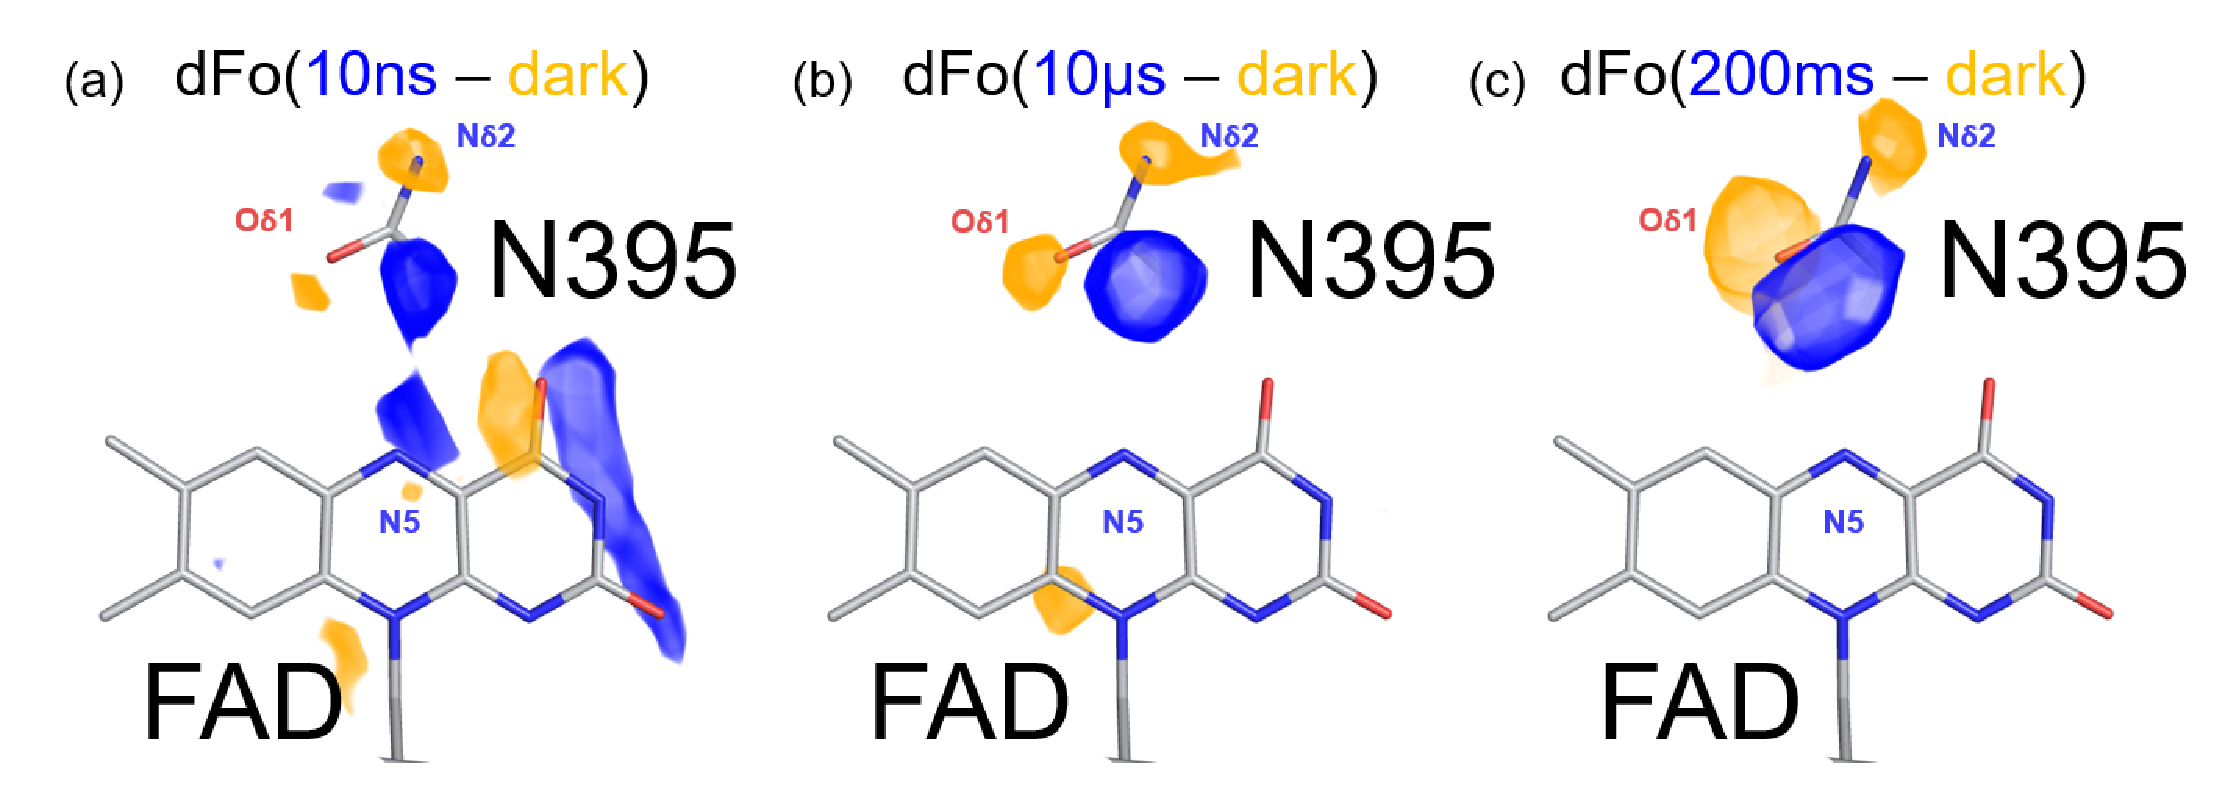
\includegraphics[width=\textwidth]{images/cracry/CraCRY_protonation.pdf}
  \hfill
  \caption{Isomorphous \(F_{obs}(time\ point) - F_{obs}(dark)\) electron density maps features around the FAD and N395 contoured at 3.5 \textsigma level and overlaid on the oxidised state model (negative electron density is coloured gold, while positive electron density is coloured blue). (a) 10 ns after the pump laser pulse, the right moiety of the isoalloxazine ring bends down in the pocket, and a 'four-leaved clover-shaped' difference density pattern on N395 indicates that it has rotated 90 \degree. (b) 10 \textmu s after the pulse, the strain on the FAD has relaxed, and the difference pattern on N395 is now 'three-leaved'. (c) 200 ms after the pulse, the pair of peaks around the O\textdelta1 atom of N395 have increased in intensity. (d) Pairwise correlation coefficient map of the difference electron density features, showing two coherent blocks, one before 33 ms, where N395 is rotated 90 \degree\ and the N\textdelta2 atom is positioned towards N5, and one after 33ms, where the other side of the head of N395 (O\textdelta1) is positioned towards N5.}\label{fig:CraCRY_protonation}
\end{figure}

The different mechanisms of protonation of FAD\textsuperscript{•–} into FADH\textsuperscript{•} proposed for each region (\textmu s or ms)  involved very different residues: a highly conserved R360-D389 salt bridge close to the flavin cofactor for the \textmu s region, and N395 itself for the ms region. Ascertaining which residues were involved in the protonation of the flavin radical is crucial to understanding the mechanisms used to prolong the lifetime of the radical pair. 

In order to pinpoint the protonation window, we recorded \textit{ic}AS spectra at various delays after the end of the electron transfer, using the TR-\textit{ic}OS setup developed at the ESRF \parencite{engilbergeTRicOSSetupESRF2024}.

\section{Identifying the protonation event via TR-\textit{ic}OS}\label{sec:CraCRY_TR-icOS}

The anionic (FAD\textsuperscript{•–}) and protonated (FADH\textsuperscript{•}) forms of the semiquinone radical can easily be distinguished in UV-vis absorption spectroscopy, as the FAD\textsuperscript{•–} features a strong absorption band around 400 nm, while the FADH\textsuperscript{•} features a broad peak spanning over 550 - 650 nm (Fig. \ref{fig:CraCRY_photoreaction} (c)). Therefore, they can be easily deconvoluted by an AS measurement. 

\subsection{The method used to study irreversible reactions with the TR-\textit{ic}OS setup}

For pump-probe data collection at room temperature, crystals with dimensions of \((20-40) \times (100-200) \times (10-20)\) \textmu m\textmu{3} were mounted under red-light conditions and probed at various delays (10 \textmu s to 5 s) between the pulse of a nanosecond laser tuned at 450 nm and a 2 \textmu s xenon flash lamp pulse on the TR-\textit{ic}OS instrument (Fig. \ref{fig:TRicOS_CraCRY} (a), (b) and (c)). The peak energy per pulse of the laser was tuned to 482 mJ/cm\textsuperscript{2}.

Once protonated, the lifetime of the semiquinone FAD extends well into the minutes \parencite{lacombatUltrafastOxidationTyrosine2019}. Further, the lattice of CraCRY crystals is affected by the photoreaction process, and crystals could be altered after the first round of light exposure, no longer going back to the ground state. Since this photoreaction is not reversible (in a sub-minute timescale), the methodology used in \cite{engilbergeTRicOSSetupESRF2024}, where several spectra could be collected on the same crystal, was not applicable here: we could only collect one spectrum per crystal.

Several phenomena affect the baseline of \textit{ic}AS spectra (see Chapter \ref{chap:toolbox} for a discussion on these phenomena and how to deal with them). They make quantitative comparisons between spectra recorded on different crystals challenging. A specific methodology was developed to perform the analysis on CraCRY crystals. For each crystal, the raw dark UV/Vis spectrum was subtracted from the raw transient spectrum (Fig. \ref{fig:TRicOS_CraCRY} (d), (e) and (f)). Areas above an below the X-axis in the resulting difference spectrum were integrated between 380 to 410 nm (coloured pink in (Fig. \ref{fig:TRicOS_CraCRY} (d), (e) and (f)) and 600 to 640 nm (coloured salmon in Fig. \ref{fig:TRicOS_CraCRY} (d), (e) and (f)), as they correspond predominantly to the FAD\textsuperscript{•–} and FADH\textsuperscript{•} species, respectively (visible in dark blue and red, respectively in \ref{fig:CraCRY_photoreaction} (c)). The area under the curve was normalised by the integrated extinction coefficient provided by the spectra presented in Fig. \ref{fig:CraCRY_photoreaction} (c).

Once reduced, the flavin cofactor cannot decay from the FAD\textsuperscript{•–} back to its oxidised FAD state before its protonation occurs \parencite{lacombatUltrafastOxidationTyrosine2019}. Therefore, the sum of anionic and protonated semiquinone is constant. The sum of the integrated, normalised values for the FAD\textsuperscript{•–} and FADH\textsuperscript{•} band was set to 1 as a means of scaling the data for crystal size. This normalised sum was used to derive occupancies of the two redox states, and a simple mono-exponential decay model \(Occupancy(t) = a - b\times e^{-t/\tau}\) where \(a\) represents the initial occupancy of the species, and \(\tau\) represents the time-constant of the reaction converting the FAD\textsuperscript{•–} into FADH\textsuperscript{•}. 

\subsection{The FAD\textsuperscript{•–} is protonated in \textasciitilde 40 ms}

10 to 100 \textmu s after the pulse of the ns laser, the \textit{ic}AS spectrum of CraCRY presents the characteristic strong peak of the FAD\textsuperscript{•–} species centred on 380 nm (Fig. \ref{fig:TRicOS_CraCRY} (a)). 33 ms after the pulse, the spectrum presents a still strong FAD\textsuperscript{•–} band, and a visible heightened baseline between 550 and 650 nm, corresponding to the absorption band of the FADH\textsuperscript{•} species Fig. \ref{fig:TRicOS_CraCRY} (b). Finally, 5s after the pulse of the ns laser, the spectrum of CraCRY \textit{in crystallo} features a strong camel-back shaped band, characteristic of the FADH\textsuperscript{•} species Fig. \ref{fig:TRicOS_CraCRY} (c). The FADH\textsuperscript{•} remains 5 s after the pump laser, validating that the lifetime of the radical is also extremely long \textit{in crystallo}. Even with an optimal optical geometry of the TR-\textit{ic}OS setup, an important fraction of non-activated FAD remains, demonstrating that the power level chosen remains low. 

Only a small section of the FAD\textsuperscript{•–} and FADH\textsuperscript{•} absorption bands were integrated (respectively pink and orange sections in Fig. \ref{fig:TRicOS_CraCRY} (d), (e) and (f)) to minimise the effect of the absorption band of the oxidised flavin peak and maximise the signal/noise ratio. 

The occupancies show a mono-exponential decay, with a \texttau of 37 ms (Fig. \ref{fig:TRicOS_CraCRY} (g))
\begin{figure}[H]
  \centering
  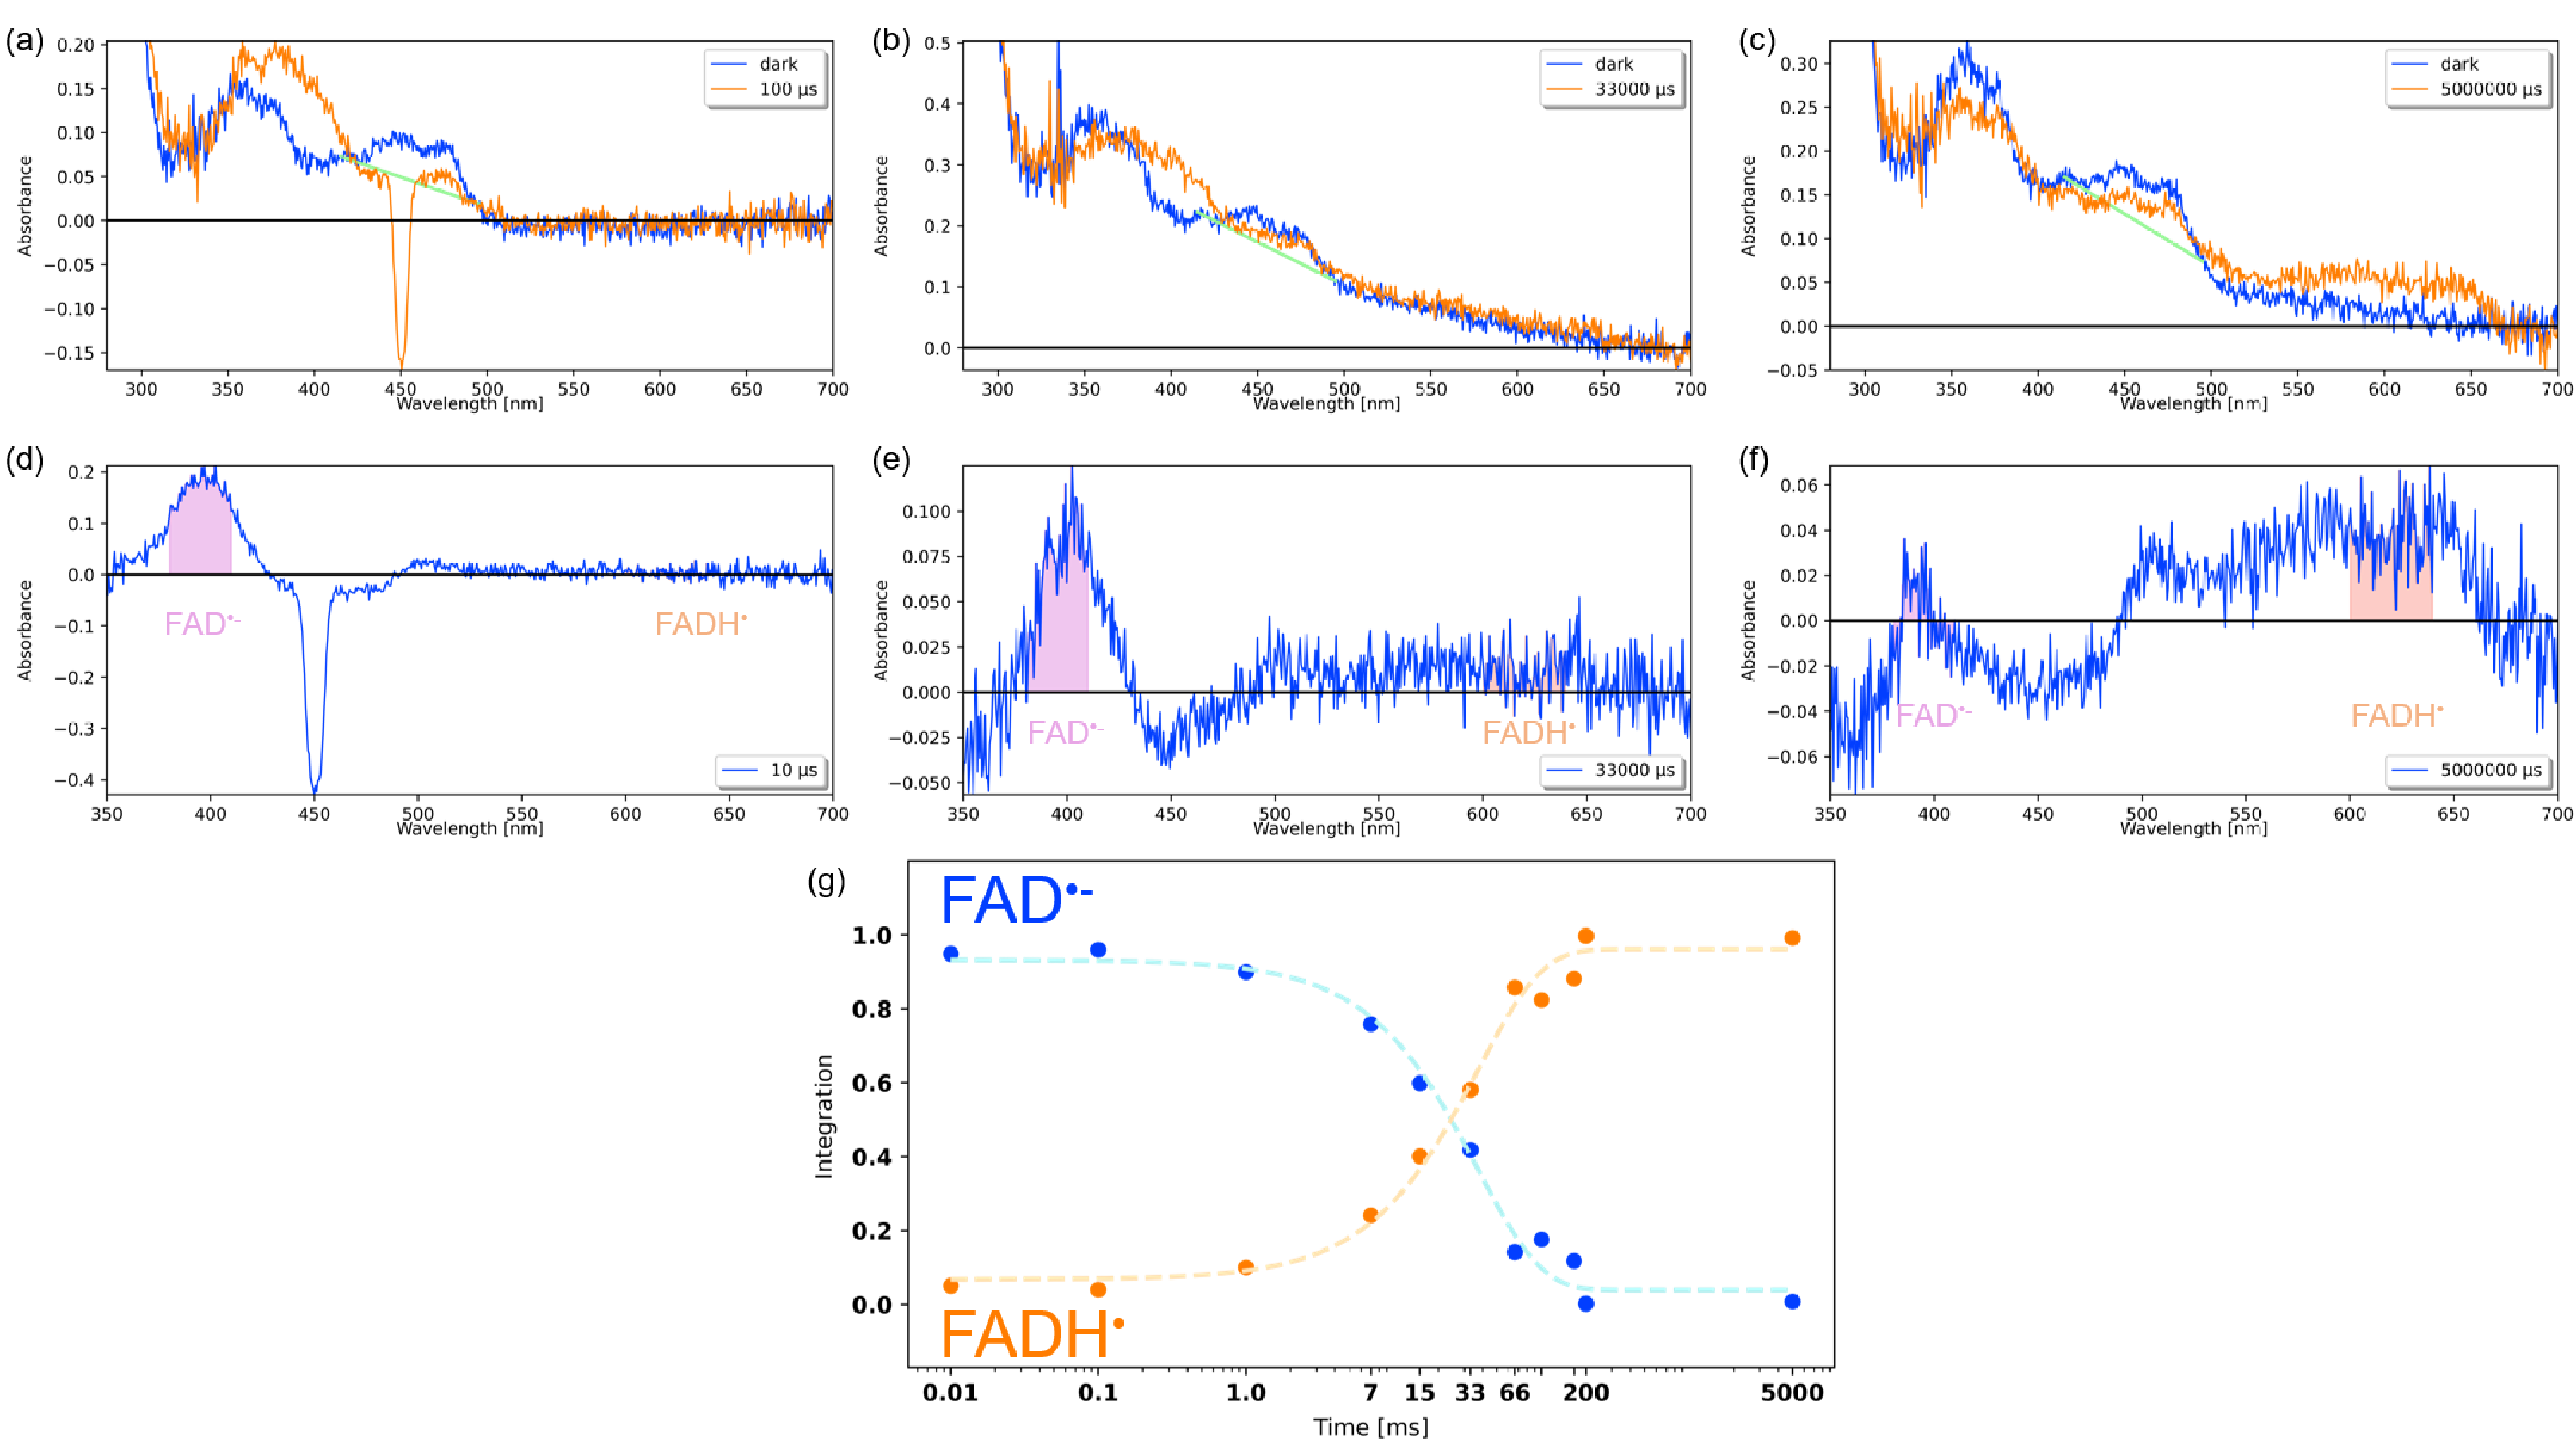
\includegraphics[width=\textwidth]{images/cracry/TRicOS_cracry.pdf}
  \hfill
  \caption{Time-resolved \textit{in crystallo} UV-vis absorbance spectra analysis. (a) (b) and (c): time-point (orange) and corresponding dark (blue) spectra at 100 \textmu s, 33 ms and 5 s, respectively. The peak corresponding to the anionic semiquinone FAD\textsuperscript{•-} around 300 nm is visible at 100 \textmu s (a). The peak corresponding to the neutral semiquinone FADH\textsuperscript{•} is also visible between 550 nm and 650 nm at 5 s (c). (d), (e) and (f): \(AS_{time point}-AS_{dark}\) difference spectra for time points 100 \textmu s, 33 ms and 5 s, respectively. The area integrated to assess the anionic semiquinone FAD\textsuperscript{•-} is coloured in pink, while the area integrated to assess the neutral semiquinone FADH\textsuperscript{•} is coloured in salmon. (g) Integrated, normalised absorbance over time in logarithmic scale for FAD\textsuperscript{•-} (blue) and FADH\textsuperscript{•} (orange) represented as dots, with corresponding mono-exponential reaction curves (dashed). The time constant of the modelled curve is 37 ms.}\label{fig:TRicOS_CraCRY}
\end{figure}

The laser pulse energy was adjusted to three different light fluences at sample position (95 mJ/cm\textsuperscript{2}, 295 mJ/cm\textsuperscript{2} and 482 mJ/cm\textsuperscript{2}) to inspect whether artefacts related to multiphoton absorption occurred. For each of these three energy levels, the time-constant obtained was virtually identical, respectively of 36 and 37 ms and 37 ms.

\section{Protonation mechanism elucidated thanks to TR-\textit{ic}OS}

With the protonation window having been assigned to the 10-100 ms region of the time-course, the slight changes within the first three microseconds (Fig. \ref{fig:CraCRY_protonation} (b)) can be assigned to the relaxation of the isoalloxazine’s geometry after electron transfer. Before the flavin cofactor returns to a conformation comparable to that which it adopts in steady-dark, oxidised structure, compensatory movements of the highly conserved R360-D389 salt bridge packing against the FAD\textsuperscript{•-} isoalloxazine ring group occur. This explains their movements during the \textmu s region of the time course, despite them not being the proton donor. 

Knowing that the protonation occurs in the early ms regime, we assigned the evolution difference electron density observed on N395 patterns to its interaction with either FAD\textsuperscript{•-} or FADH\textsuperscript{•} radicals. Between 10 ns and 33 ms, a clockwise rotation relative to the dark, oxidised state (\textDelta chi2: -86.4\degree) positions the N395 sidechain within hydrogen bonding distance between its N\textdelta 2 atom and the FAD\textsuperscript{•-} N5 nitrogen (Fig. \ref{fig:CraCRY_protonation} (b)). Between 66 ms and 233 ms, a counter-clockwise rotation almost restores the dark, oxidised state conformation (\textDelta chi2: +111\degree) of this N395/FAD switch by forming now a hydrogen bond between the protonated N5 nitrogen of FADH\textsuperscript{•} and the N395 O\textdelta 1 atom. 

\section{Unravelling the C-terminal events with local SVD analysis}\label{sec:SVD_CraCRY}

The flip of the D321 side-chain is visible as early as 10 ns after the pump of the 450 nm laser and is conserved all through the TR-SFX series (Fig. \ref{fig:CraCRY_Cter}). It is even the strongest feature in all of the maps, which demonstrates the unique role of D321 as the proton acceptor in the last PCET step of the electron transfer chain (Fig. \ref{fig:CraCRY_photoreaction} (a), \cite{lacombatUltrafastOxidationTyrosine2019}).

As visible in Fig. \ref{fig:CraCRY_photoreaction} (b), \textalpha22 interacts in the FADox state with the PHr domain via hydrophobic contacts and salt-bridges, particularly two 'anchors': D321-R492 and D323-R485 (Fig. \ref{fig:CraCRY_Cter}). The change protonation of D321 after PCET results in a light-triggered strain within the D321-R492 anchor point of \textalpha22 (Fig. \ref{fig:CraCRY_Cter} (a)). The second anchor point is affected early in the \textmu s (Fig. \ref{fig:CraCRY_Cter} (b)), which ends up disordering the tip (residues R494 to R485) of helix \textalpha22 on a millisecond time scale (Fig. \ref{fig:CraCRY_Cter} (c)). Inexplicably though, the disorder does not progress much further along the helix, and the intensity of negative peaks in the isomorphous \(F_{obs}(200 ms) - F_{obs}(dark)\) electron density map has decreased, compared to the peaks visible at 1 ms (Fig. \ref{fig:CraCRY_Cter} (d)). This is unlikely to be the consequence of a radical quenching of Y373\textsuperscript{•} allowing the C-ter to re-fold, as the FADH\textsuperscript{•} absorption band remains 5 s after the actinic light pulse. 
\begin{figure}[H]
  \centering
  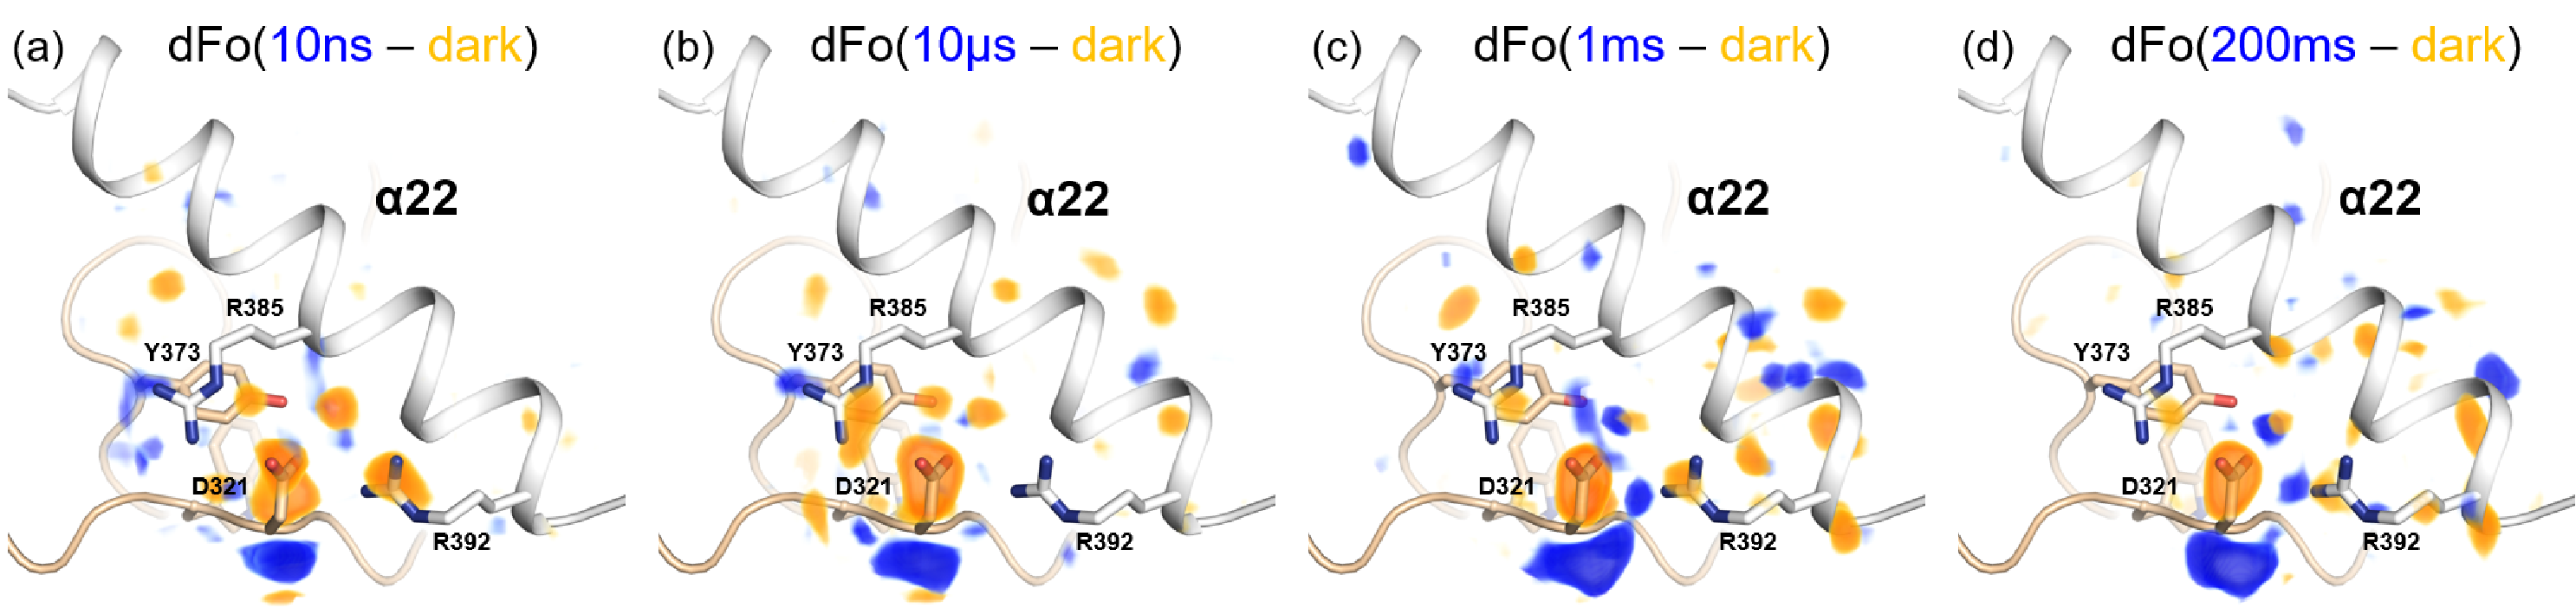
\includegraphics[width=\textwidth]{images/cracry/CraCRY_C-ter.pdf}
  \hfill
  \caption{Isomorphous \(F_{obs}(time\ point) - F_{obs}(dark)\) electron density maps features around the \textalpha22 (white), and its anchor points to the PHr domain (wheat) D321, contoured at 3.5 \textsigma level and overlaid on the oxidised state model (negative electron density is coloured gold, while positive electron density is coloured blue). (a) 10 ns after the pump laser pulse, a strong negative peak on D321, coupled with a strong positive peak under the backbone of its strand, indicates that it has flipped. Correspondingly, a negative peak on R392 indicates that it is head is displaced. Both these movements rupture one of the anchor points of \textalpha22. (b) 10 \textmu s after the pulse, the pair of peaks of D321 have increased in intensity, and peaks on each side of R385 show that it is now shifting too. Specks of negative peaks can be seen around the backbone of \textalpha22. (c) After 1 ms, a pair of peaks indicates that D321/R394 and D323/R385 are both shifting apart, and both anchor points are ruptured. The negative electron density around the backbone of \textalpha22 is slightly stronger and can be seen up to C482. (d) 200 ms after the pulse, the negative electron density peak on R485 has decreased, and so has the signal around the backbone of \textalpha22.}\label{fig:CraCRY_Cter}
\end{figure}
The dynamics of the C-terminus are complex, with two apparent components: an initial disordering and a later reordering of the \textalpha22 helix. They are also subtle, as the difference electron density peaks on \textalpha22 are much weaker than those caused by the flip of the nearby D321 side chain. Further, the disorder of \textalpha22 sets in long after the flip of D321. 
\vspace{2mm}

We leveraged an improved SVD analysis to deconvolute the dynamics of the C-terminus to clarify the sequence of events. 

\subsection{Improvements to the SVD analysis pipeline}

Attempts at full-maps or local SVD analyses produced lSV time-invariant structural components dominated by the movements of D321, Y373 and other amino acids of the PHr domains. To focus the analysis on \textalpha22, the maps used as inputs to the analysis were masked around the helix: electron density values in all voxels further than 1.8 \AA\ away from \textalpha22 were set to 0. This was accomplished using the \textit{mask-map-by-molecule} function of Coot \parencite{emsleyFeaturesDevelopmentCoot2010}.

The isomorphous difference electron density maps are calculated identically as in Section \ref{sec:SVD_Methods}, however, the resulting difference structure factors (in the mtz format) are loaded directly into Python using the GEMMI python package \parencite{yamashitaGEMMIServalcatRestrain2023}. From these structure factors, a real-space difference electron density map can be calculated with the desired sampling rate using the FFT implementation of the GEMMI package. With this improvement, we no longer need to cut all maps at the same resolution. The rest of the procedure is similar to what is described in Section \ref{sec:SVD_Methods}.

Once the electron density values of a map are stored in a numpy array (thanks to GEMMI), and given that we know the sampling rate of the map, we can calculate the electron density in a given volume (this is referred to as density integration). Density integration is routinely used for the analysis of TR-MX data, to identify the trends in a series of electron density maps \parencite{wickstrandToolVisualizingProtein2020, maestre-reynaVisualizingDNARepair2023a}. Re-convoluted maps can be obtained using the equation presented in Section \ref{sec:SVD_MmCPDII}, but limiting the sum to the number of components deemed meaningful in the analysis. Then, the integrated electron density in the region of interest can be plotted against time, along with the integrated electron density from the experimental maps. This plot constitutes a simple validation procedure to confirm that the dynamics of the system - here, the unfolding/refolding dynamics - are effectively captured by the components the user has chosen, taking away some of the subjectivity in SVD analysis \footnote{The original idea of integrating re-composed maps after SVD analysis comes from Yuhei Hosokawa and Manuel Maestre-Reyna, but was intended as a way to estimate the occupancy of each of the reaction states singled out by the analysis, to guide structure factor extrapolation.}. 

\subsection{Incomplete unravelling of the C-terminus}

The meaningful lSVs are presented in Fig. \ref{fig:CraCRY_Cter-SVD} (a) and (b). Their time-varying rSVs (their magnitude, which is the product of their amplitude and their polarity, over time) are plotted in Fig. \ref{fig:CraCRY_Cter-SVD} (c).  The integrated negative density for input and reconstructed maps are plotted against time in Fig. \ref{fig:CraCRY_Cter-SVD} (d).

Integrating negative difference electron density around \textalpha22 reveals that after an initial disordering phase from 1 to 100 \textmu s, the negative difference electron density around the C-terminus decreases in intensity, to reach an intermediate phase whose intensity is one-third of that of the most disordered state (black curve, Fig. \ref{fig:CraCRY_Cter-SVD} (d)). We used singular value decomposition (SVD) of difference electron density maps restricted to the volume of \textalpha22 to elucidate the reason for the apparent re-ordering of \textalpha22. 

Using the density integration validation procedure proposed above, we can validate that lSV0 and lSV1 are sufficient to explain the dynamics of \textalpha22 (Fig. \ref{fig:CraCRY_Cter-SVD} (d)), as the evolution of the integrated density of the experimental maps and re-convoluted maps follow the same trend.  We propose that lSV0 and lSV1 explain the dynamics of \textalpha22 during the late stages of CraCRY photoreduction: the main time-invariant structural component, lSV0, is characterized by an accumulation of negative difference electron density around the C-terminal half of \textalpha22 end (Fig. \ref{fig:CraCRY_Cter} (a)), we therefore suggest that it represents the disordering of \textalpha22. lSV0 also comprises the negative electron disordering of R492 and the conformational change of R485. Its magnitude, rSV0, dominates the time course from 1 \textmu s on, (black curve in Fig. \ref{fig:CraCRY_Cter} (c)), gradually increasing in amplitude until 100 \textmu s. Interestingly though, rSV0 decreases steadily after 1 ms. 

lSV1 features pairs (positive and negative) of difference electron density peaks on the entire length of \textalpha22 (Fig. \ref{fig:CraCRY_Cter} (c)). The negative peaks are located at the interface between \textalpha22 and the PHr domain, while the corresponding positive peaks are on the solvent side of the helix. Importantly, the peaks contained in lSV1 are uniformly dispersed along \textalpha22, and not only at its tip or its farthest half. This component can be interpreted as a uniform sliding movement, away from the PHr domain and into the solvent. Finally, a positive peak on R492 indicates that this slide movement comes with the restoration of the first anchor points of \textalpha22.  From 10 ns to 30 \textmu s, rSV1 is negative, and slowly decreases in amplitude (red curve in Fig. \ref{fig:CraCRY_Cter} (c)). As a consequence, the multiple positive peaks of the reversed-polarity lSV1 (Fig. \ref{fig:CraCRY_Cter} (c)) decrease in intensity, which ends up contributing to the overall rise of negative electron density on \textalpha22. From 100 \textmu s on, though, rSV1 is positive, and its amplitude increases marginally. Combined with the decay of the amplitude of rSV0, this causes the emergence of a new, shifted but stable, conformation of \textalpha22, partially replacing the disordered helix. 

Since SV1 magnitudes contribute positively in the later stages of our time course (Fig. \ref{fig:CraCRY_Cter}h), we believe it is reasonable to describe it as a long-lived intermediate in a competing reordering process, in opposition to further disordering promoted by SV0.
\begin{figure}[H]
  \centering
  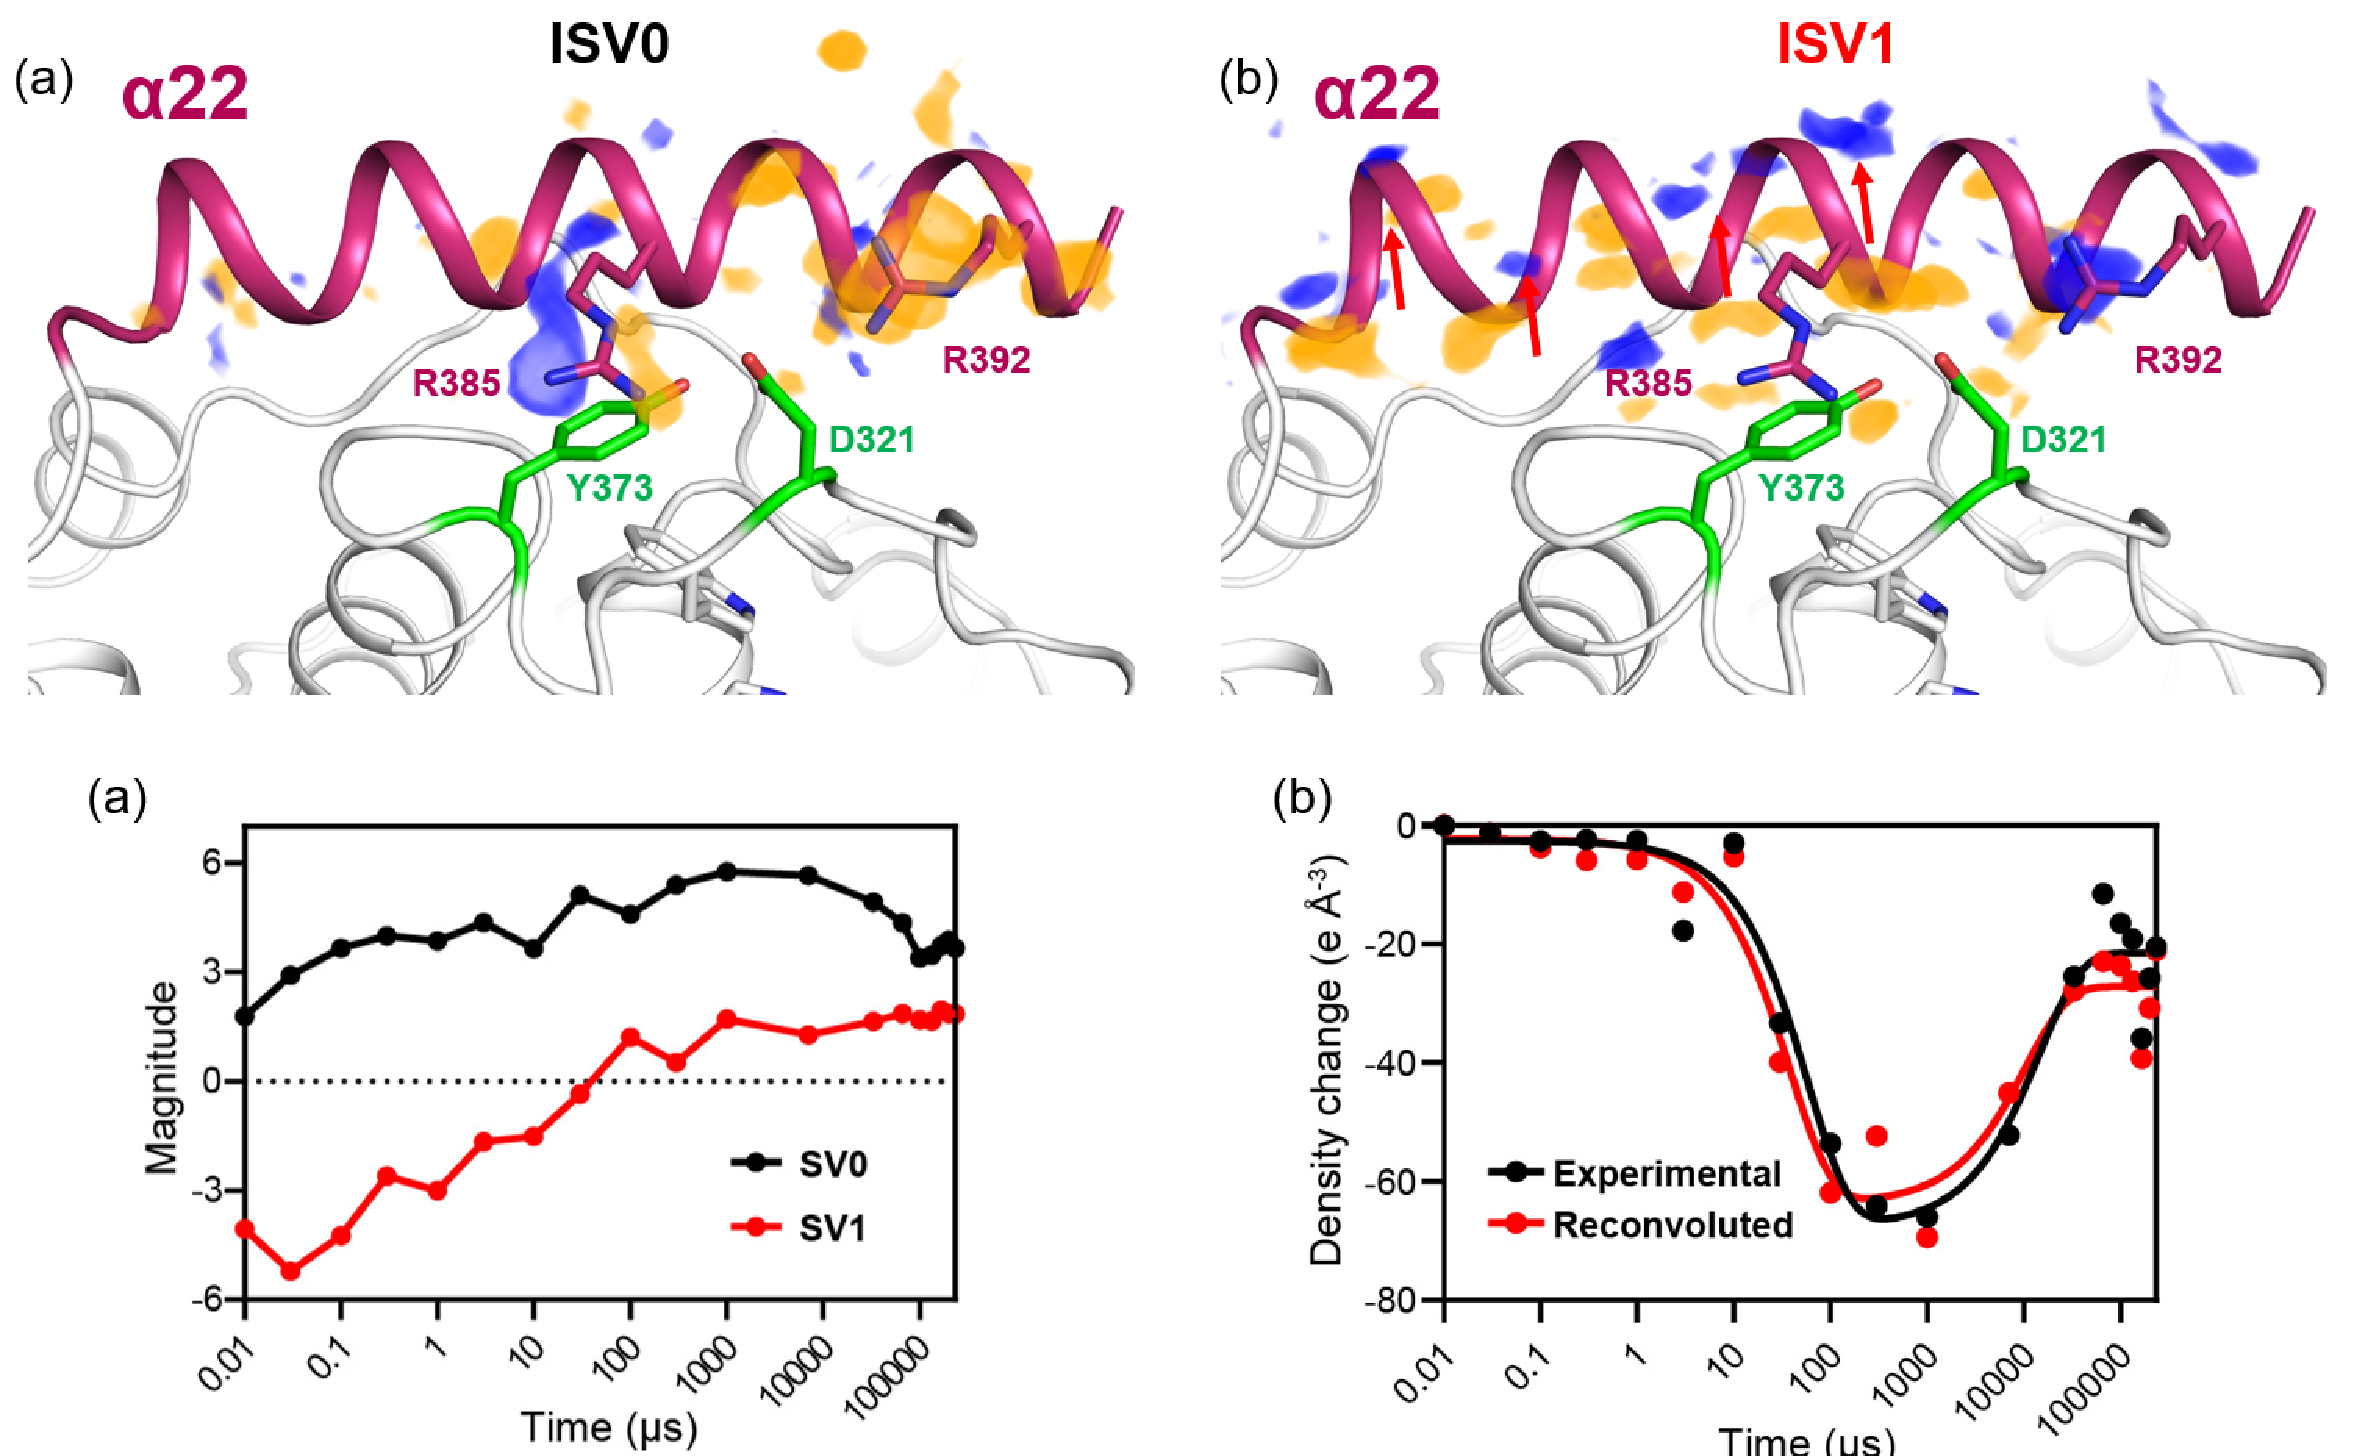
\includegraphics[width=\textwidth]{images/cracry/CraCRY_C-terSVD.pdf}
  \hfill
  \caption{Local SVD analysis of the dynamics of \textalpha22 (a) and (b): main time-invariant structural component lSV0 and lSV1, overlaid over \textalpha 22 (purple), with its main switch (Y373/D321, coloured in green) and two anchor points to the PHr domain (white). (a) lSV0 features negative difference electron density all over the backbone of the tip of \textalpha22 (residues 485 to 494) and negative peaks on selected residues up to C482. R492 is entirely covered by negative electron density, indicating its disorder, while a strong pair of peaks indicates the shift of R485 away from the cluster of interaction anchoring \textalpha22. (b) lSV1 features a series of negative peaks on the entire surface of interaction with the PHr domain and  \textalpha22, coupled with a series of positive peaks on the solvent side of the helix. This suggests that lSV1 represents a sliding movement, PHr domain. (c) Time-dependent traces of rSV0 (black) and rSV1 (red) plotted over time. The amplitude of rSV0 gradually increases in the early time points but decays later. Meanwhile, the polarity of rSV1 is initially negative and switches after \textasciitilde30 \textmu s. (d) Time-dependent negative difference electron density evolution around \textalpha22 (black dots) fits a two-step kinetics model (continuous black line). The difference electron density integrated in the map re-convoluted with the two main SVD components (red) and follows the same kinetics (continuous line) as the density integrated in the experimental maps (red). }\label{fig:CraCRY_Cter-SVD}
\end{figure}
In summary, SVD analysis reveals that \textalpha22 disordering is slow, and without intermediates. This \textalpha22 transition corresponds closely to other strain-driven protein quakes \parencite{ansariProteinStatesProteinquakes1985} as initially defined by the ultrafast myoglobin-CO system and found later for the PYP \parencite{xieFormationNewBuried2001,renMolecularMovieResolution2001a}.  Meanwhile, the competing reordering process, which occurs during the later stages of our time course, follows more traditional protein-folding kinetics with a structural intermediate described by SV1. It produces the 'slid-away' conformation of \textalpha22, which is slightly dissociated from the PHr region. 

A recent characterisation of light-triggered conformational changes in CraCRY by time-resolved ion-mobility mass spectrometry identified the complete dissociation of \textalpha22 from the PHr domain as the main consequence of the illumination by a 450 nm LED \parencite{zanglTimeResolvedIonMobility2024}. A second significant finding of this article is that the dissociation of \textalpha22 from the PHr domain is reverted after the illumination ends, with a rate constant of \textasciitilde0.2 s, which is in the same order of magnitude as the time-points during which the refolding starts to happen (>33 ms). The existence of the refolded 'shifted' conformation of \textalpha22 represented by lSV1 can be explained as a refolding event. However, only the tip of \textalpha22 is disordered in the conformation represented by lSV0 (Fig. \ref{fig:CraCRY_Cter-SVD}) while the helix is fully dissociated from the PHr domain in \cite{zanglTimeResolvedIonMobility2024}. Therefore, since the state achieved in the last time-point of the series (233 ms) does not match the 'dissociated' \textalpha22 state characterised in \cite{zanglTimeResolvedIonMobility2024}, it is unclear whether the signalling state has been achieved in this series. The packed environment of the crystal may inhibit the unfolding of \textalpha22. 

\section{Conclusion}

Here, the use of TR-\textit{ic}OS as a complement to TR-SFX data was indispensable to guide the interpretation of the features present in the isomorphous \(F_{obs}(time\ point) - F_{obs}(dark)\) electron density map. Knowledge of the respective FAD\textsuperscript{•-} and FADH\textsuperscript{•} occupancies over time allowed us to identify the residues involved in a protonation pathway from the solvent to the flavin cofactor and adequately model the reaction intermediates involved in the stabilisation of the radical semiquinone flavin in its anionic and then protonated form. Additionally, an improved SVD analysis allowed us to fully elucidate the dynamics governing the disorder of the C-terminus in the series. These complementary spectroscopic and extensive crystallographic analyses were needed to optimally exploit the rich TR-SFX data. The structural interpretation of all the structural events in the rest of the protein over the series was achieved by the team of Manuel Maestre at the National Taiwan University (NTU), and will not be described here. 
\vspace{2mm}
Yet, at the end of the series - that is to say, 233 ms after the actinic light pulse - the doubt remains as to whether we have observed the putative signalling state identified in \cite{zanglTimeResolvedIonMobility2024}. This doubt begs the question: what happens at longer delays after the photoreduction of the flavin cofactor?
\vspace{2mm}
In an attempt to catch the putative signalling state in which \textalpha22 is dissociated from the PHr domain, longer delays after illumination were sampled via pump-probe TR-SFX and TR-SSX. Unfortunately, the viscous medium extruder used at SACLA and on beamlines Alvra at SwissFEL and PXI at the SLS is not well suited to measuring time points past 300 ms after the pump optical laser pulse. Past this limit, the displacement of the viscous medium between the pump and probe pulses cannot be neglected anymore: the interaction point of the optical laser and that of the X-ray beam have to be offset. Because the speed of the viscous medium is not perfectly constant, it is difficult to guarantee that the crystals illuminated by the pump are indeed the ones getting exposed to the X-ray beam after the set delay. This makes the occupancy of the activated state unstable from time-point to time-point, greatly complicating the interpretation of the data. Fixed target or tape drive setups such as the one used in Part \ref{part:T-Cer} are more suited to this kind of experiment. 
\vspace{2mm}
Crucially, Zangl and collaborators utilised continuous illumination for their time-resolved ion-mobility mass spectrometry study \parencite{zanglTimeResolvedIonMobility2024}. It is therefore also possible that more than one activation event is necessary to produce the putative signalling state where \textalpha22 is dissociated from the PHr. 
\vspace{2mm}
We leveraged an improved version of the original TR-SOX method (described in Section \ref{sec:LOV2_TR-SOX}), combining continuous illumination and sampling the ms to s time-domain to explore the transition from the initial disruption of the main anchor of \textalpha22 (the D321-R492 salt bridge) to the putative signalling state. 


\chapter{Visualising the build-up of the signalling state of a cryptochrome with the TR-SOX method}\label{chap:CraCRY_TR-SOX}

\section{A steady-light recorded on CraCRY crystals under continuous illumination}

\subsection{The diffracting power of CraCRY crystals is maintained during continuous illumination but lost with a pump-probe scheme}
During the pump-probe, long delay TR-SX experiments mentioned above, it was noted that the diffracting power of the crystal greatly decreased after illumination as time went on (past 300 ms). Conversely, we found that the diffracting power of larger (\(300 \times 50 \times 40\) \textmu m\textsuperscript{3}) oxidised CraCRY crystals, preserved at room temperature with a humidity-controlling device \parencite{sanchez-weatherbyImprovingDiffractionHumidity2009} was comparable when they were mounted under safety red lights without actinic illumination (2.2 \AA\ resolution limit) and after a 14 min illumination with a continuous wave (CW) 440 nm laser (2.4 \AA\ resolution limit). This experiment took place at beamline ID30A3, ESRF \parencite{vonstettenID30A3MASSIF3Beamline2020}, where the laser was mounted to illuminate the sample position with a 720 \textmu m radius focal spot (5 mW) (Fig \ref{fig:TR-SOX_exp} (b)). Importantly, no reducing agent was soaked in the crystal illuminated for 15 minutes, meaning that it stalled in the FADH\textsuperscript{•} state and could not transition to the fully reduced FADH\textsuperscript{-} state\parencite{lacombatUltrafastOxidationTyrosine2019}.

Strikingly, the lattice parameters of CraCRY are affected by the illumination, most notably its C-axis, which shrinks by \textasciitilde6 \AA\ (Table \ref{tab: UC_CraCRY_steady}). A possible reason why the diffraction power of the crystals is better conserved with the continuous illumination setup deployed on ID30A3 while it was lost during the pump-probe experiment is that, during the pump-probe experiment, only a fraction of the crystals get activated. In these conditions, part of the crystal lattice transforms to reach a 'steady-light lattice' while the rest remains in the 'steady-dark lattice' state, destroying the overall crystalline order of the crystal. 
\begin{table}
    \centering
    \begin{tabular}{ccccccccc}
         Dataset&   Resolution (\AA)& Symmetry&a&  b&  c&  \textalpha&  \textbeta& \textgamma\\
         dark&   2.2& P 2\textsubscript{1} 2\textsubscript{1} 2\textsubscript{1}&51.2&  66.0&  155.8&  90&  90& 90\\
         steady-light&   2.4& P 2\textsubscript{1} 2\textsubscript{1} 2\textsubscript{1}&50.9&  65.4&  150.0&  90&  90& 90\\
    \end{tabular}
    \caption{Diffraction resolution, symmetry, and lattice parameters of a crystal mounted under red safety lights before (steady-dark) and after (steady-light) illumination. CraCRY MX structures, collected at room temperature.}
    \label{tab: UC_CraCRY_steady}
\end{table}

\subsection{Comparing steady-dark and steady-light structures with a real-space difference map}

In steady-dark structure of CraCRY recorded on ID30A3 (will be referred to as steady-dark), \textalpha22 is stable, and folded exactly in the same conformation as in our dark, oxidised structure recorded at SACLA (Chapter \ref{chap:CraCRY_TR-SFX_1} )\footnote{The FAD cofactor of cryptochrome and photolyases is susceptible to specific radiation damage. This has been utilised in the past to initiate the DNA repair mechanism \parencite{meesCrystalStructurePhotolyase2004}. While the resolution of the synchrotron dark structure does not permit us to fully observe the reduction of the FAD cofactor by the X-ray beam, it cannot be ruled out. Nevertheless, this does not seem to affect the C-terminal helix, which is intact in the SSX structure.}.  Comparing this structure with the steady-illuminated might produce valuable insight on exactly which regions of the proteins are exposed to the solvent after \textalpha22 dissociates from the PHr domain and are therefore free to interact with protein partners to further relay their signal to a cell. 
\vspace{2mm}
The large difference in the c-axis value between steady-dark and steady-light prevents the use of an isomorphous difference \(F_{obs}(steady\mbox{-}state) - F_{obs}(dark)\) electron density map. Thus, steady-dark and steady illuminated structures were first analysed via a \(steady\mbox{-}state - dark\) real-space electron density difference map, obtained using a newly published methodology \parencite{brooknerMatchMapsNonisomorphousDifference2024}. 
\vspace{2mm}
All of the difference electron density peaks of this map are concentrated in the region of \textalpha22 and, the strands stabilising it (Fig. \ref{fig:TR-SOX_ligh_dark_steady_CraCRY} (a)). Negative difference electron density all over \textalpha22 indicates that it is fully unfolded, while a strong positive peak above the helix indicates that the disordered hinge region is now pointing away from the PHr domain. Close by, a series of positive peaks on the left side of the loop formed by residues 415 to 420 indicates that it has shifted away from \textalpha22. A series of positive peaks over the strand carrying Y373 indicate that the entire strand has switched conformation in the illuminated structure, and is not simply disordered. Strikingly, the main feature of the TR-SFX series, the pair of peaks around D321 (Fig. \ref{fig:CraCRY_Cter}), are not visible in the map, Instead, most strands interacting with \textalpha22 seem fully disordered. 

The negative difference electron density on the strands of the PHr domain are much stronger than those on \textalpha22, possibly because the PHr domain is already much more stable in steady-dark, and therefore, its disordering creates a larger change than the disordering of \textalpha22, which sits at the edge of the protein. 

The atomic model of steady-light (coloured blue) structures differs the most from the model of steady-dark (coloured beige) in the region of \textalpha22 (Fig. \ref{fig:TR-SOX_ligh_dark_steady_CraCRY} (b)). In steady-light, \textalpha22 is fully disordered, in perfect accordance with the state described in \cite{zanglTimeResolvedIonMobility2024}. Additionally, two regions nearby, N314-D324 (which includes D321 and Y373) in the α13/α14 loop as well as A404-Q410  in the α18/α19 loop (background of the panel (b)), are disordered in steady-light (Fig. \ref{fig:TR-SOX_ligh_dark_steady_CraCRY} (b)). Conversely, the loop carrying Y373 shifts 'up' to into the space previously occupied by \textalpha22. With W322 and D321 released from their tight interaction with Y373, the electron transfer chain described in Fig. \ref{fig:CraCRY_photoreaction} (b) is severed in steady-light. 
\vspace{2mm}
This finding is quite significant: when the putative signalling state (represented by steady-light) is achieved, further photoreduction of the flavin cofactor into the fully reduced FADH\textsuperscript{-} state, i.e. CraCRY’s catalytically competent form as photolyase is impossible. This suggests that CraCRY will go down the photolyase route if a partner is capable of reducing Y373\textsuperscript{•} back into a neutral state before the large-scale disordering of the \textalpha22 occurs, and will otherwise go down the 'signalling route', which forbids electron transfer for the entire lifetime of the signalling state. 
\vspace{2mm}

Strikingly though, effects around the flavin cofactor are extremely moderate (Fig. \ref{supfig:TR-SOX_qFo_FAD} ), in opposition with the ample movements observed upon photoreduction and DNA repair of a Class II photolyase \parencite{maestre-reynaSerialCrystallographyCaptures2022, maestre-reynaVisualizingDNARepair2023a}. This is easily explained however, as animal-like cryptochromes (such as CraCRY) evolved from 6-4 photolyases \parencite{meiEvolutionaryHistoryPhotolyase2015}, and recent structural studies of a 6-4 photolyase display a consistent lack of angular perturbation of the FAD upon photoreduction \parencite{celliniStructuralBasisRadical2022, celliniDirectedUltrafastConformational2024}. Most notably, N395 is in the same position in steady-light and steady-dark (Fig. \ref{supfig:TR-SOX_qFo_FAD} (f)), which indicates that the change of conformation observed during photoreduction and protonation of the flavin cofactor (Fig. \ref{fig:CraCRY_protonation}) is only a mean of transient stabilisation. 
The large-scale disordering of \textalpha22 and its support strand (N314-D324) is likely the cause of the changed lattice parameters for the illuminated state (Table \ref{tab: UC_CraCRY_steady}). 
\begin{figure}[H]
  \centering
  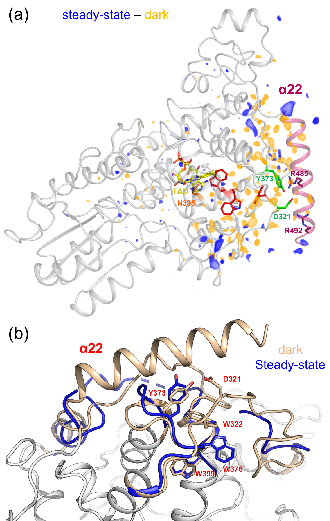
\includegraphics[width=0.8\textwidth]{images/cracry/light-dark_MX.pdf}
  \hfill
  \caption{Comparing steady-dark and steady (15 min) illuminated synchrotron room-temperature structures of CraCRY. (a) Real-space electron density \(steady\mbox{-}state - dark\) computed with \cite{brooknerMatchMapsNonisomorphousDifference2024}. Negative peaks are shown in gold, positive peaks in blue, and the signal is contoured at 3.5 \textsigma level Very strong negative electron density covers the strands involved in the support of \textalpha22 and the helix itself. The signal in this map is concentrated on the 'southeast' section of the protein.  The strand carrying D321 and W222 is entirely covered in negative difference electron density. Positive peaks near residues 415: 420 indicate that their strand has shifted away from \textalpha22. Positive peaks near Y373 indicate that its strand has switched conformation. (b) refined models corresponding to steady-dark (wheat, residues unaffected by the illumination are coloured in white) and illuminated steady-light structures (blue). The entire \textalpha22 helix is disordered. The loop carrying Y373 has shifted down, allowing Y373 to twist and shift into the space previously occupied by \textalpha22. The strand carrying D321 and W322 is entirely disordered.}\label{fig:TR-SOX_ligh_dark_steady_CraCRY}
\end{figure}

Since continuous illumination does not seem to affect the diffraction power of crystals of 100s of \textmu m, we investigated the late stages of the transition from ground to signalling state of CraCRY via the TR-SOX method \parencite{aumonierMillisecondTimeresolvedSerial2020}. 

\section{Appraising the transition to a steady-state with a TR-SOX series}

\subsection{Improvements made to the TR-SOX technique}
Briefly, with the TR-SOX method (described in Section \ref{sec:LOV2_TR-SOX}), large (\(> 100\) \textmu m\textsuperscript{3} crystals are mounted on the axis of the goniometer of a standard MX beamline (here, ID30A3-MASSIF3 at the ESRF, sample environment is visible in Fig \ref{fig:TR-SOX_exp} (b)) and maintained at 97 \% humidity, at room temperature using a humidity controller \parencite{sanchez-weatherbyImprovingDiffractionHumidity2009}. An oscillation data collection starts synchronously with a continuous actinic illumination. The process is repeated for tens to hundreds of crystals. These datasets are then chopped into wedges, which form time-points linearly dispersed along the data-collection time. 
\subsection{Data collection scheme}
In original study of the LOV2 domain of the Phototropin II of \textit{Arabidopsis thaliana} via the TR-SOX technique \parencite{aumonierMillisecondTimeresolvedSerial2020}, isomorphous difference \(F_{obs}(time\ point) - F_{obs}(dark)\) maps could not be calculated, presumably because of a lack of isomorphism. In an attempt to remediate that issue, the procedure was altered to delay the start of the actinic illumination compared to the start of data collection (Fig \ref{fig:TR-SOX_exp} (a)). As a result, the first wedges of each crystal can be merged to produce a dark dataset (dark-SOX), which should be more isomorphous to the rest of the time-point than an MX structure would be. To create the delay, the TTL signal sent to the X-ray detector by the timing module of the micro diffractometer of the beamline was replicated, after a set delay, and passed on to the actinic laser (Fig \ref{fig:TR-SOX_exp} (c)). 
\vspace{2mm}
In solution, under blue light illumination, the '\textalpha22 dissociated' putative signalling state is achieved with a rate constant of 0.12 s in \cite{zanglTimeResolvedIonMobility2024}. \textit{In crystallo}, large domain rearrangement can often be delayed because of the crystalline packing induced rigidity, decreased hydration or the viscosity of crystallisation conditions (compared kinetics in solution and \textit{in crystallo} are discussed in more detail in Chapter \ref{chap:toolbox}.). Therefore, we chose to explore a relatively long delay after the start of illumination (5.8 s) to have a chance to observe the true signalling state. 

For each crystal, a dataset of 600 images corresponding to a full rotation of  180 \degree\  \footnote{twice the minimal range needed for a full dataset of a crystal in space-group P 2\textsubscript{1} 2\textsubscript{1} 2\textsubscript{1}} and a duration of 6 s was collected (Fig. \ref{fig:TR-SOX_exp} (a)). These datasets were chopped into 30 wedges of 20 images (200 ms). Accordingly, we then set a delay of 200 ms between the beginning of data collection and illumination, resulting of 20 images for the dark-SOX wedge. This process was repeated on 88 crystals of CraCRY, resulting in dark-SOX, and 29 \(n\)-SOX datasets, each separated by 200 ms, spanning from 200 ms to 5.8 s after the start of the illumination.
\begin{figure}[H]
  \centering
  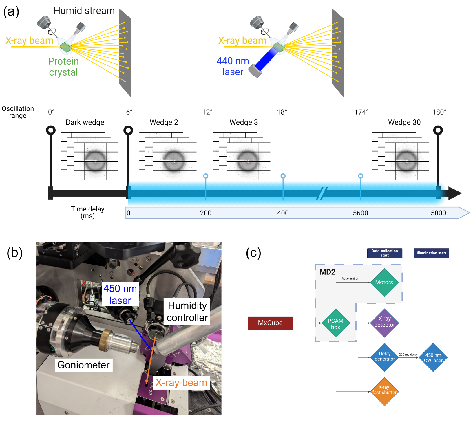
\includegraphics[width=\textwidth]{images/cracry/TR-SOX_exp.pdf}
  \hfill
  \caption{The TR-SOX experimental scheme. (a) Crystals of CraCRY are manually mounted and centred at room temperature, on beamline ID30A3-MASSIF3, at the ESRF. Their humidity is maintained by a humidity controller \parencite{sanchez-weatherbyImprovingDiffractionHumidity2009}. A standard MX data-collection is started, with 0.3 \degree of oscillation range, 10 ms of exposure and a total rotation of 180 \degree (6 s). After 200 ms, a 450 nm, continuous wave laser is turned on. The 6s dataset is chopped into wedges of 200 ms (6 \degree, 20 images), with the first wedge being the resting state. This process is repeated several times over, and wedges corresponding to the same time scale are processed together. (b) On beamline ID30A3, the micro diffractometer (MD2) synchronizes the data collection elements through its timing module (PCAM box). Upon receiving the signal from MxCube, the MD2 primes its motor and accelerates to reach the desired rotation speed. Then, when data collection starts, a TTL signal is sent to the fast shutter, the X-ray detector and to an electronic delay generator so that the signal would only reach the continuous wave laser 200 ms
after the beginning of data collection, allowing part of the dataset to correspond to the dark state.}\label{fig:TR-SOX_exp}
\end{figure}
\subsubsection{Data-processing}

The data-processing procedure was significantly altered from that of \cite{aumonierMillisecondTimeresolvedSerial2020}, in favour of a custom analysis pipeline, branching from KAMO \parencite{yamashitaKAMOAutomatedData2018} (Fig. \ref{fig:TR-SOX_proc}). We chose not to use the full KAMO package because it performs a series of tests inside each wedge, in particular, removing the images exhibiting particularly mosaic spots.  As the reaction progresses in the crystal, mosaicity inevitably increases, meaning that KAMO would remove precisely the images containing the most information for a TR-MX experiment. 

Each wedge in a pack was indexed and integrated with XDS \parencite{kabschXDS2010} with no prior knowledge. Then its space group was determined by pointless \parencite{evansIntroductionDataReduction2011} \footnote{It was empirically found that the space group determined by pointless was more likely to be the correct P 2\textsubscript{1} 2\textsubscript{1} 2\textsubscript{1} than that found by XDS.}. At that point, the most abundant space group (consensus) was chosen. The lattice parameters of all datasets indexed in the same point group as the consensus were averaged. This provided prior knowledge for a second round of data processing by XDS. This 'consensus reprocessing' step greatly increased the wedge-to-wedge isomorphism. 

It was important to increase inter-wedge isomorphism because the sets of structure factors obtained with XDS were clustered using the distance metric defined in \cite{giordanoApplicationHierarchicalCluster2012}, based on the correlation coefficient of intensities, which is more meaningful for isomorphous datasets \parencite{diederichsBetterModelsDiscarding2013}. Only clusters maintaining overall completeness above 93 \%, with a \(CC_{1/2}\) of 40 \% and an \(I/\sigma I\) ratio of 1 in their outer resolution shell were kept. Among them, the highest resolution cluster was selected. All these steps were automated using bash scripts. 
\begin{figure}[H]
  \centering
  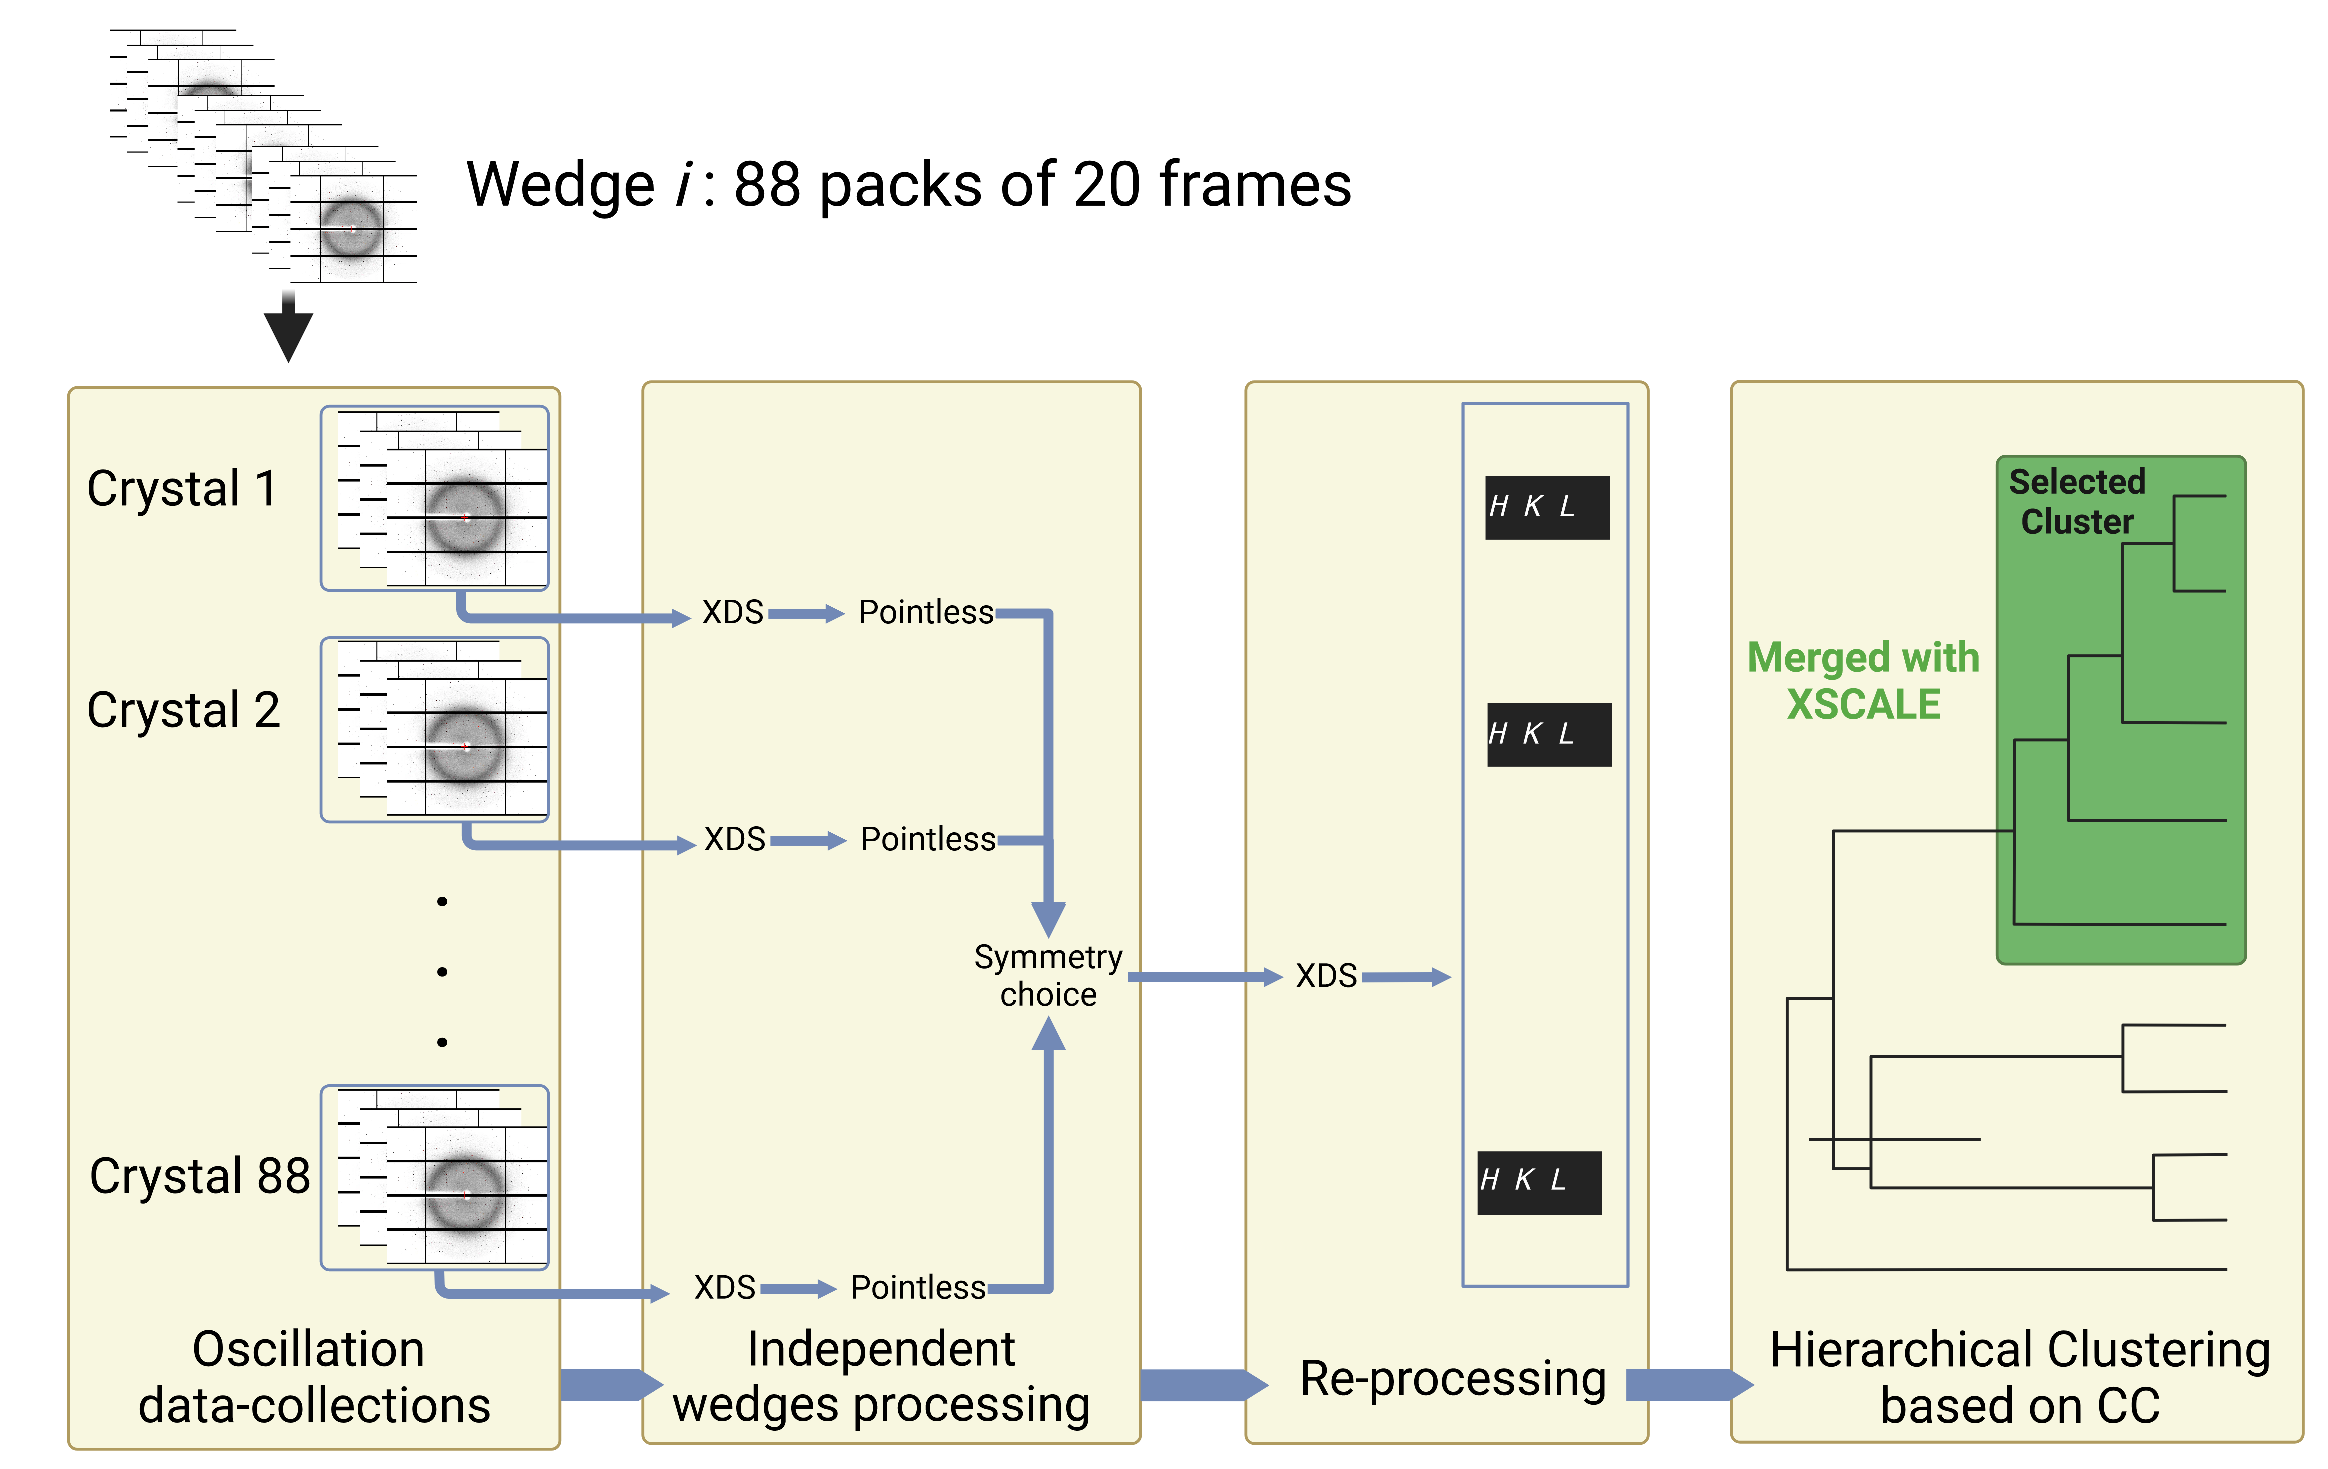
\includegraphics[width=\textwidth]{images/cracry/TR-SOX_data-analysis.pdf}
  \hfill
  \caption{Data processing scheme: All wedges with the same timestamp are processed jointly. First, the individual wedges are indexed with XDS \parencite{kabschXDS2010}, and their symmetry is determined by Pointless \parencite{evansIntroductionDataReduction2011}. Then, the most abundant symmetry is chosen, and an average of all lattice parameters from wedges presenting this symmetry is calculated as the consensus set of lattice parameters. All wedges undergo a second round of indexing by XDS, using this majority symmetry and consensus lattice parameters as prior knowledge. All sets of structure factors produced this way are clustered using a distance metric based on the correlation coefficient of the intensities. The Cluster with the highest \(CC_{1/2}\) in its outer shell while maintaining an I/\textsigma(I) of 1.5, as well as an overall completeness of 93 \%, is automatically chosen.  This data processing scheme is based on Kamo \parencite{yamashitaKAMOAutomatedData2018}, with added automation of particular steps.}\label{fig:TR-SOX_proc}
\end{figure}

\subsection{Observing the unravelling of \textalpha22 with TR-MX, at last}

Throughout the data collection, the C-axis maintains its length from 0 to 2.5 s and then shrinks from 154.0 \AA\ initially to 150.5 \AA\ (red diamonds in Fig. \ref{fig:TR-SOX_qFo} (f)), close to the lattice parameters of steady-light. This suggests that the steady illuminated-state might be achieved by the 5.8 s mark. However, this lack of isomorphism prevents us from analysing the last datasets in the series via isomorphous difference \(F_{obs}(wedge_i) - F_{obs}(dark\mbox{-}SOX)\) electron density map. Unfortunately, the real-space difference map approach used for steady-light and dark structures (Fig. \ref{fig:TR-SOX_ligh_dark_steady_CraCRY} (a)) did not produce meaningful results for these 'late' (> 3 s) datasets. This is likely a consequence of the lower data quality of these last datasets compared to the steady-illuminated and dark structures discussed previously. Indeed, as X-ray dose piles up on the crystals (797 kGy for the full rotation, meaning 26 additional kGy per wedge, calculated with RADDOSE 3D, \cite{buryEstimateYourDose2018}), diffraction resolution of the datasets decreases sharply because of global radiation damage (blue dots in Fig. \ref{fig:TR-SOX_qFo} (f)). 


Therefore, at first, only wedges recorded from 200 ms to 2.8 s after the start of the illumination were analysed. The isomorphous maps were Q-weighted \parencite{ursbyImprovedEstimationStructureFactor1997} using XtraPol8 \parencite{dezitterXtrapol8EnablesAutomatic2022} for representation purposes, as they are more readable than the non-weighted experimental maps when observed over the entire protein. Crucially, the experimental and weighted maps present the same features; only the signal/noise ration is affected by the weighting. 

200 ms after the beginning of the illumination, the Q-weighted difference map features the same pair of peaks around D321 (coloured green in Fig. \ref{fig:TR-SOX_qFo} (a)) as that visible in the 200 ms pump-probe TR-SFX time point (Fig. \ref{fig:CraCRY_Cter} (d)). A pair of peaks around N395 (Fig. \ref{supfig:TR-SOX_qFo_FAD} (a)) indicates that the O\textdelta1 atom of its carboxamide head has moved closer to the N5 atom of the isoalloxazine ring of the flavin, in the same fashion to the 200 ms pump-probe TR-SFX time point (Fig. \ref{fig:CraCRY_protonation} (c)), albeit with a greatly weaker signal.  A negative electron density peak on R492 (coloured purple in Fig. \ref{supfig:TR-SOX_qFo_FAD} (a)) indicates that the D321/R492 interaction has indeed been ruptured. This map resembles a lower-resolution version of the 200 ms pump-probe time-point, validating the overlap between the TR-SFX and TR-SOX series. 

400 ms after the beginning of the illumination, and in every later time point, more negative difference electron density builds up on \textalpha22, indicating that the helix gradually becomes disordered. However, the signal around N395 disappears past 200 ms (Fig. \ref{supfig:TR-SOX_qFo_FAD} (b), (c), (d) and (e)) while the pair of peaks on D321 weakens until 600 ms and has completely disappeared at the 800 ms mark. Whether these precise features disappear because of the disordering of the strand carrying D321, and decay of the transient stabilisation of the FADH\textsuperscript{•}, or whether they are lost because of a loss of signal due to the global decay in resolution of the datasets over time (Fig. \ref{fig:TR-SOX_qFo} (f)) is difficult to ascertain. 

\begin{figure}[H]
  \centering
  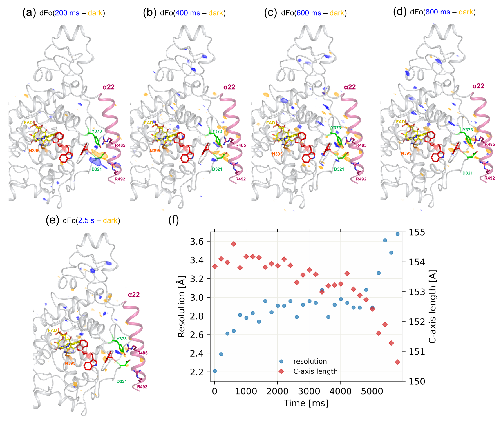
\includegraphics[width=\textwidth]{images/cracry/TR-SOX_qFo.pdf}
  \hfill
  \caption{TR-SOX data up to 3 s. Overall view of Q weighted \parencite{bourgeoisNewProcessingTools1999, dezitterXtrapol8EnablesAutomatic2022} Isomorphous \(F_{obs}(time\ point) - F_{obs}(dark)\) maps from the TR-SOX experiment, contoured at 3.0 \textsigma level (the \textsigma level had to be lowered from 3.5 to 3.0 to represent the maps because their resolution is much lower than those produced by the TR-SFX experiment). (a) In 200-SOX, (b) 400-SOX, (c) 600-SOX, (d) 800-SOX, (e) 2500-SOX.  In 200-SOX, a pair of peaks on D321 indicates that its side chain has flipped. Light negative density on \textalpha22 indicated that it is starting to become flexible. In 400-SOX and until 800-SOX, the signal on D321 dwindles, while the strength of the negative electron density on \textalpha22 builds up. In 2500-SOX, overall signal levels have decreased significantly. Negative peaks on \textalpha22 and the strands involved in its stabilisation are still visible. (f) Decrease of resolution and shrinking of the unit cell over time. Resolution initially decreases extremely fast from 2.2 to 2.8 \AA\ over the first second, then plateaus until 5 s, at which point it drops drastically again. The value of the C-axis lattice parameter stays stable until \textasciitilde3.0 s, at which point the C-axis start shrinking extremely fast.}\label{fig:TR-SOX_qFo}
\end{figure}

\subsection{SVD deconvolution of a TR-SOX series}\label{sec:TR-SOX_SVD}

SVD analysis of the TR-SOX series from 200 ms to 2.8 s yields two meaningful components. The signal in the first time-invariant structural component lSV0 is concentrated in the region surrounding \textalpha22 (Fig. \ref{fig:TR-SOX_SVD} (a)), similarly to the \(steady\mbox{-}state - dark\) real space difference map (Fig. \ref{fig:TR-SOX_ligh_dark_steady_CraCRY} (a)). Negative difference electron density covers the entirety of  the backbone of \textalpha22 (coloured purple) as well as the strands carrying D321 (coloured green). Pairs of peaks around Y373 reveal that it is adopting the same conformation as the one it occupies in steady-light (blue in Fig. \ref{fig:TR-SOX_ligh_dark_steady_CraCRY} (b)). 

There are, however, two substantial differences between lSV0 and the \(steady\mbox{-}state - dark\) real space difference map. \textbf{(1)} The absence of negative difference electron density on the N314: C317 (bottom half of CraCRY in Fig. \ref{fig:TR-SOX_ligh_dark_steady_CraCRY} (a)) in lSV0, hints that the disordering of the PHr domain is not fully achieved in the intermediate represented by lSV0. \textbf{(2)} The positive electron peaks on the loop positioned over \textalpha22 (P442: P453) and the helix over the flavin cofactor (T337: W352) visible in lSV0 (Fig. \ref{fig:TR-SOX_SVD} (a)), which are not present in the \(steady\mbox{-}state - dark\) real space difference map. That second point suggests that the intermediate represented by lSV0 corresponds to a state of CraCRY in which the loops between the flavin cofactor and the hinge region of the helix are transiently adjusting to the newly disordered \textalpha22, and the N-terminal part of the strand carrying D321 has not fully disordered yet.

The signal in the second time-invariant structural component lSV1 (Fig. \ref{fig:TR-SOX_SVD} (b)) is focused on D321 and N395. Its main feature is the pair of peaks pattern indicating the flip of the D321 side chain (close-up view in Fig. \ref{fig:TR-SOX_SVD} (d)), and its second feature is the shift of the O\textdelta1 atom of N395 towards the N5 atom of the flavin chromophore (Fig. \ref{fig:TR-SOX_SVD} (c)). 

The amplitude of rSV0 (coloured black) grows in two steps over the TR-SOX series, a first seemingly logarithmic growth from 0 to 1.2 s, and then a second more linear growth phase from 1.6 s to the end of the series (Fig. \ref{fig:TR-SOX_SVD} (e)). While the amplitude of the second component rSV1 (red) is initially barely stronger than rSV0, it plateaus around 10 until 1.4 s, meaning it starts to be overtaken by rSV0. In a second phase, it decreases until its polarity is inverted from 1.6 s to 2.8 s. With that in mind, it is clear that lSV1 is a modulating factor of lSV0 (similar to the case of the SwissFEL ps-ns series of DNA repair in \textit{Mm}CPDII presented in Fig. \ref{fig:SwissFEL_SVD_MmCPDII}). The combination of equally weighted lSV0 and lSV1 at 200 ms produces the state observed at the end of the TR-SFX series (Fig. \ref{fig:CraCRY_Cter} (d) and Fig. \ref{fig:CraCRY_protonation} (c)). 

The SVD analysis demonstrates that the flip of D321 and the transient stabilisation of the FADH\textsuperscript{•} do not disappear quickly after 200 ms as a simple observation of the Q-weighted isomorphous difference \(F_{obs}(wedge_i) - F_{obs}(dark\ wedge)\) suggested (Fig. \ref{fig:TR-SOX_qFo}). Rather, the signal corresponding to these features (represented by the trend of rSV1 over time in Fig. \ref{fig:TR-SOX_SVD} (c)) remains, but is increasingly dominated by the signal corresponding to the increasing disorder of \textalpha 22, and the nearby strands of the PHr domain. Instead, the signal from the flip of D321 seems to disappear from the 1.5 s mark. 

\begin{figure}[H]
  \centering
  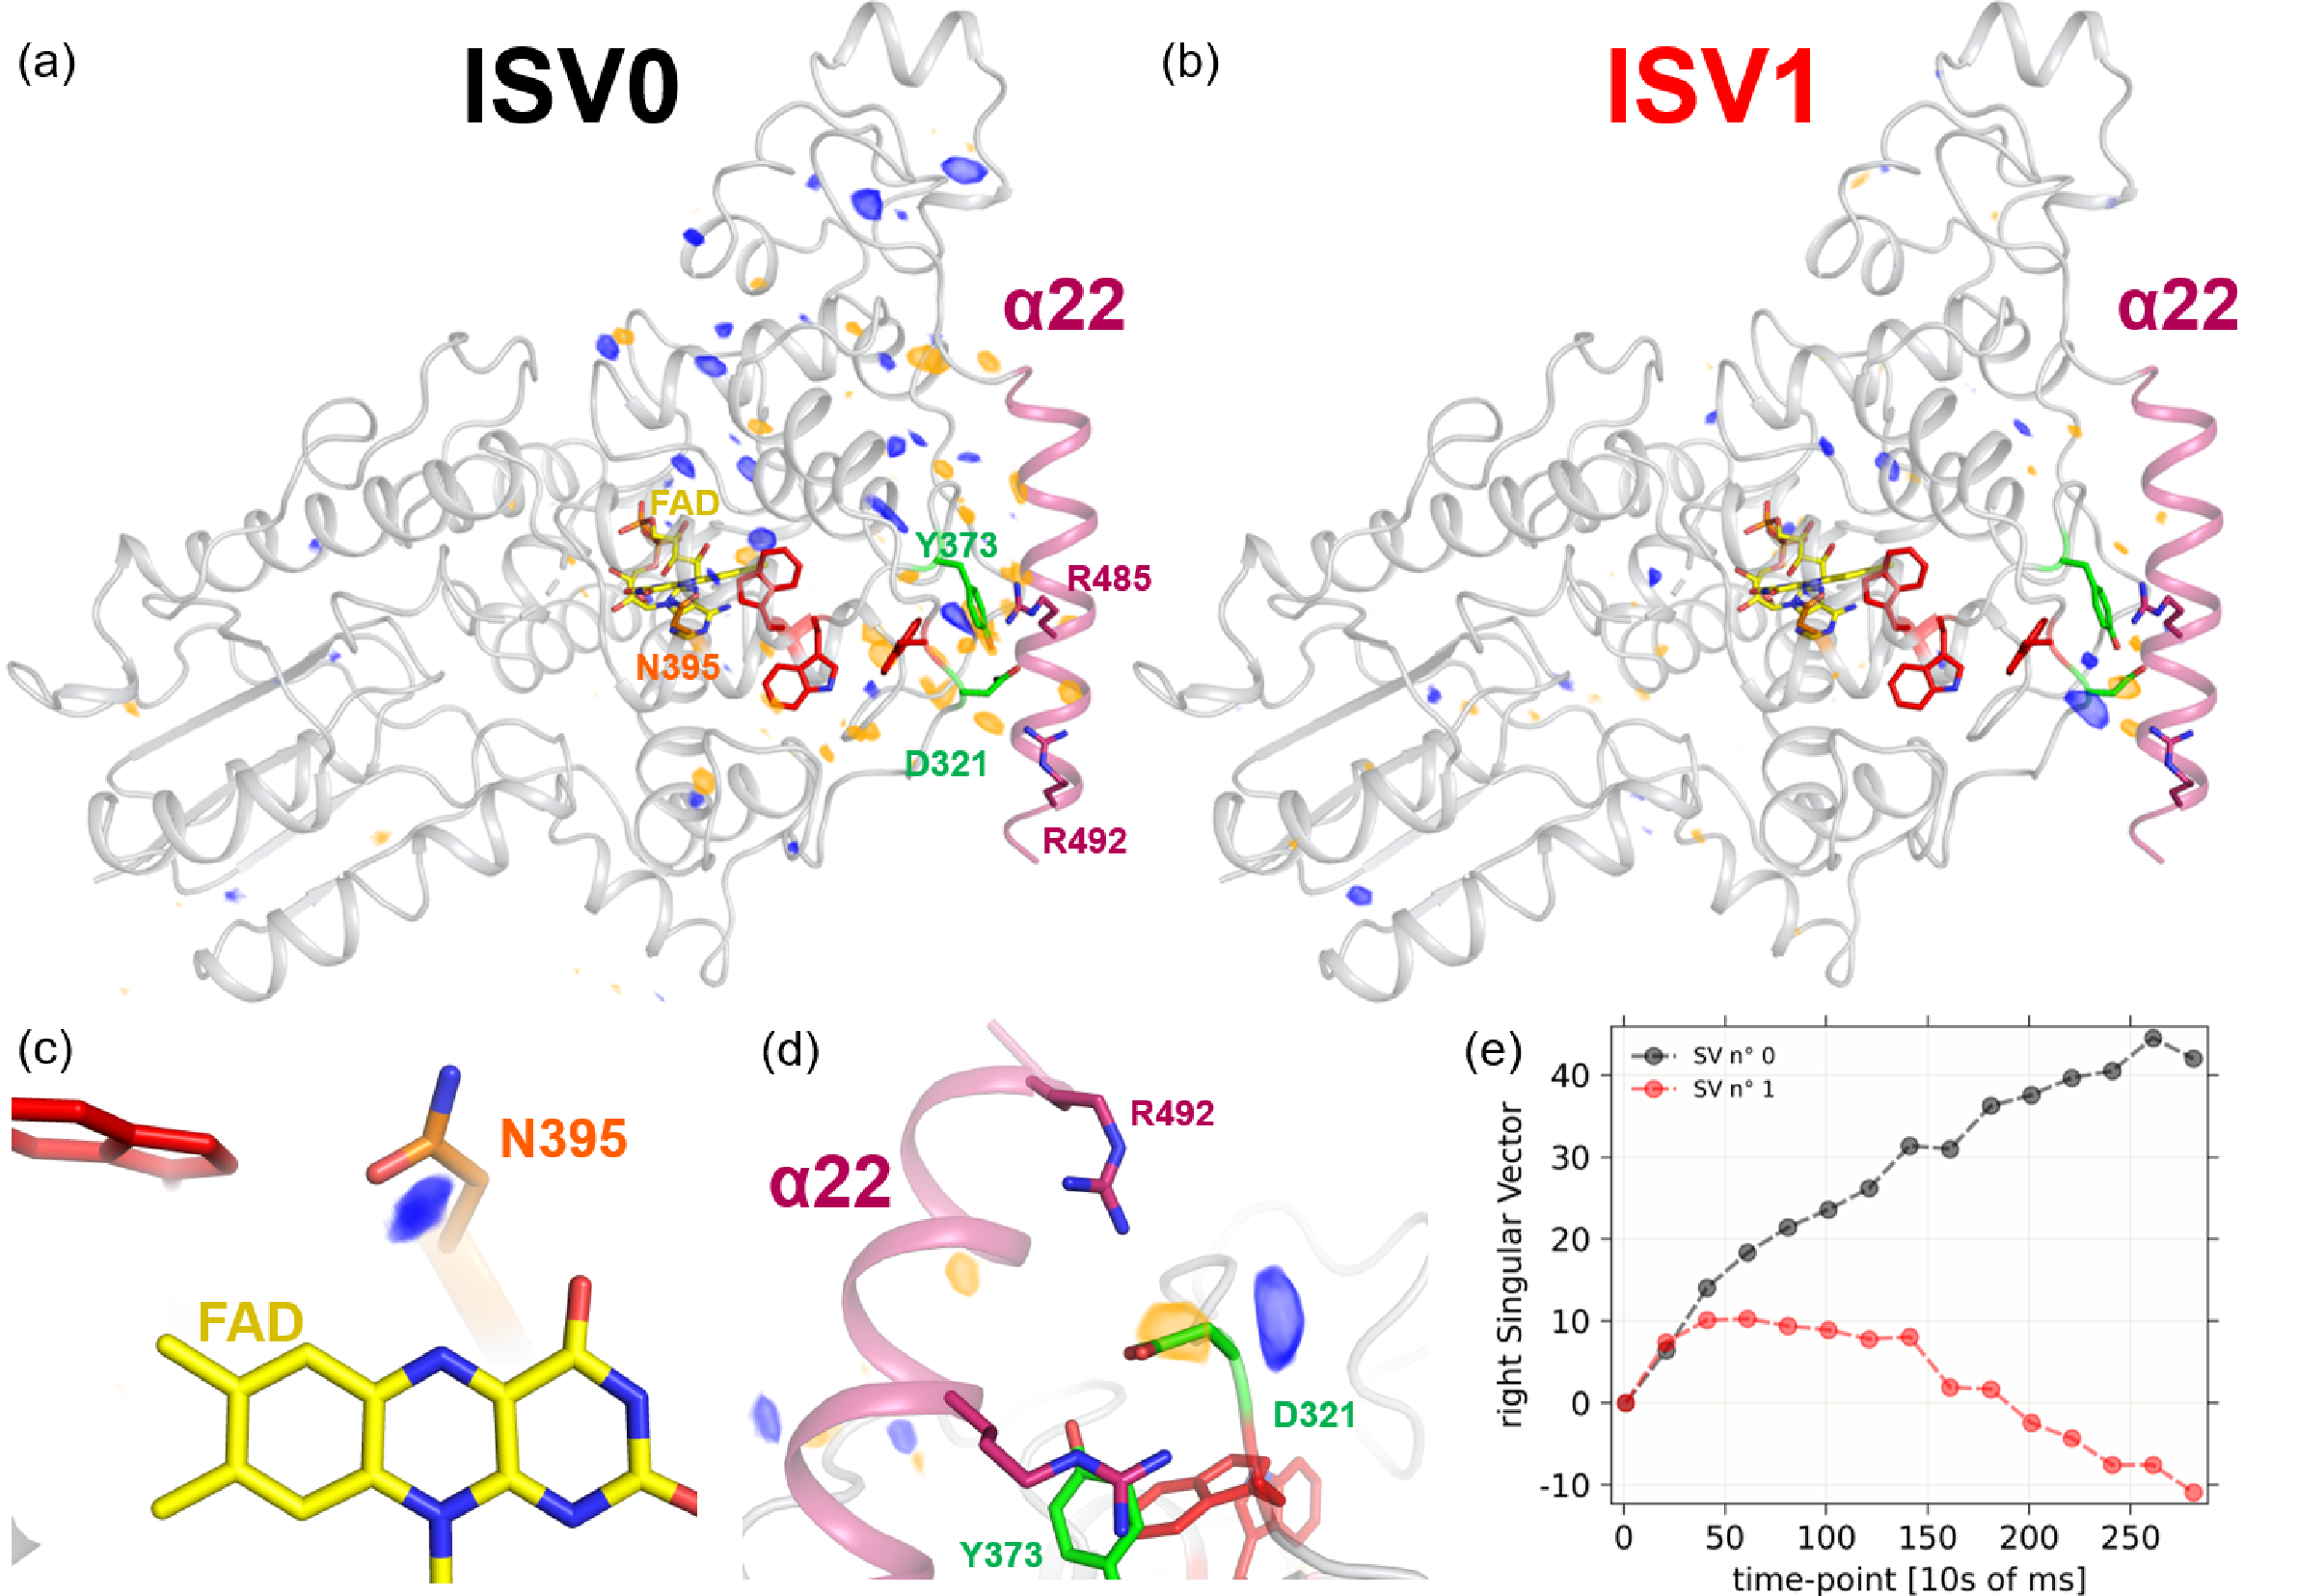
\includegraphics[width=\textwidth]{images/cracry/TR-SOX_SVD.pdf}
  \hfill
  \caption{SVD analysis illustrates the transition from local perturbation of the D321/Y492 interaction to the unravelling of \textalpha22 and supporting PHr strands. lSVx the signal is contoured at 3.0 \textsigma level (positive peaks in blue, negative peaks in gold). (a) The main time-invariant structural component (lSV0) features negative difference electron density all along \textalpha22, as well as the strands involved in the interaction with \textalpha22. A pair of positive and negative peaks around Y373 indicate that it shifts to a new position to occupy the space vacated by R485. (b) The signal contained in lSV1 is focused, compared to that of lSV0: it contains the pair of peaks of the flipped D321, and the positive peak between N395 and the FAD, reminiscent of the post-protonation stabilisation of the FAD radical observed in Chapter \ref{chap:CraCRY_TR-SFX_1}. (c) FAD-centred view of the N395 feature contained in lVS1. (d) Close-up view of the D321 flip feature present in lSV1. (e) Evolution of the time-dependent rSVs over the first half of the series (0-2.8 s). rSV0 (black) is initially weaker than rSV1, and overtakes it by 400 ms, before building up steadily over the series. rSV1 (red) is the main component of the first time point of the series (200 ms), then plateaus until 1.4 s. From 1.4 s to 2.5 s, it decays very quickly and switches polarity.}\label{fig:TR-SOX_SVD}
\end{figure}

\subsection{A domino mechanism from the rupture of D321/R494 to the disordering of \textalpha22 and its support strands}

The difference in kinetics between the large-scale disordering of \textalpha22 and its support strands (beige-coloured segments in Fig. \ref{fig:TR-SOX_ligh_dark_steady_CraCRY} (b)) represented by the trend of rSV0, and the disruption of the strand carrying D321 and W322 suggests a disordering mechanism consisting in at least three elements, with each causing the next in the same fashion as a domino falls over the next. The first of these elements is the disordering of the D321/R492 interaction, represented by the features of lSV1 (Fig. \ref{fig:TR-SOX_SVD} (b)), which causes the disorder of the tip of the \textalpha22 helix, as visible in the local SVD analysis of the TR-SFX series (lSV0, represented in \ref{fig:CraCRY_Cter-SVD} (a)). 

Once the tip of \textalpha22 becomes disordered, the strand carrying D321 is exposed to the solvent and unfolds quickly (relative to the time-scale of the TR-SOX experiment) at the 1.6 s mark. This is evidenced by the brutal decay of rSV1 at the 1.6 s mark; the loss of the pair of peaks around D321 indicates that it has become disordered. This is the second element of the mechanism. 

As a consequence of the unfolding of the strand carrying D321, the mid-section of \textalpha22 is exposed to the solvent, and quickly dissociates from the PHr domain, allowing Y373 to twist, as evidenced by the existence of the second growth phase of rSV0 (Fig. \ref{fig:TR-SOX_SVD} (e)). This rapid dissociation causes transient rearrangements in the loop over and the helix under the hinge connecting \textalpha22 to the rest of the PHr domain. This is the third element of the mechanism and is represented by the features of lSV0 (Fig. \ref{fig:TR-SOX_SVD} (a)). 

The putative signalling state identified in steady-light structure (coloured blue in \ref{fig:TR-SOX_ligh_dark_steady_CraCRY} (b)) is not achieved at the 2.8 s mark when the SVD analysis ends. At some point after 2.8 seconds, the N-terminal end of the loop carrying D321 (N314: C317) becomes disordered, while the transient rearrangements around the hinge of \textalpha22 begin to stabilize. This is quite probably linked to the shrinkage of the C-axis observed from 4 s to 5.8 s. An analysis of the remaining wedges using methods that do not rely on isomorphism and are tolerant to low resolution is currently underway in collaboration with Yuhei Hosokawa, from Manuel Maestre-Reyna's group at the NTU. At the time of writing this manuscript, it has not fully converged yet. 

\section{Conclusion}

Despite its lower resolution, the TR-SOX series perfectly complements the high-resolution data collected in the ns-ms time scale at SACLA. This could only be achieved through the use of the SVD analysis, which is especially suited to the analysis of TR-SOX data. The combined TR-SFX and TR-SOX series draft a sequence of events from the last step of the electron transfer chain, the proton-coupled electron transfer between D321 and Y373 (corresponding to the state represented in \ref{fig:CraCRY_Cter} (a)), and the rise of a signalling state (blue model in Fig. \ref{fig:TR-SOX_ligh_dark_steady_CraCRY} (b)) which is consistent with the results of a recent study of CraCRY in solutions \parencite{zanglTimeResolvedIonMobility2024}. In combination with the recent study of the closely related 6-4 photolyase from \textit{Drosophila melanogaster} by TR-SFX \parencite{celliniDirectedUltrafastConformational2024}, our TR-SFX and TR-SOX results map the entire photoreaction of CraCRY as a photoreceptor. 